% \newcommand{\prototitle}{Versuch 2 - Statistik}
% \newcommand{\Fachbereich}{Praktikum Messtechnik}
% \input{../packages/tu_header}

\newcommand{\institut}{Institut f\"ur Telekommunikationssysteme}
\newcommand{\fachgebiet}{Nachrichten\"ubertragung}
\newcommand{\veranstaltung}{Praktikum Nachrichten\"ubertragung}
\newcommand{\pdfautor}{\"Ozg\"u Dogan (326 048), Boris Henckell (325 779)}
\newcommand{\autor}{\"Ozg\"u Dogan (326 048)\\ Boris Henckell (325 779)}
\newcommand{\gruppe}{Gruppe: }
%\newcommand{\betreuer}{Betreuer: Mahmoud Felk}


\newcommand{\pdftitle}{Nachrichten\"ubertragung\ Praktikum\ 03}
\newcommand{\prototitle}{Praktikum 01 \\ Einf\"uhrung in MATLAB}


\input{../../packages/tu_header_8}


% \lstlistoflistings
\definecolor{darkgray}{rgb}{0.95,0.95,0.95}
\definecolor{darkolivegreen}{HTML}{01a801}
\definecolor{functionsBlue}{HTML}{32b9b9}
\definecolor{variableRed}{rgb}{1,0,0}
\definecolor{stringBrown}{HTML}{bc8e8e} % f geht nicht

\lstset{
        %\lstset{extendedchars=true} % Umlaute an der richtigen stelle und nicht am Anfang ausgeben
        %basicstyle=\footnotesize\ttfamily,
        basicstyle=\small,
        %
        inputencoding=utf8,
        %
        tabsize=4,
        showspaces=false,
        showtabs=false,
        showstringspaces=true, % no special string spaces
        %
        backgroundcolor=\color{darkgray}, % background
        stringstyle=\color{stringBrown}\fseries, % Strings
        keywordstyle=\color{functionsBlue}\bfseries, % keywords Blau
        identifierstyle=\color{variableRed}, % variablen
        commentstyle=\color{darkolivegreen}, %  comments
        %
        breaklines=true,
        %
        numbers=left,
        numberstyle=\tiny,
        stepnumber=1,
        numbersep=7pt,
        %
        frame=single,
        columns=flexible,
        %
        xleftmargin=-2cm,
        xrightmargin=-1.5cm,
        %
        language=Matlab
}

%---------------------------------------------------------------------
%---------------------------------------------------------------------
%---------------------------------------------------------------------

\section{Einleitung}
\begin{quote}
	In diesem Termin wurde durch praktisches Aufbauen und Testen von modulierenden
	Übertragungsstrecken das Prinzip der Amplitudenmodulation (AM) und der
	Frequenzmodulation (FM) nachvollzogen. Dafür wurde zuerst immer das nötige
	Signal erzeugt, welches dann moduliert und auch demoduliert wurde.
\end{quote}
%--------------------------------------------------------------------
%--------------------------------------------------------------------    
\section{Theorie Modulation}
\begin{quote}
        Um Signale an spezielle Kanaleigenschaften anzupassen lassen sich diese Signale durch eine Modulation in
        Amplitude und Frequenz verändern.\\
        Dies hat beispielsweise den Vorteil, dass sich die Signale anschließend mit einer Frequenz
        übertragen lassen auf der die Rauscheinflüsse geringer sind. Des weiteren entsteht durch Modulation die
        Möglichkeit mittels Multiplexing mehrere Signale gleichzeitig über einen Kanal zu übertragen und diese im
        nachhinein eindeutig unterscheinden zu können.\\
        Um das Ursprungssignal auf der Empfängerseite nutzen zu können muss es realisierbare Demodulationsmethoden
        geben.
\end{quote}


\section{Amplitudenmodulation}
\begin{quote}
	\subsection{Theorie}
    \begin{quote}
        Bei der Amplituden Modulation wird aus dem Nutzsignal$u(t)$ mit einer variablen Amplitude und Frequenz ein
        Moduliertes Signal mit einer festen Frequenz und variabler Amplitude. Dazu wird $u(t)$ mit einem
        höherfrequenten Trägersignal $c(t)$ multipliziert. Daraus resultiert ein Signal mit der Frequenz des
        Trägersignals und einer Amplitude, die von dem Nutzsignal gesteuert wird.
        
        \begin{equation*}
        	\begin{split}
        		u_m(t) = A_c [u(t)] \cdot cos(\omega_c t)
        	\end{split}
        \end{equation*}
        
        Es gibt zwei verschiedene Möglichkeiten dieser Modulation. Erstens die Amplituden Modulation ohne Träger und die
        Amplituden Modulation mit Träger.
        
        \subsubsection{Amplitudenmodulation ohne Träger}
		\begin{quote}
			Bei dieser Art der Amplitudenmodulation wird die Amplitude linear durch das Nutzsignal gesteuert. Das bedeutet für
			die Amplitude des modulierten Signals:
			
			\begin{equation*}
            	\begin{split}
            		A_c [u(t)] = k \cdot u(t)
            	\end{split}
            \end{equation*}
            
            
            Welche Auswirkung diese Art der Modulation auf ein Signal hat zeigt das folgende Bild sehr anschaulich. 
            
            \begin{figure}[H]
            \centering
                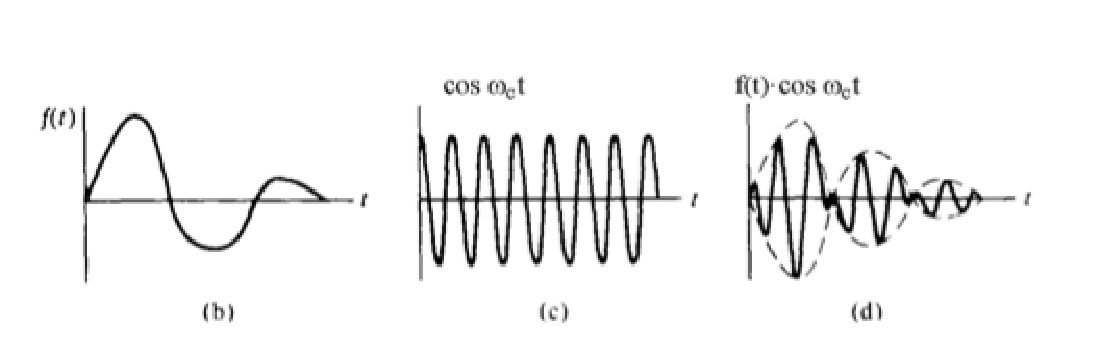
\includegraphics[scale=0.7, trim = 0cm 0cm 0cm 0cm, clip]{./Bilder/AMohneTraeger}
                    \caption{Amplitudenmodulation ohne träger}
                    \label{fig:AMohneTraeger}
                    \cite{AMohnetraeger}
            \end{figure}
    
            Um dieses modulierte Signal am Empfänger wieder zu demodulieren wird es noch ein weiteres mal mit dem
            Trägersignal multipliziert und anschließend Tiefpassgefiltert. Welche Auswirkung das hat zeigt folgendes
            Bild.
            
            \begin{figure}[H]
            \centering
                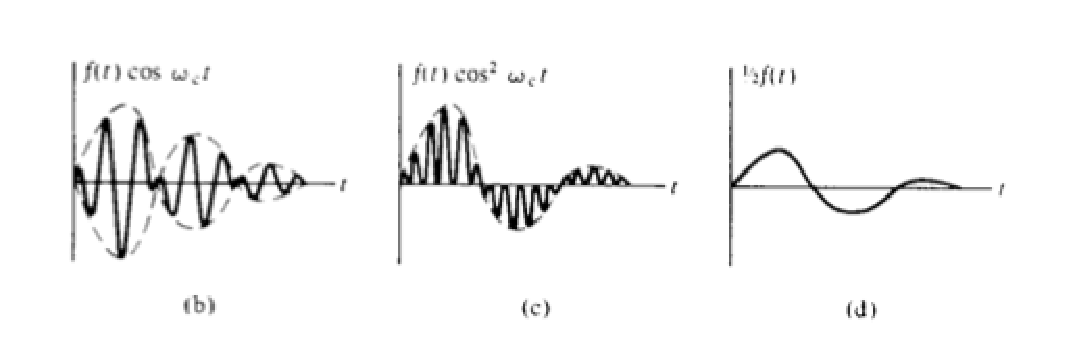
\includegraphics[scale=0.7, trim = 0cm 0cm 0cm 0cm, clip]{./Bilder/AMohnetraegerdemodulation}
                    \caption{Amplitudendemodulation ohne Träger}
                    \cite{AMdemodulation}
            \end{figure}
    
            Die Gesamte Übertragungsstecke der Amplitudenmodulation ohne Träger ist hier zu sehen.
            
            \begin{figure}[H]
            \centering
                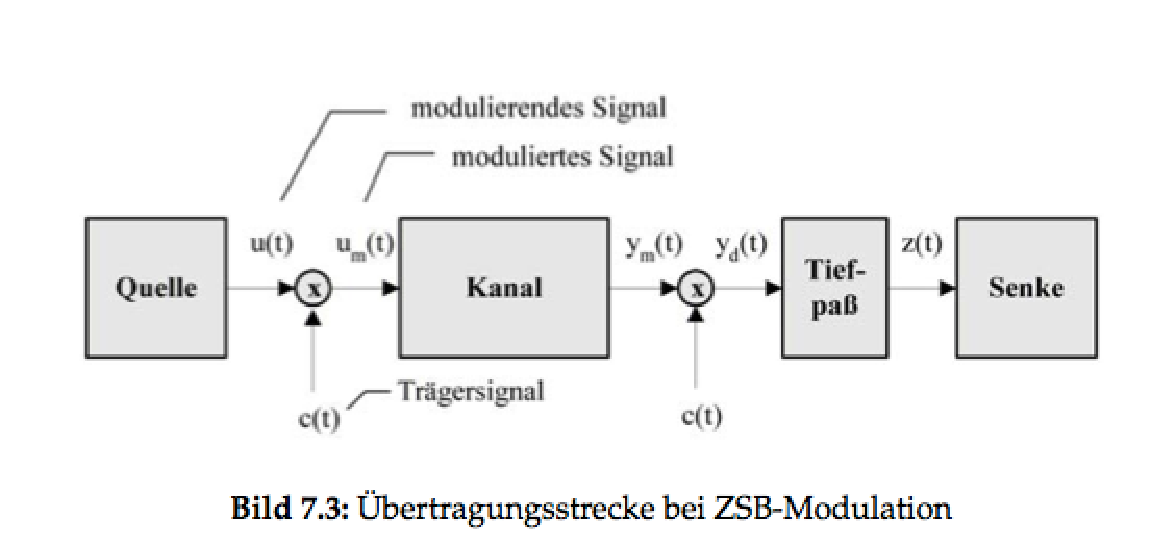
\includegraphics[scale=0.7, trim = 0cm 0cm 0cm 0cm, clip]{./Bilder/uebertragungsstreckeAMohnetraeger}
                    \caption{Übertragungsstrecke AM ohne Träger}
                    \cite{AMohneUeber}
            \end{figure}
             
             Damit diese Modulation jedoch Fehlerfrei funktioniert wird am Empfänger das kohärente Trägersignal
             benötigt. Das Bedeutet, dass das Trägersignal in exakt der selben Phase und Frequenz am Empfänger vorhanden
             sein muss. Ist das nicht der Fall kommt es zur Verfälschung des Nutzsignals bei der Demodulation.\\
             Da das jedoch schwer zu realisieren ist wurde die zweite art der Amplitudenmodulation entwickelt:
             Amplitudenmodulation mit Träger.
             
            
		\end{quote}
		
		\subsubsection{Amplitudenmodulation mit Träger}
		\begin{quote}
			Bei der Amplitudenmodulation mit Träger wird das Nutzsignal $u(t)$ bevor es mit dem Trägersignal $c(t)$
			multipliziert wird mit einem Offset versehen.
			
			\begin{figure}[H]
            \centering
                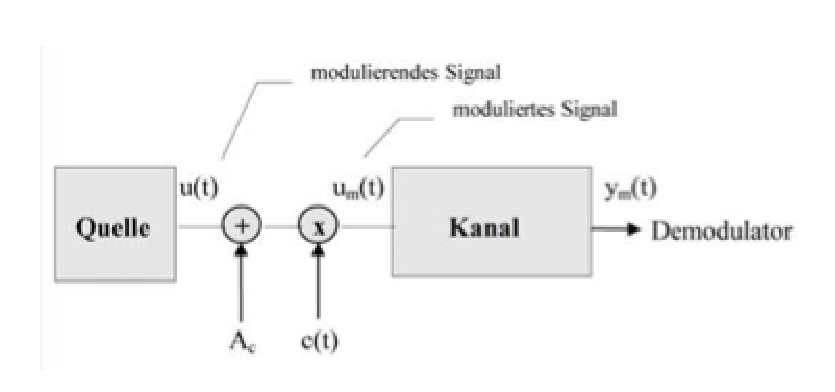
\includegraphics[scale=0.7, trim = 0cm 0cm 0cm 0cm, clip]{./Bilder/AMmitTraeger}
                    \caption{Amplituden Modulation mit Träger}
                    \cite{AMmitUeber}
            \end{figure}
            
            Das bedeutet für die Amplitude des modulierten Signals:
            
            \begin{equation*}
                \begin{split}
                    A_c [u(t)] = A + k \cdot u(t)
                \end{split}
            \end{equation*}
            
            Diese Art der Modulation hat folgende auswirkungen auf das Signal:
            
            \begin{figure}[H]
            \centering
                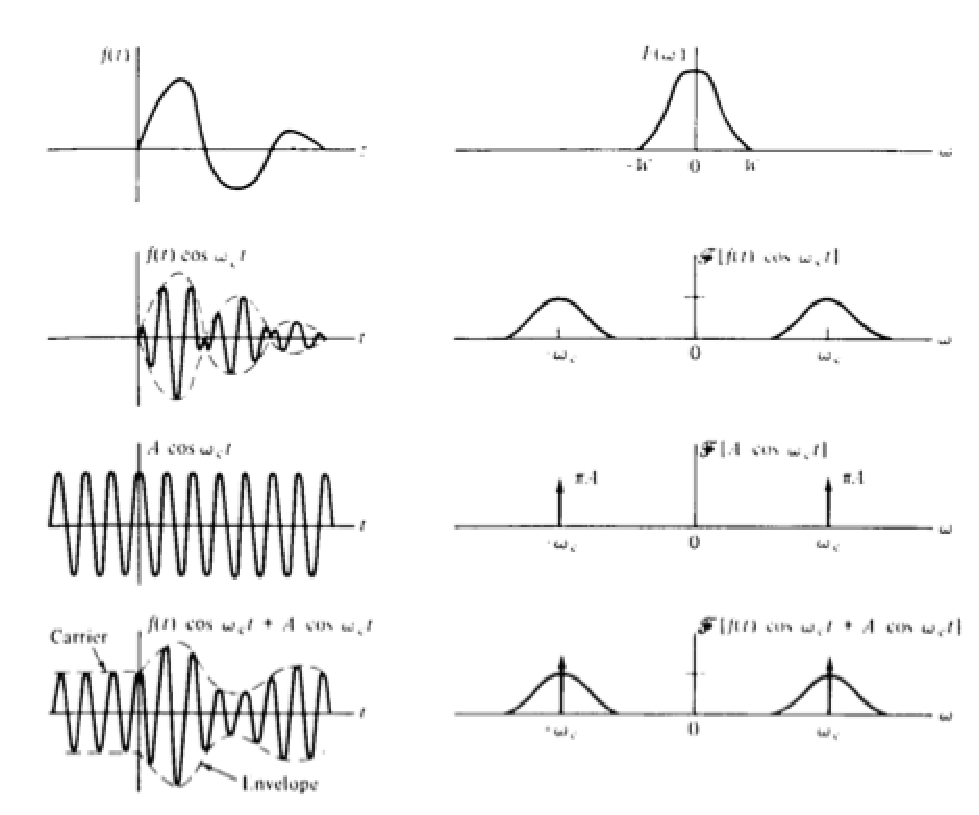
\includegraphics[scale=0.7, trim = 0cm 0cm 0cm 0cm, clip]{./Bilder/AMmittraegersignal}
                    \caption{Amplituden}
                    \cite{AMmitUeber}
            \end{figure}
            
            Für die Demodulation stehen bei diesem Verfahren zwei Möglichkeiten zur verfügung. Einerseits dieselbe
            Demodulation wie oben schon beschrieben, die erneute multiplikation mit dem Trägersignal.\\
            Andererseits lässt sich dieses Signal auch demodulieren indem das Signal gleichgerichtet wird und
            anschließend der Offset entfernt wird Außerdem muss auch dieses Signal Tiefpassgefiltert werden. Der Vorteil
            dieser zweiten Methode ist, dass sie sehr viel einfacher auf der Empfängerseite zu realisieren ist als die erst 
            Art der Demodulation.
    
		      
		\end{quote}
        
        
    \end{quote}
    
    \subsection{Vorbereitungsaufgabe}
    \begin{quote}
        Als Vorbereitung für die Messungen zum Thema Amplitudenmodulation haben wir mit Hilfe von Matlab verschiedene
        Signalformen simuliert und anschließend Amplituden moduliert.\\
        Dazu haben wir als Nutzsignal jeweils ein Rechtecksignal, ein Dreiecksignal sowie ein Cosinussignal mit
        einer Amplitude (von Nulldurchgang zum Spitzenwert) von $1V$ und einer Frequenz von $100 Hz$. Zusätzlich haben
        wir noch ein Trägersignal mit der selben Amplitude aber mit einer Trägerfrequenz von $2000 Hz$ erstellt.\\
        Anschließend haben wir die drei Nutzsignale Amplitudenmoduliert indem wir sie jeweils mit dem Tägersignal
        multipliziert haben.\\
        Zur Analyse haben abschließende diese modulierten Signale sowie ihre Amplituden- und Phasengänge platten
        lassen.\\
        In der Auswertung werden wir diese Ergebnisse anschließend mit den gemessenen Ergebnissen vergleichen.
    \end{quote}
    
    \subsection{Durchführung}
    \begin{quote}
    	\subsubsection{Signalerzeugung und Modulation}
    	\begin{quote}
    	Als Basisbandsignal generierten wir ein mittelwertfreier Sinus,
    	der eine Frequenz von $100 Hz$ und eine Amplitude von $1 V$ besaß. Dazu wurde noch
    	ein Offset von einem Volt addiert, welches wir mit dem Adder-Modul und der
    	Quelle Variable DCV verwirklicht haben. Somit hatte unser Basisbandsignal
    	keinen Nulldurchgang mehr. Mit den Verstärkerknöpfen g und G wurde die
    	Summe vom Sinus und Offset korrekt eingestellt und am Oszilloskop
    	korrigiert.\\
    	Nachdem unser Nutzsignal erstellt wurde, führten wir die Modulation anhand
    	einer Multiplikation mit dem Multiplier-Modul durch. Als Trägersignal
    	verwendeten wir dabei den $2kHz$-Sinus des Master-Signal-Moduls.\\
    	Nach der Untersuchung des Sinus-Basisbandsignals, wurde die Modulation auf
    	gleiche Weise noch mit dem Rechteck- und dem Dreiecksignal durchgeführt.
    	Die Ergebnisse aus dem Praktikum und der Vergleich mit den Ergebnissen aus
    	der Vorbereitungsaufgabe ist in der Auswertung zu finden.
    	\end{quote}
    	
    	\vspace{1em}
    	
    	\subsubsection{Synchrone Demodulation}
    	\begin{quote}
    	Nach der Amplitudenmodulation wurden die modulierten Signale auch
    	synchron demoduliert. Dies ermöglichten wir mithilfe des zweiten
    	Multiplier-Moduls und indem wir das Trägersignal erneut auf das modulierte
    	Signal multiplizierten. In einem Plot kann man sehen, dass das
    	Empfangssignal vierfache Amplitude besitzt als das Sendesignal.
    	Diese Abweichung korrigierten wir anhand eines Tiefpasses nach der
    	Demodulation.
    	
    	Ist das alles richtig so? was hatte Michael Tok denn gesagt? Auf jeden Fall
    	haben wir Messwerte zu demodulierten und demoduliert gefilterten Signalen.
    	Bei den gefilterten sind deutlich kleinere Amplituden zu sehen.
		\end{quote}    
    
    \end{quote}
    
    \subsection{Auswertung}
    \begin{quote}
        
        Hier kann man die Ergebnisse der Amplitudenmodulation sehen. Alle
        Nutzsignale hatten eine Frequenz von $100 Hz$, eine Amplitude von $1 V$
        und einen Offset von ebenfalls $1 V$. Das Trägersignal war ein $2
        kHz$-Sinus.
        
        In die minipages kommen immer die Vorbereitungsergebnisse und die
        Paktikumsergebnisse rein, damit sie miteinander verglichen werden
        können. Auf jeden Fall muss noch auf die Auswirkung der Veränderungen
        von Amplitude und Offset des Basisbandsignals eingegangen werden.
        
        
        \begin{center}
            \begin{tabular}{ll}

            \hspace{-10em}
                \begin{minipage}{0.6\textwidth}

                    \begin{figure}[H]
                        \label{fig:}
                        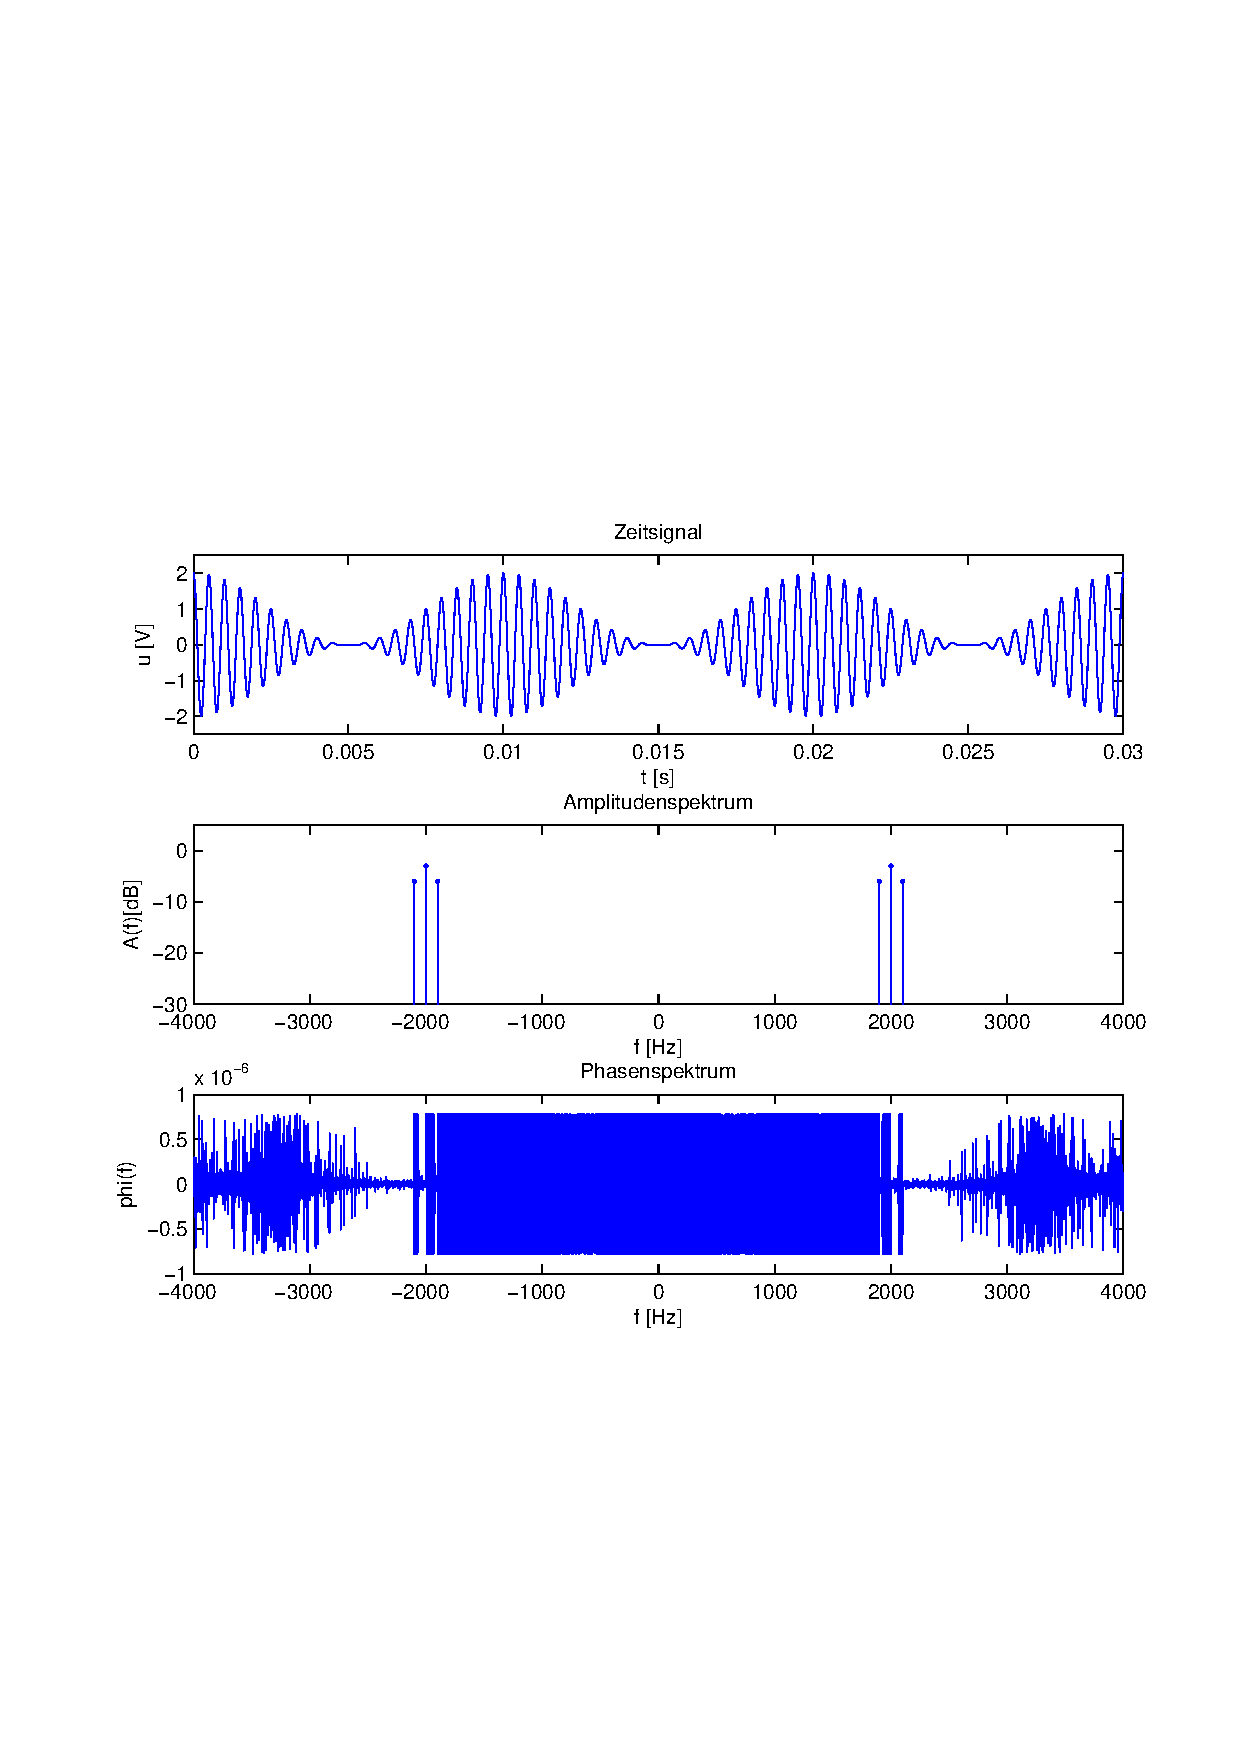
\includegraphics[scale=0.5, trim = 2cm 6.5cm 1.5cm
                        8.5cm, clip]{./Bilder/Cosinusmodsimuliert} %FIXME [width=640px,
                        % height=474px]
                        \caption{amplitudenmoduliertes Cosinussignal simuliert}
                    \end{figure}

                \end{minipage}
                \begin{minipage}{0.6\textwidth}

                     \begin{figure}[H]
                        \label{fig:}
                        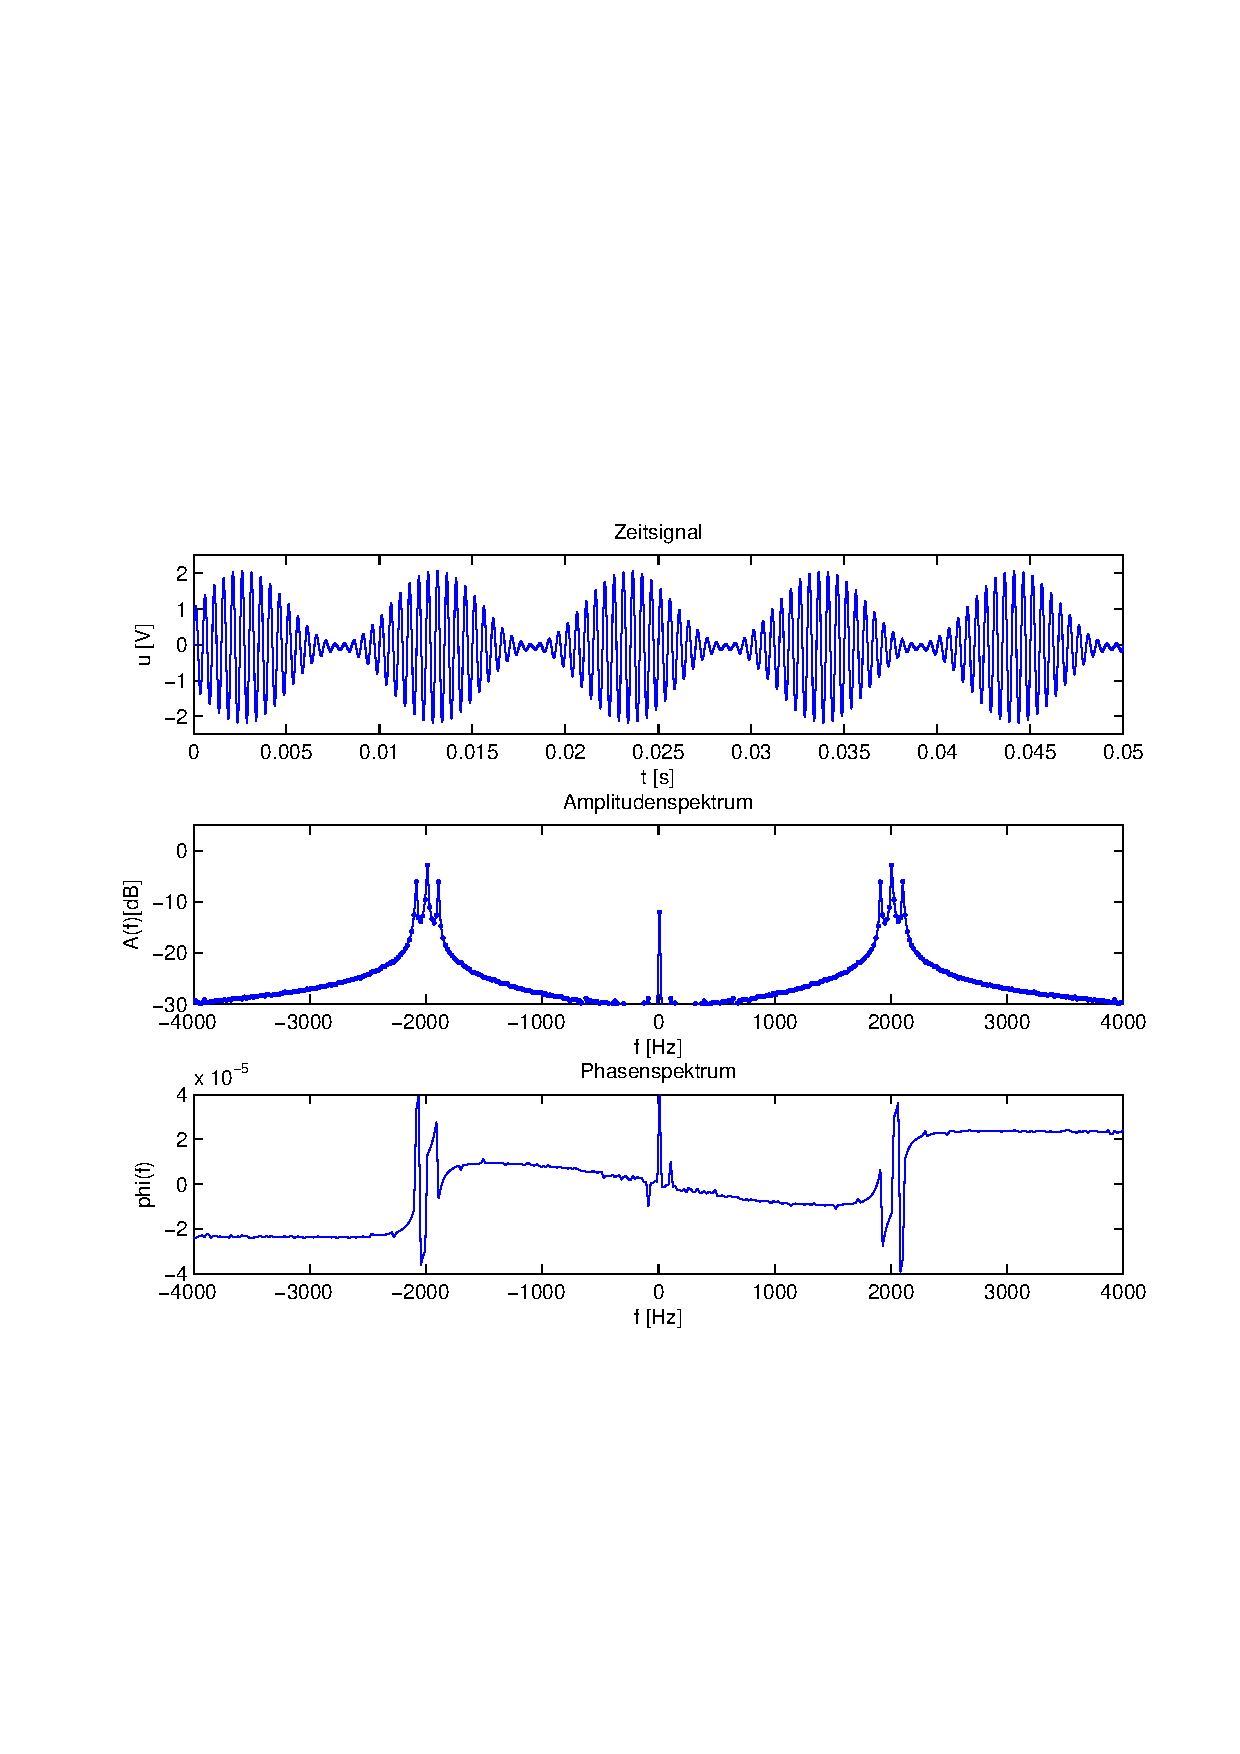
\includegraphics[scale=0.5, trim = 2cm 6.5cm 1.5cm
                        8.5cm, clip]{./Bilder/Cosinusmodgemessen} %FIXME
                        % [width=640px, height=474px]
                        \caption{amplitudenmoduliertes Cosinussignal gemessen}
                    \end{figure}
               \vspace{-1.5em}

                \end{minipage}

            \end{tabular}
            \end{center}
            
                    \begin{center}
            \begin{tabular}{ll}

            \hspace{-10em}
                \begin{minipage}{0.6\textwidth}

                    \begin{figure}[H]
                        \label{fig:}
                        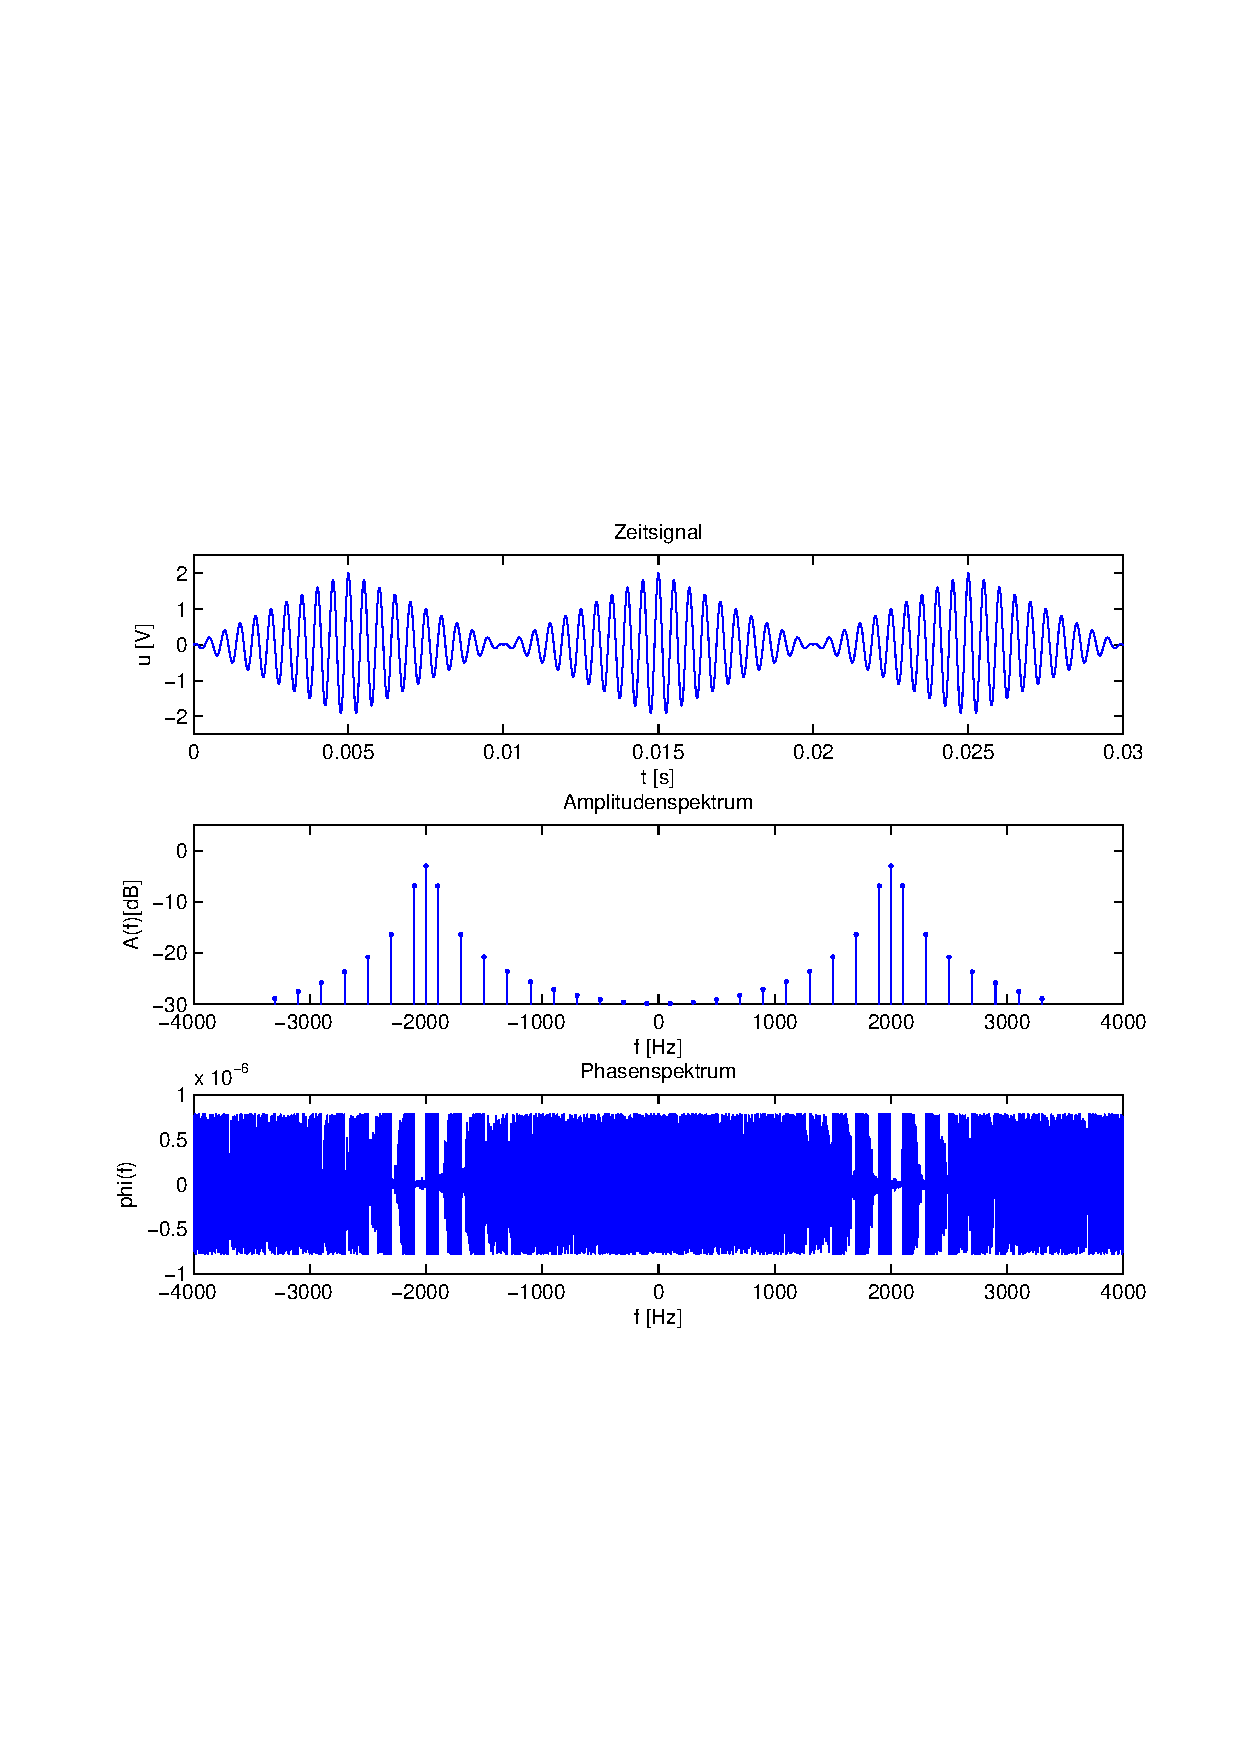
\includegraphics[scale=0.5, trim = 2cm 6.5cm 1.5cm
                        8.5cm, clip]{./Bilder/Dreieckmodsimuliert} %FIXME [width=640px,
                        % height=474px]
                        \caption{amplitudenmoduliertes Dreiecksignal simuliert}
                    \end{figure}

                \end{minipage}
                \begin{minipage}{0.6\textwidth}

                     \begin{figure}[H]
                        \label{fig:}
                        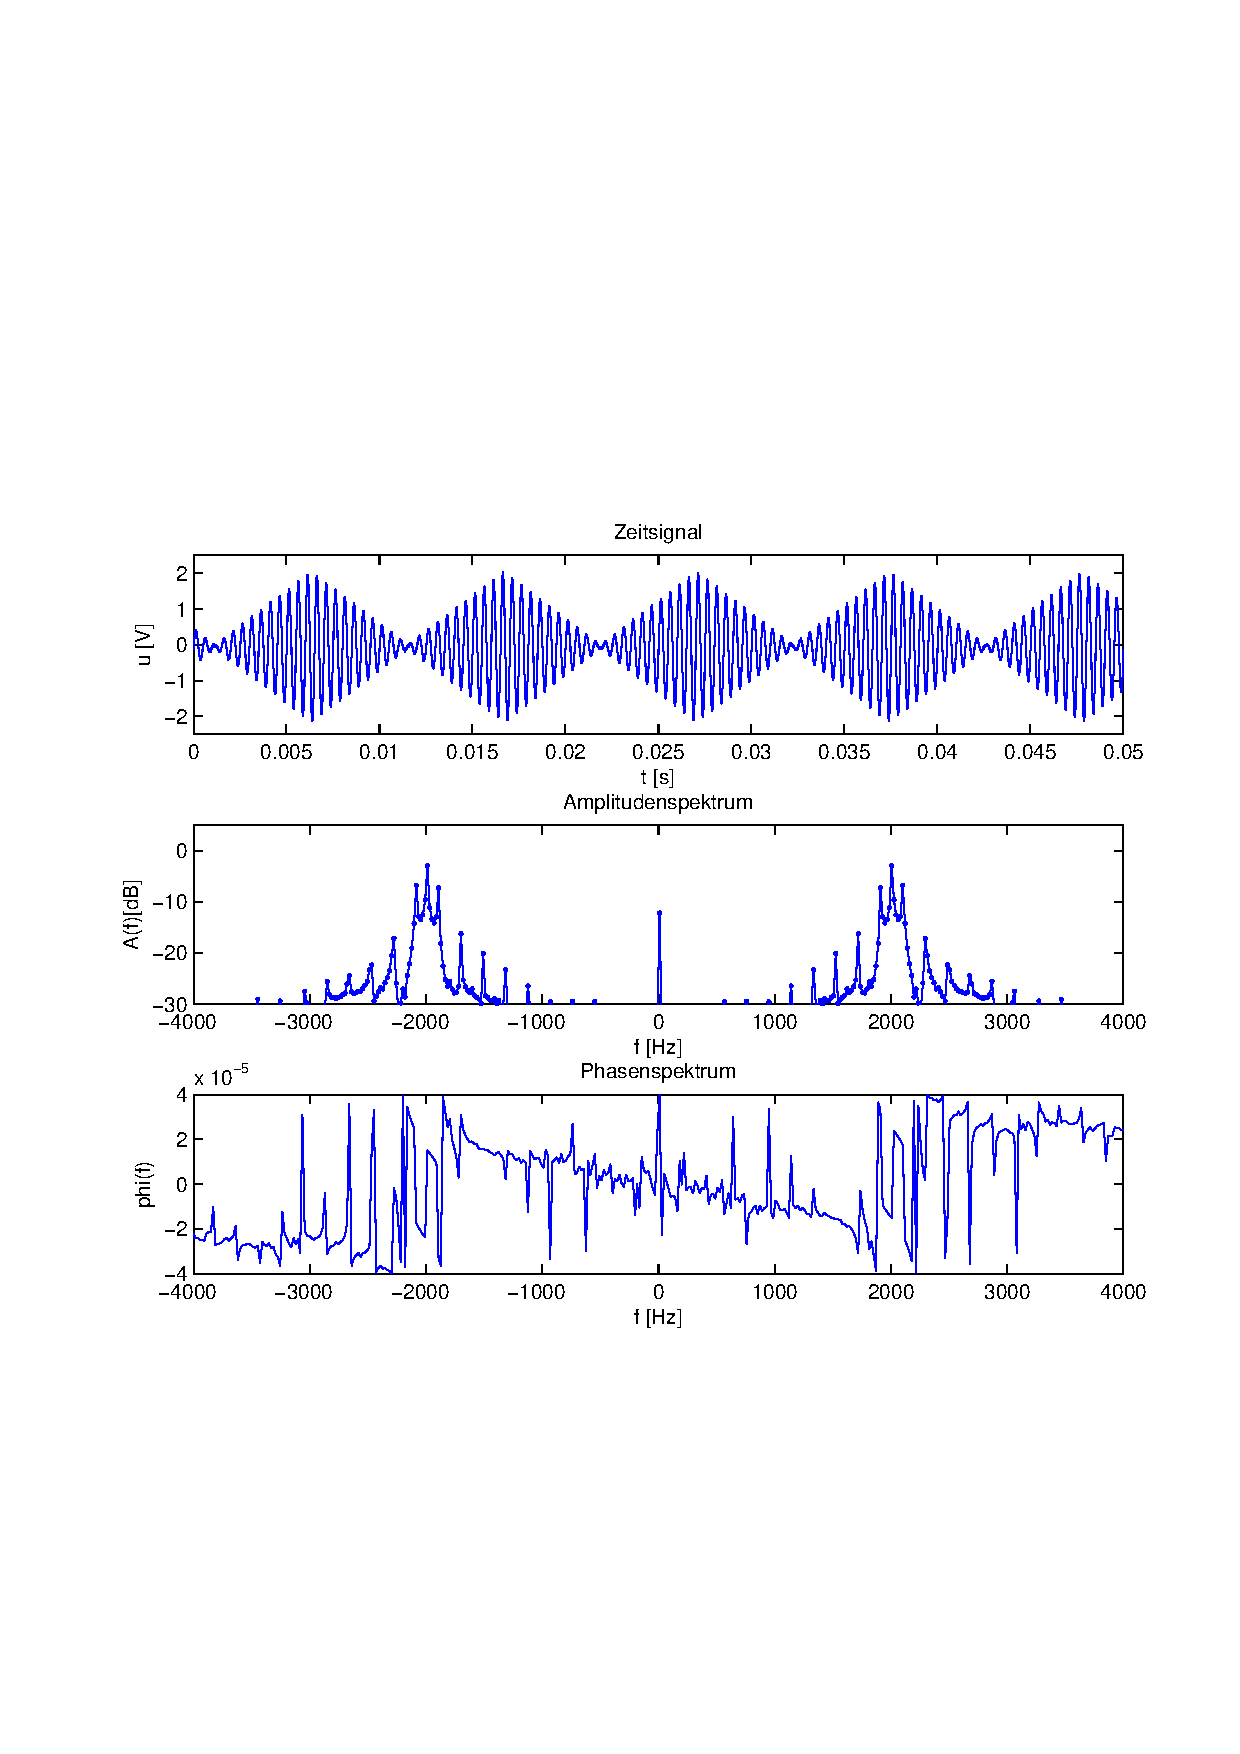
\includegraphics[scale=0.5, trim = 2cm 6.5cm 1.5cm
                        8.5cm, clip]{./Bilder/Dreieckmodgemessen} %FIXME
                        % [width=640px, height=474px]
                        \caption{amplitudenmoduliertes Dreiecksignal gemessen}
                    \end{figure}
               \vspace{-1.5em}

                \end{minipage}

            \end{tabular}
            \end{center}
            
                    \begin{center}
            \begin{tabular}{ll}

            \hspace{-10em}
                \begin{minipage}{0.6\textwidth}

                    \begin{figure}[H]
                        \label{fig:}
                        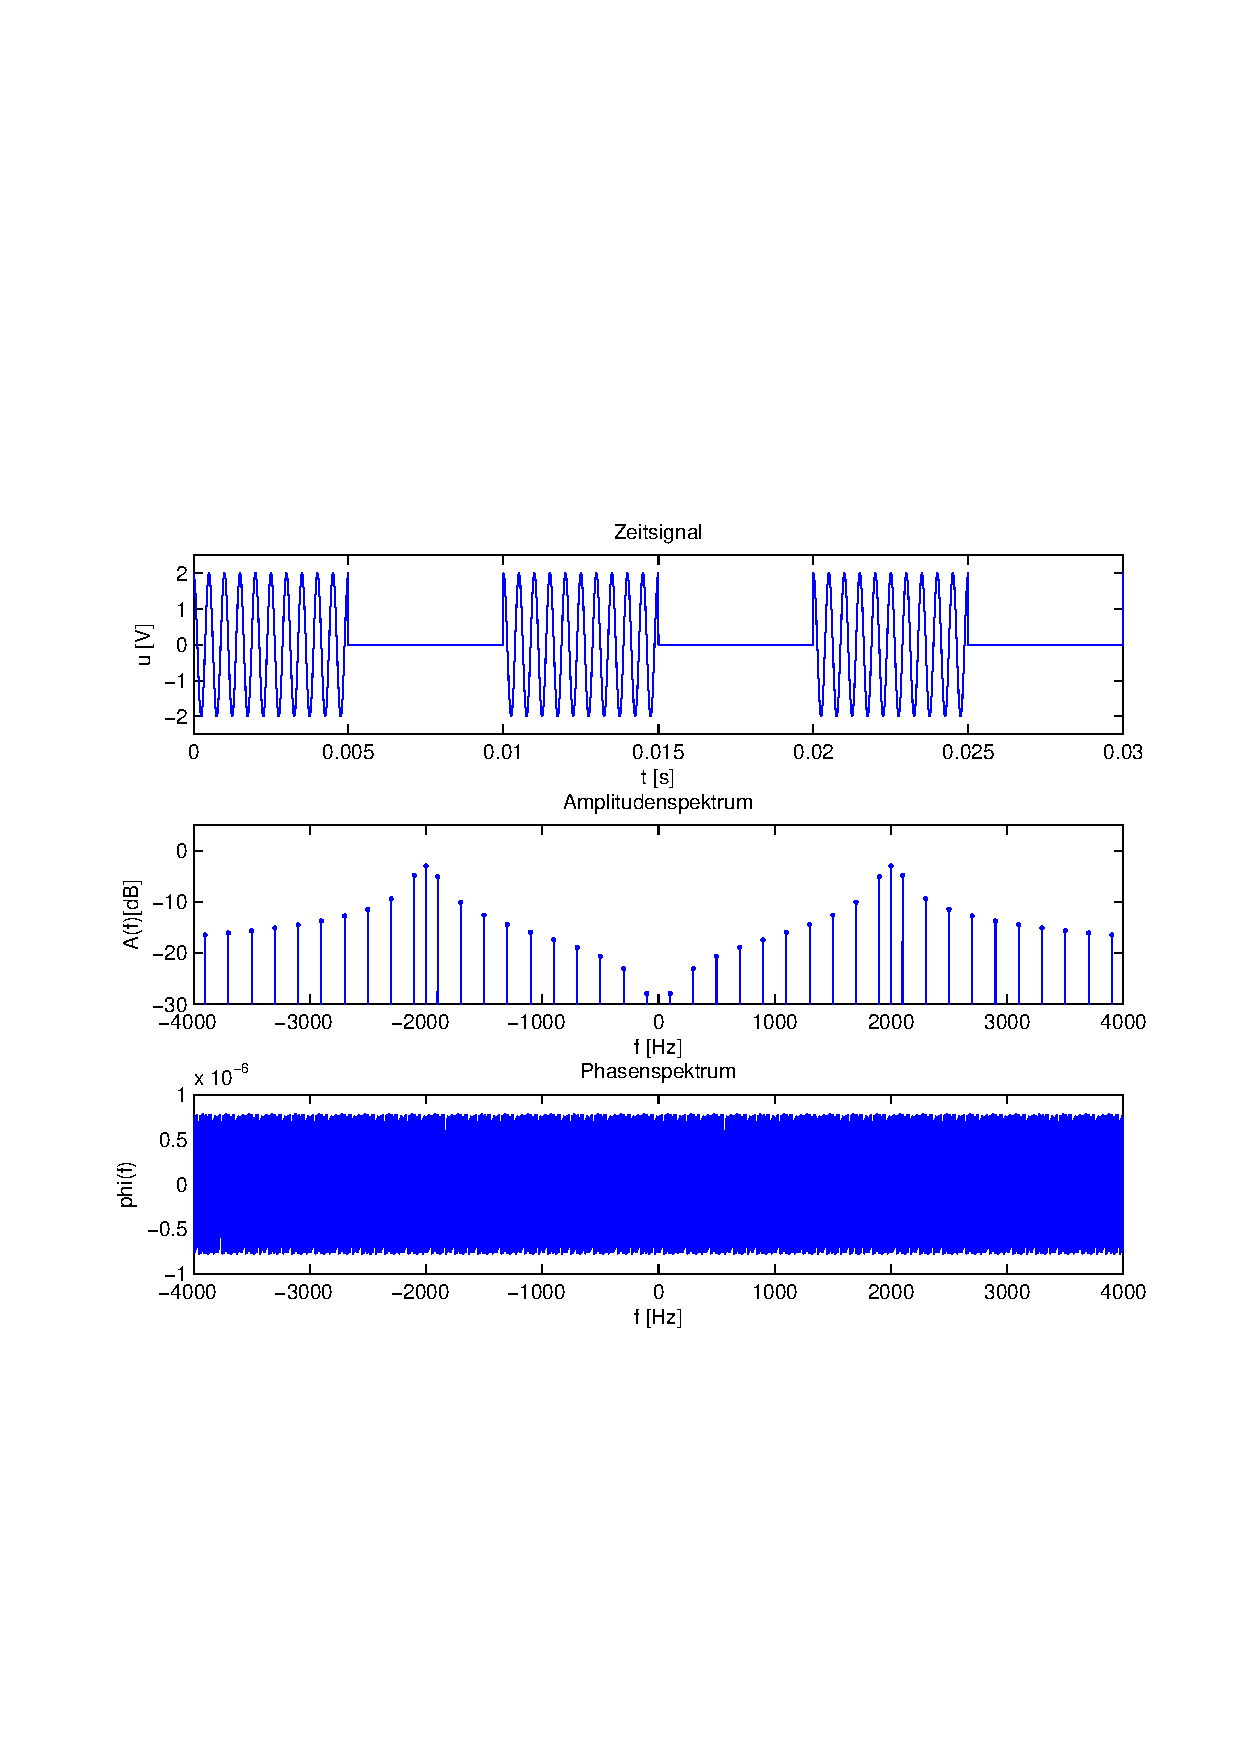
\includegraphics[scale=0.5, trim = 2cm 6.5cm 1.5cm
                        8.5cm, clip]{./Bilder/Rechteckmodsimuliert} %FIXME [width=640px,
                        % height=474px]
                        \caption{amplitudenmoduliertes Rechtecksignal simuliert}
                    \end{figure}

                \end{minipage}
                \begin{minipage}{0.6\textwidth}

                     \begin{figure}[H]
                        \label{fig:}
                        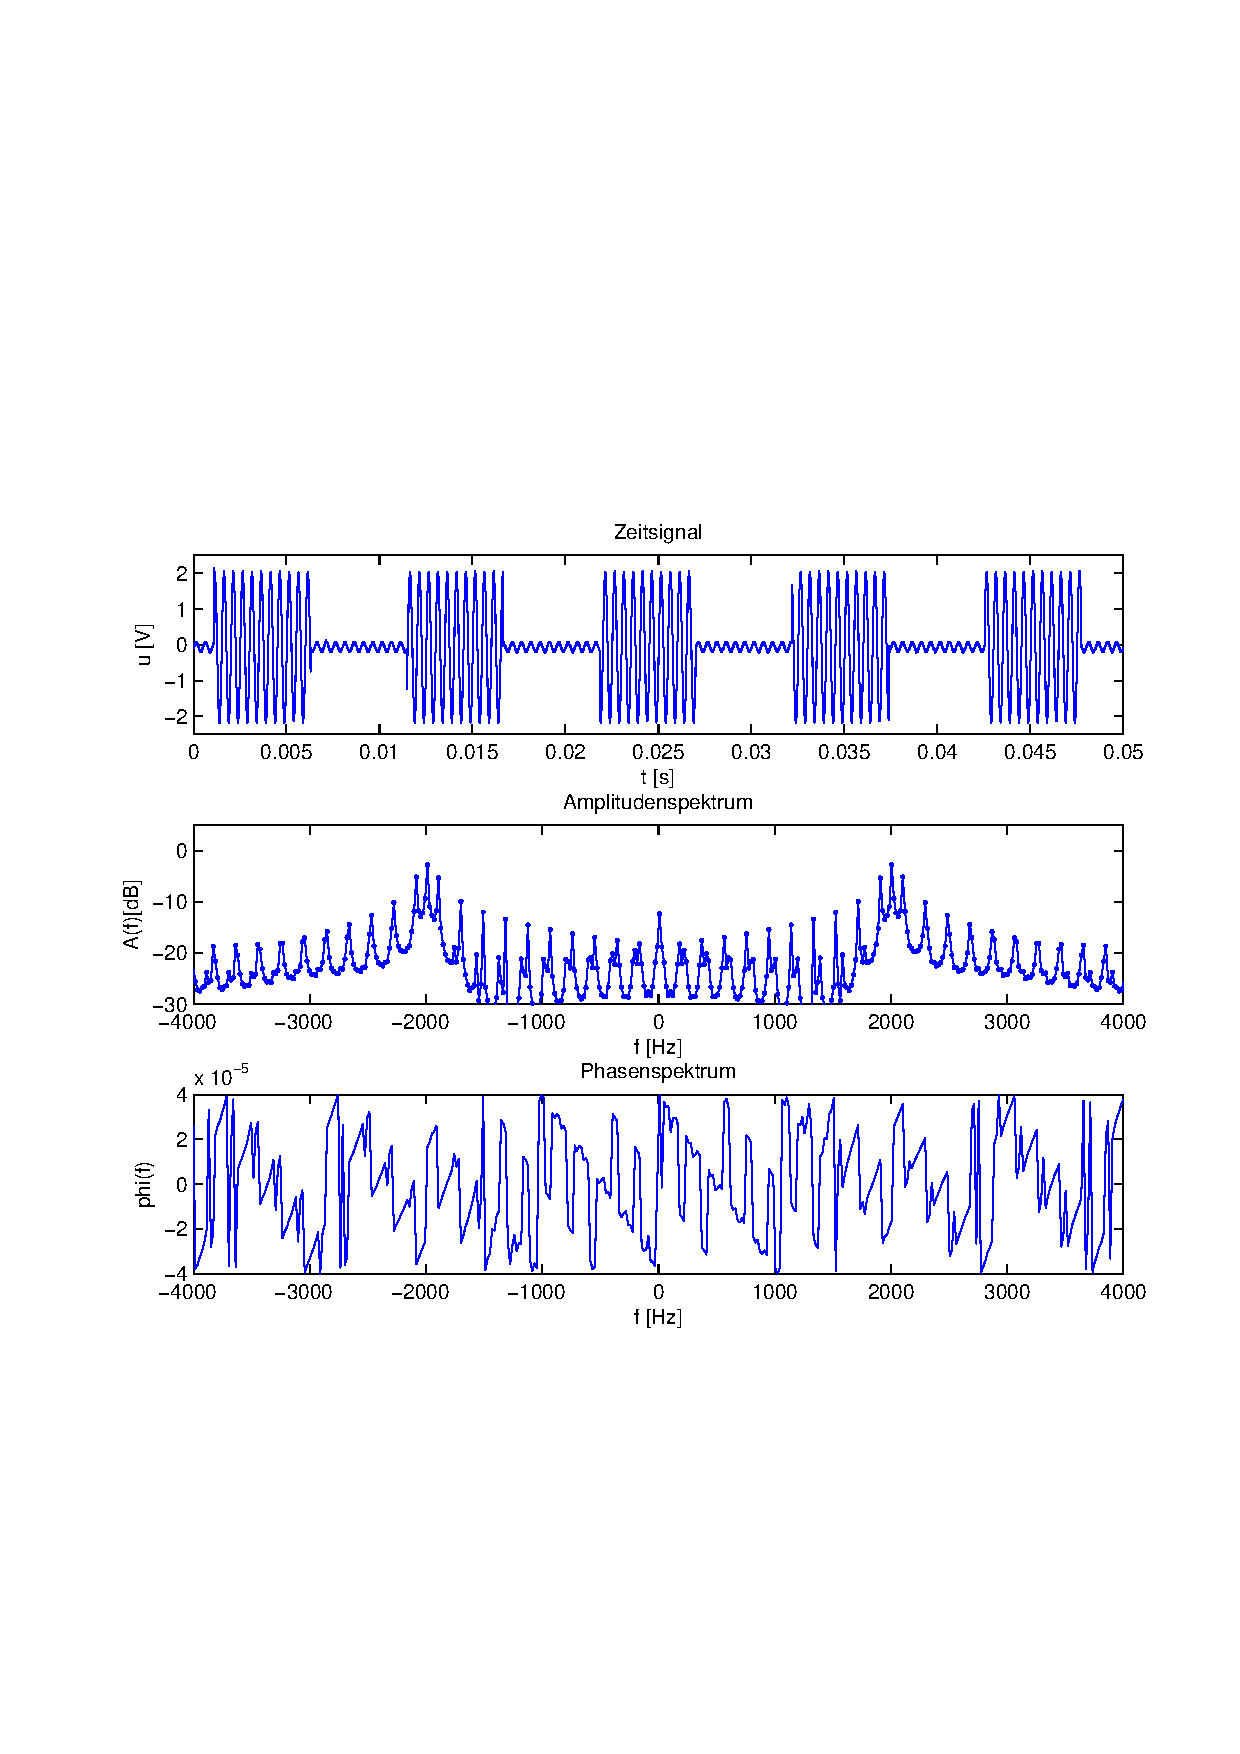
\includegraphics[scale=0.5, trim = 2cm 6.5cm 1.5cm
                        8.5cm, clip]{./Bilder/Rechteckmodgemessen} %FIXME
                        % [width=640px, height=474px]
                        \caption{amplitudenmoduliertes Rechtecksignal gemessen}
                    \end{figure}
               \vspace{-1.5em}

                \end{minipage}

            \end{tabular}
            \end{center}

        
        
        
        Bei der Demodulation wurde das Trägersignal auf das
        bereits modulierte Nutzsignal multipliziert. Die Synchronität war
        dadurch gewährleistet, dass das selbe Trägersignal wie bei der
        Modulation verwendet wurde.\\
        Hier werden die ursprünglichen Sendesignalen mit den
        demodulierten Empfangssignalen verglichen:
        
                \begin{center}
            \begin{tabular}{ll}

            \hspace{-14em}
                \begin{minipage}{0.6\textwidth}

                    \begin{figure}[H]
                        \label{fig:}
                        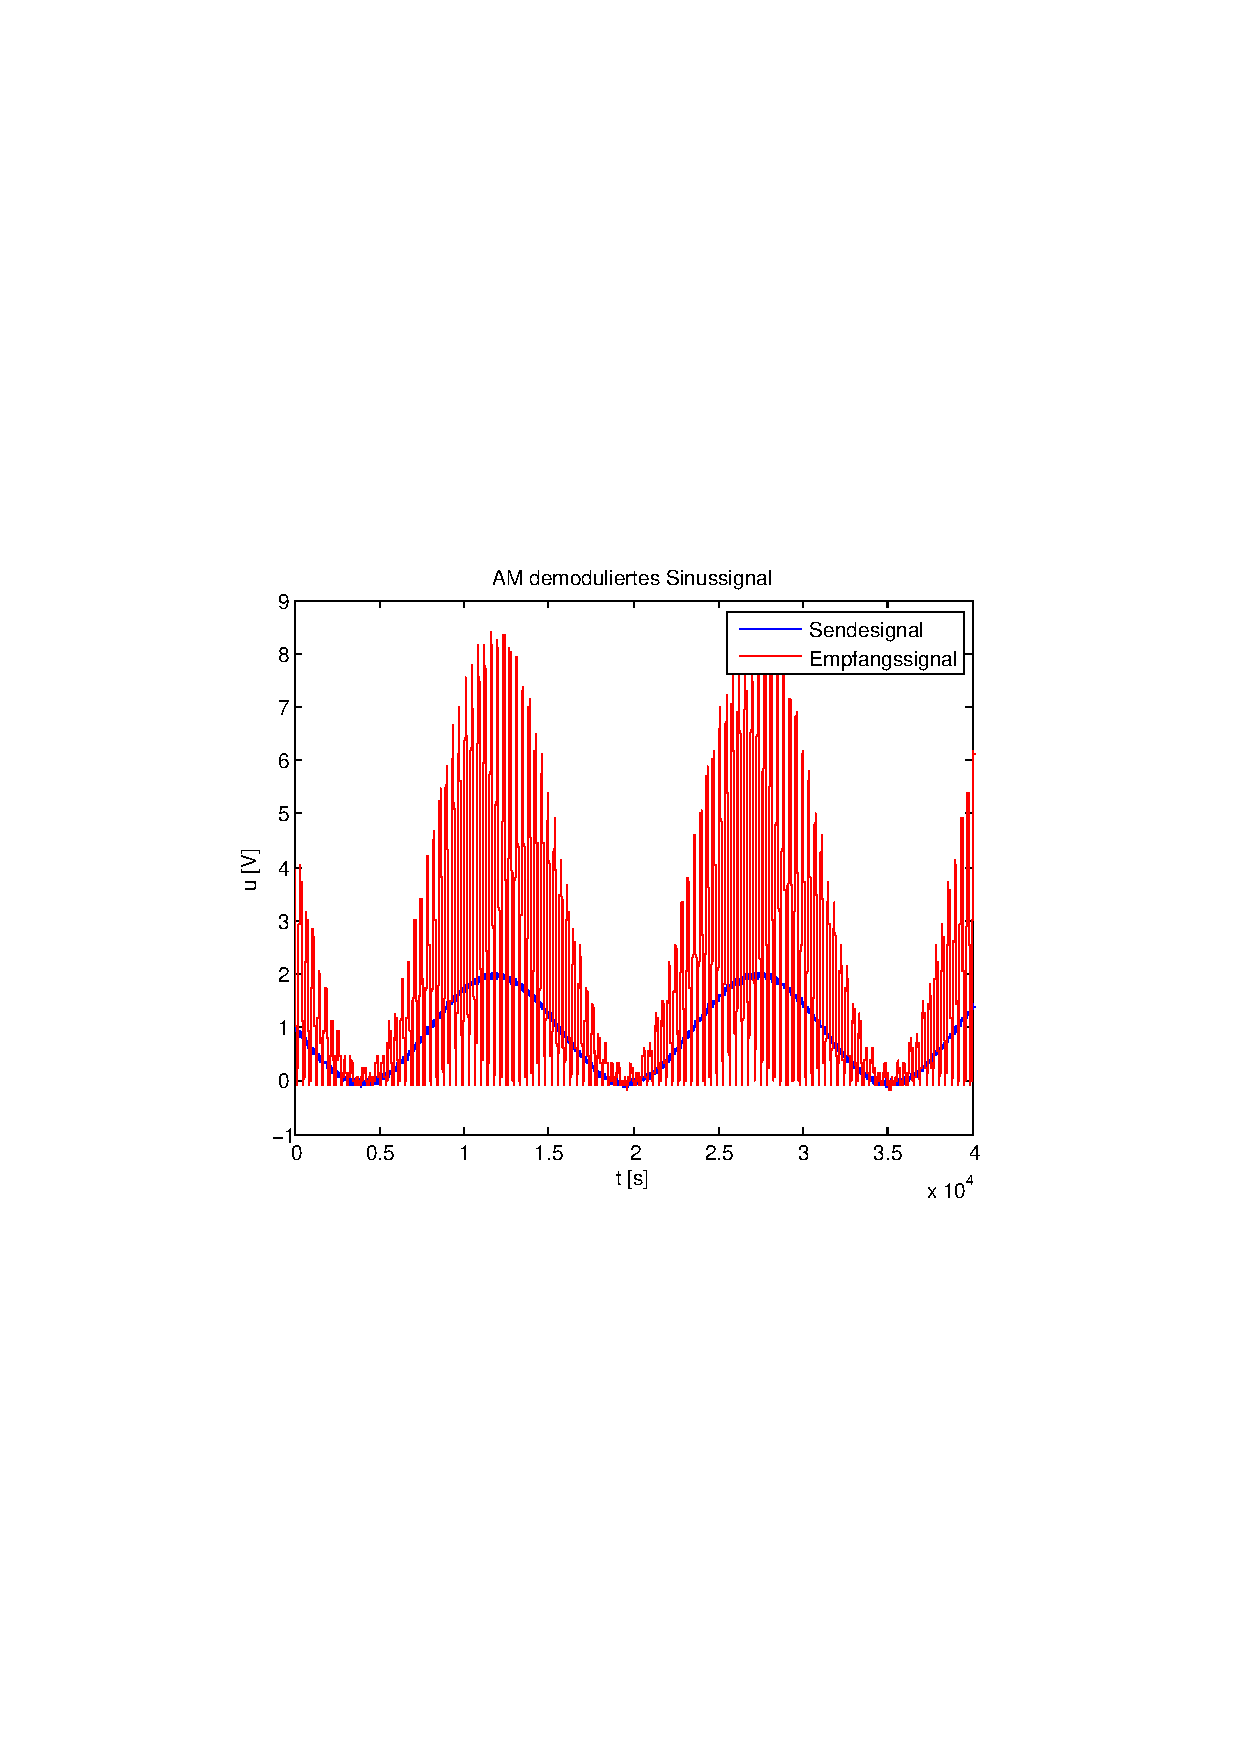
\includegraphics[scale=0.5, trim = 2cm 6.5cm 1.5cm
                        8.5cm, clip]{./Bilder/synchDemod_sinus} %FIXME
                        % [width=640px, height=474px]
                        \caption{amplitudendemoduliertes Sinussignal}
                    \end{figure}

                \end{minipage}
                \begin{minipage}{0.6\textwidth}

                     \begin{figure}[H]
                        \label{fig:}
                        \includegraphics[scale=0.5, trim = 2cm 6.5cm 1.5cm
                        8.5cm, clip]{./Bilder/synchDemod_dreieck} %FIXME
                        % [width=640px, height=474px]
                        \caption{amplitudendemoduliertes Dreiecksignal}
                    \end{figure}
               \vspace{-1.5em}

                \end{minipage}

            \end{tabular}
            \end{center}
            
             \begin{figure}[H] \centering
                    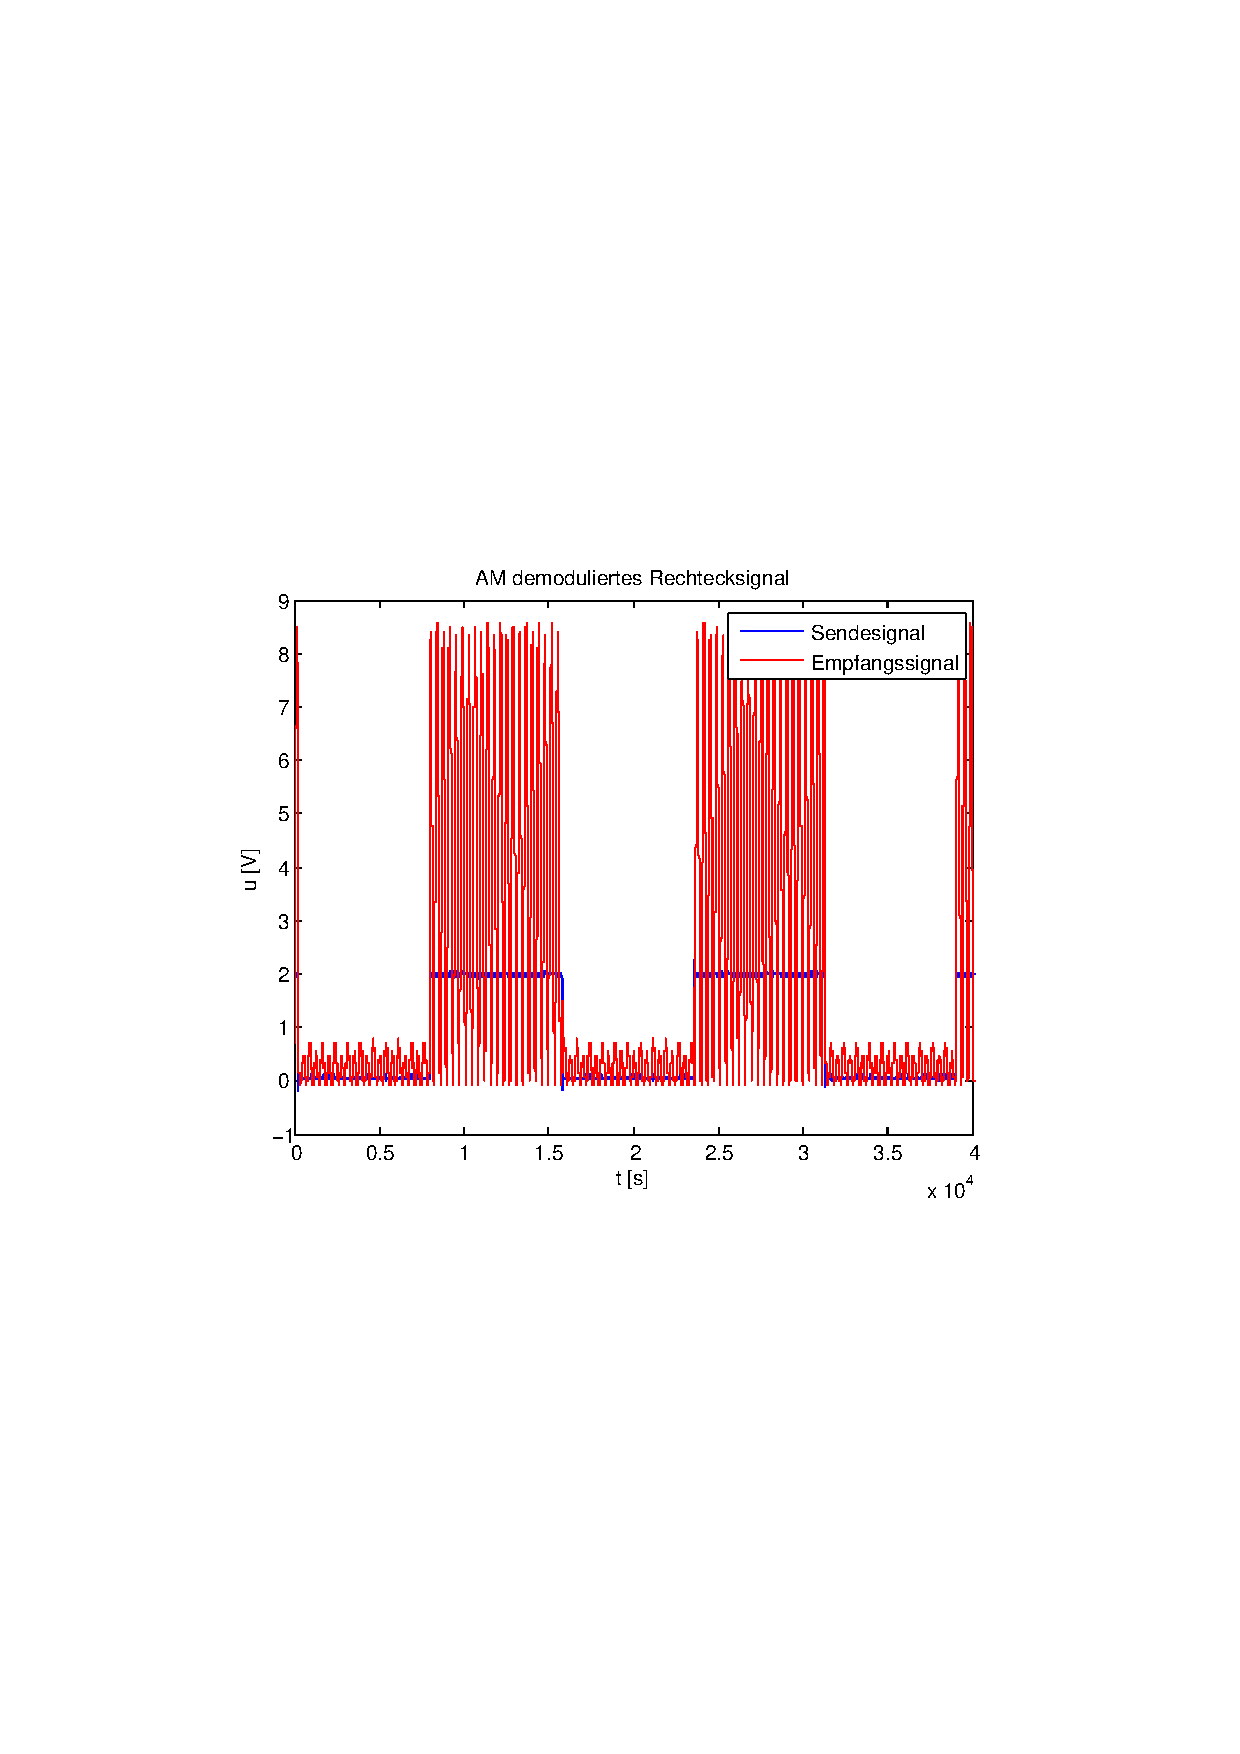
\includegraphics[scale=0.5, trim = 2cm 6.5cm 1.5cm 8.5cm,
                    clip]{./Bilder/synchDemod_rechteck}
                        \caption{amplitudendemoduliertes Rechtecksignal}
                \end{figure}
                
                Man kann deutlich sehen, dass die Amplituden der Empfangssignale
                stets um den Faktor $4$ höher sind als die Amplituden der
                Sendesignale. Dies liegt daran, dass \ldots
                
                Das noch fehlende Modul war ein Tiefpass, der auf dem
                Steckbrett bereits realisiert war, der die unnötig höheren
                Frequenzen filterte.
                Der TP wurde dabei manuell so eingestellt, bis das Ergebniss ungefähr 
                den Erwartungen des Sendesignals entsprach. Dabei maßen wir
                mithilfe des Oszilloskops die jeweiligen Periodendauer von den
                Empfangssignalen und konnten mit $T_{Periode}$ rückwirkend die
                Grenzfrequenzen bestimmen. Dabei verwendeten wir den
                Zusammenhang $f = \frac{1}{T}$. Wichtig dabei war es den in dem
                TP integrierten Vorfaktor von $100$ zu berücksichtigen, um keine 
                hundertfache Frequenzen zu erhalten. Es ergab sich für das
                Sinusempfangssignal eine Periode von $T = 50\mu s$ und die
                Grenzfrequenz $f = 0.2 kHz$. Für das Dreieckempfangssignal
                erhielten wir eine Periodendauer von $T = 20\mu s$ und die Grenzfrequenz
                $f = 0.5 kKz$ sowie eine Periodendauer von $T = 2.5\mu s$ und
                die Grenzfrequenz $f = 4 kKz$ für das Rechteckempfangssignal.
                Die Ergebnisse nach der Filterung wurden ebenfalls geplottet und
                erneut mit dem ursprünglichen Sendesignal verglichen.
                
                \begin{center}
            \begin{tabular}{ll}

            \hspace{-14em}
                \begin{minipage}{0.6\textwidth}

                    \begin{figure}[H]
                        \label{fig:}
                        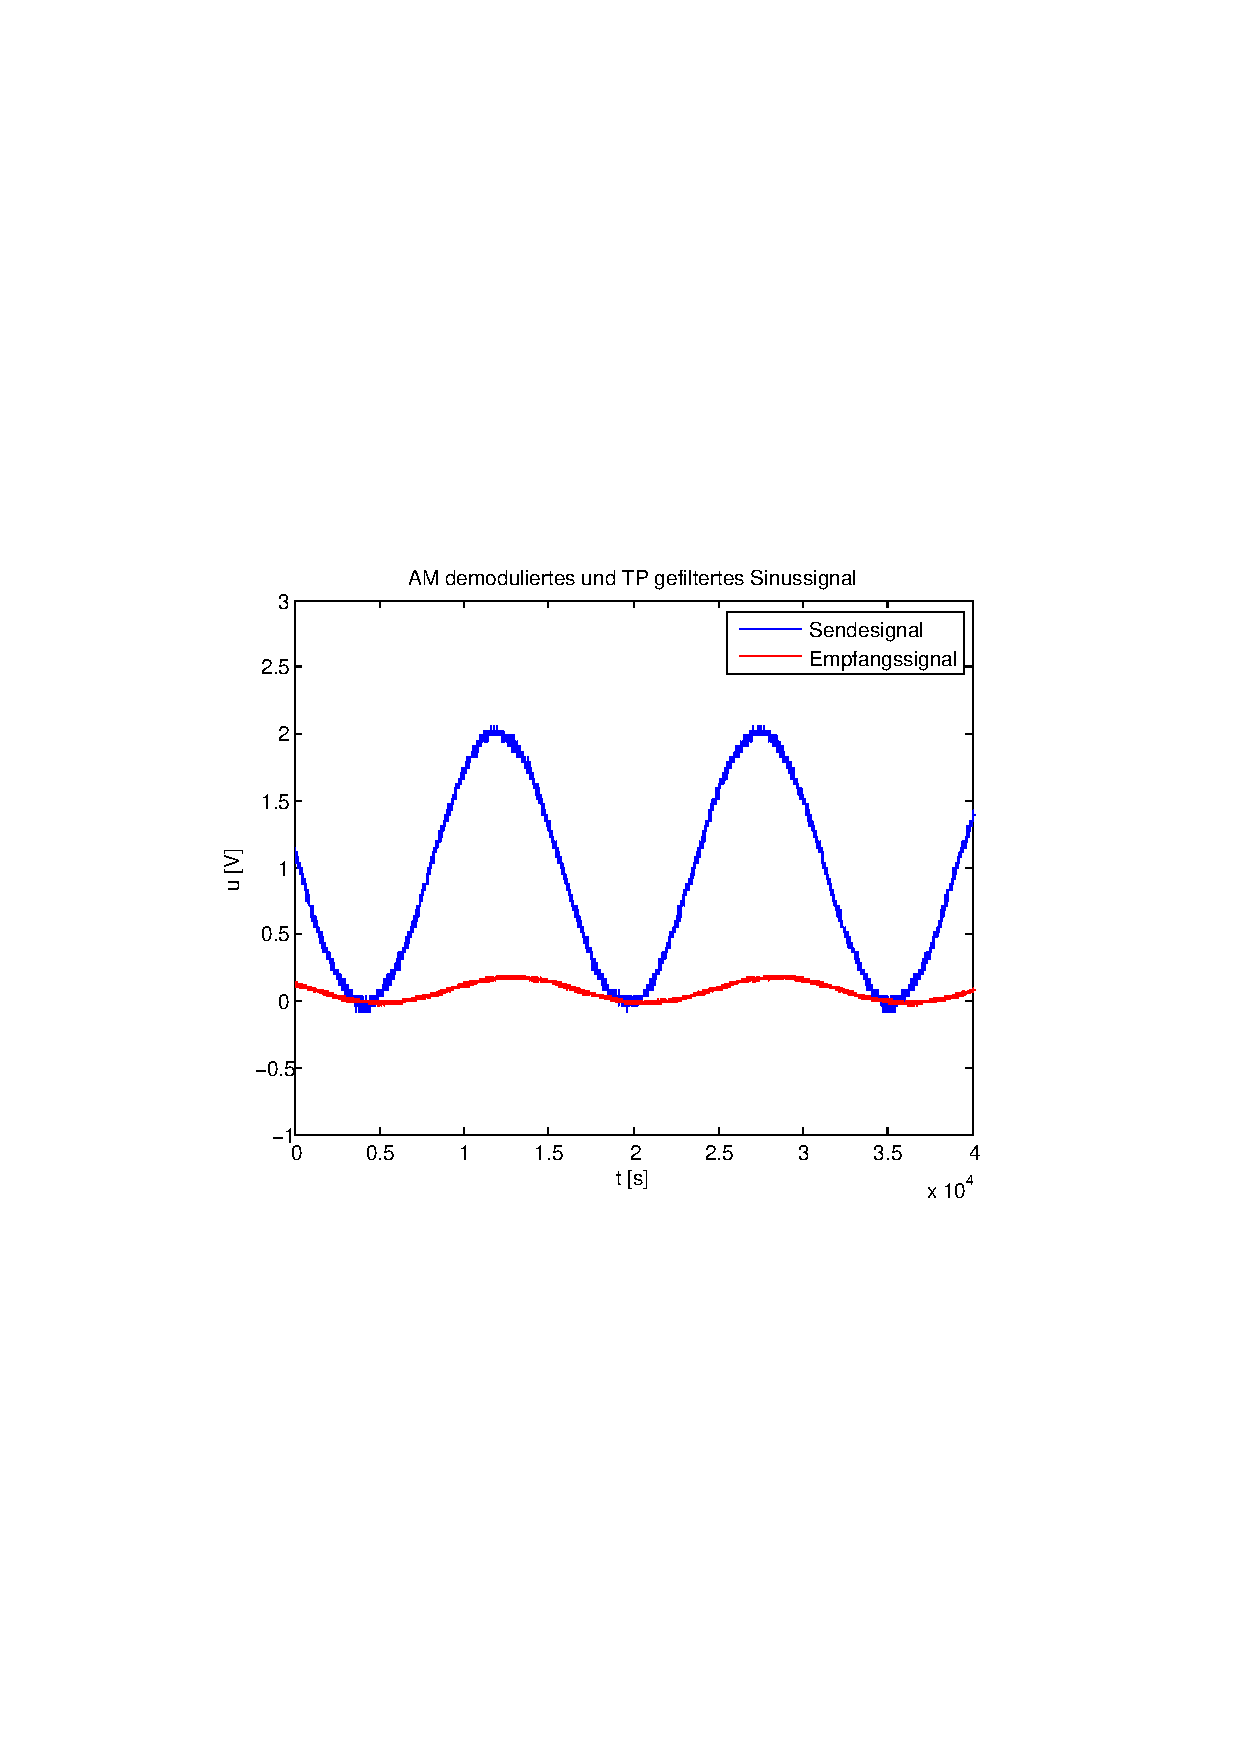
\includegraphics[scale=0.5, trim = 2cm 6.5cm 1.5cm
                        8.5cm, clip]{./Bilder/synchDemodFilter_sinus} %FIXME
                        % [width=640px, height=474px]
                        \caption{AM-demoduliertes und
                        TP-gefiltertes Sinussignal}
                    \end{figure}

                \end{minipage}
                \begin{minipage}{0.6\textwidth}

                     \begin{figure}[H]
                        \label{fig:}
                        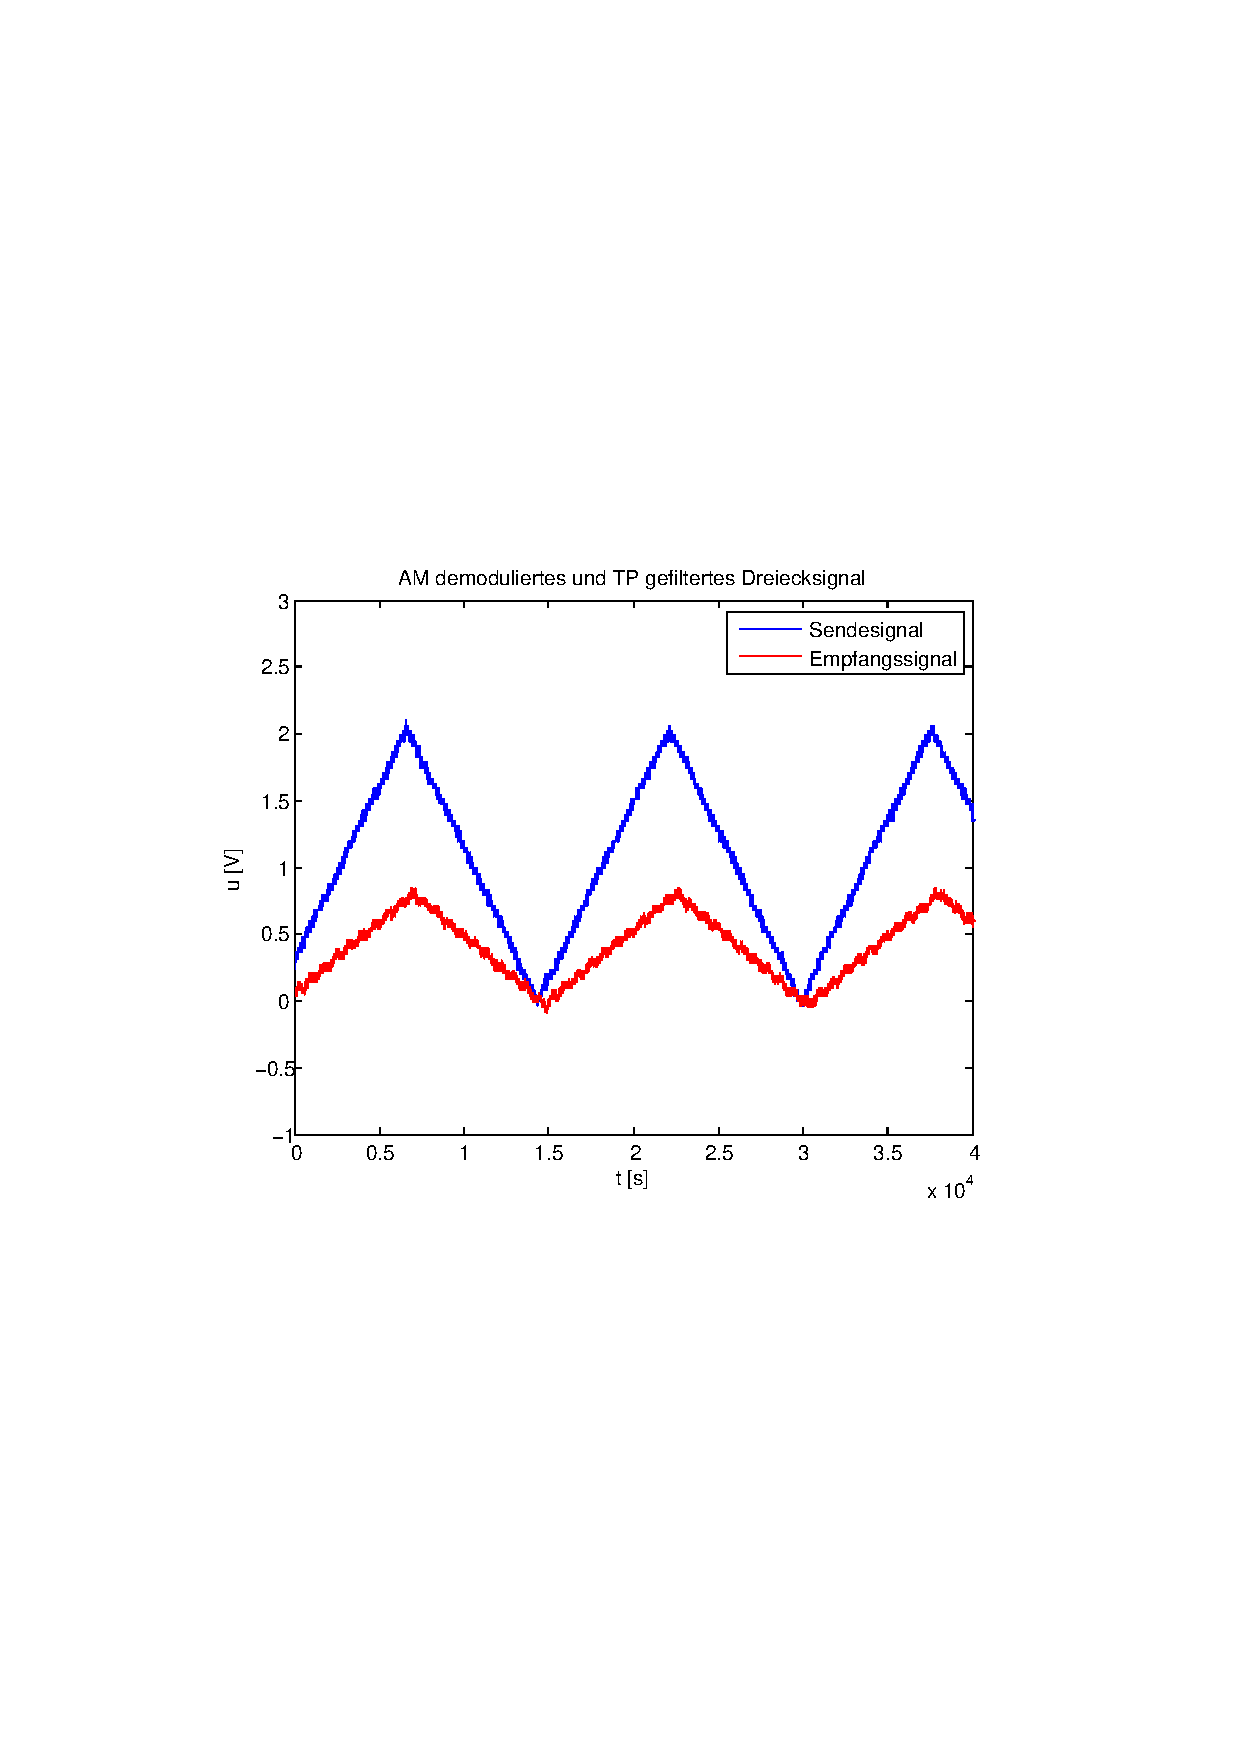
\includegraphics[scale=0.5, trim = 2cm 6.5cm 1.5cm
                        8.5cm, clip]{./Bilder/synchDemodFilter_dreieck} %FIXME
                        % [width=640px, height=474px]
                        \caption{AM-demoduliertes und
                        TP-gefiltertes Dreiecksignal}
                    \end{figure}
               \vspace{-1.5em}

                \end{minipage}

            \end{tabular}
            \end{center}
            
             \begin{figure}[H] \centering
                    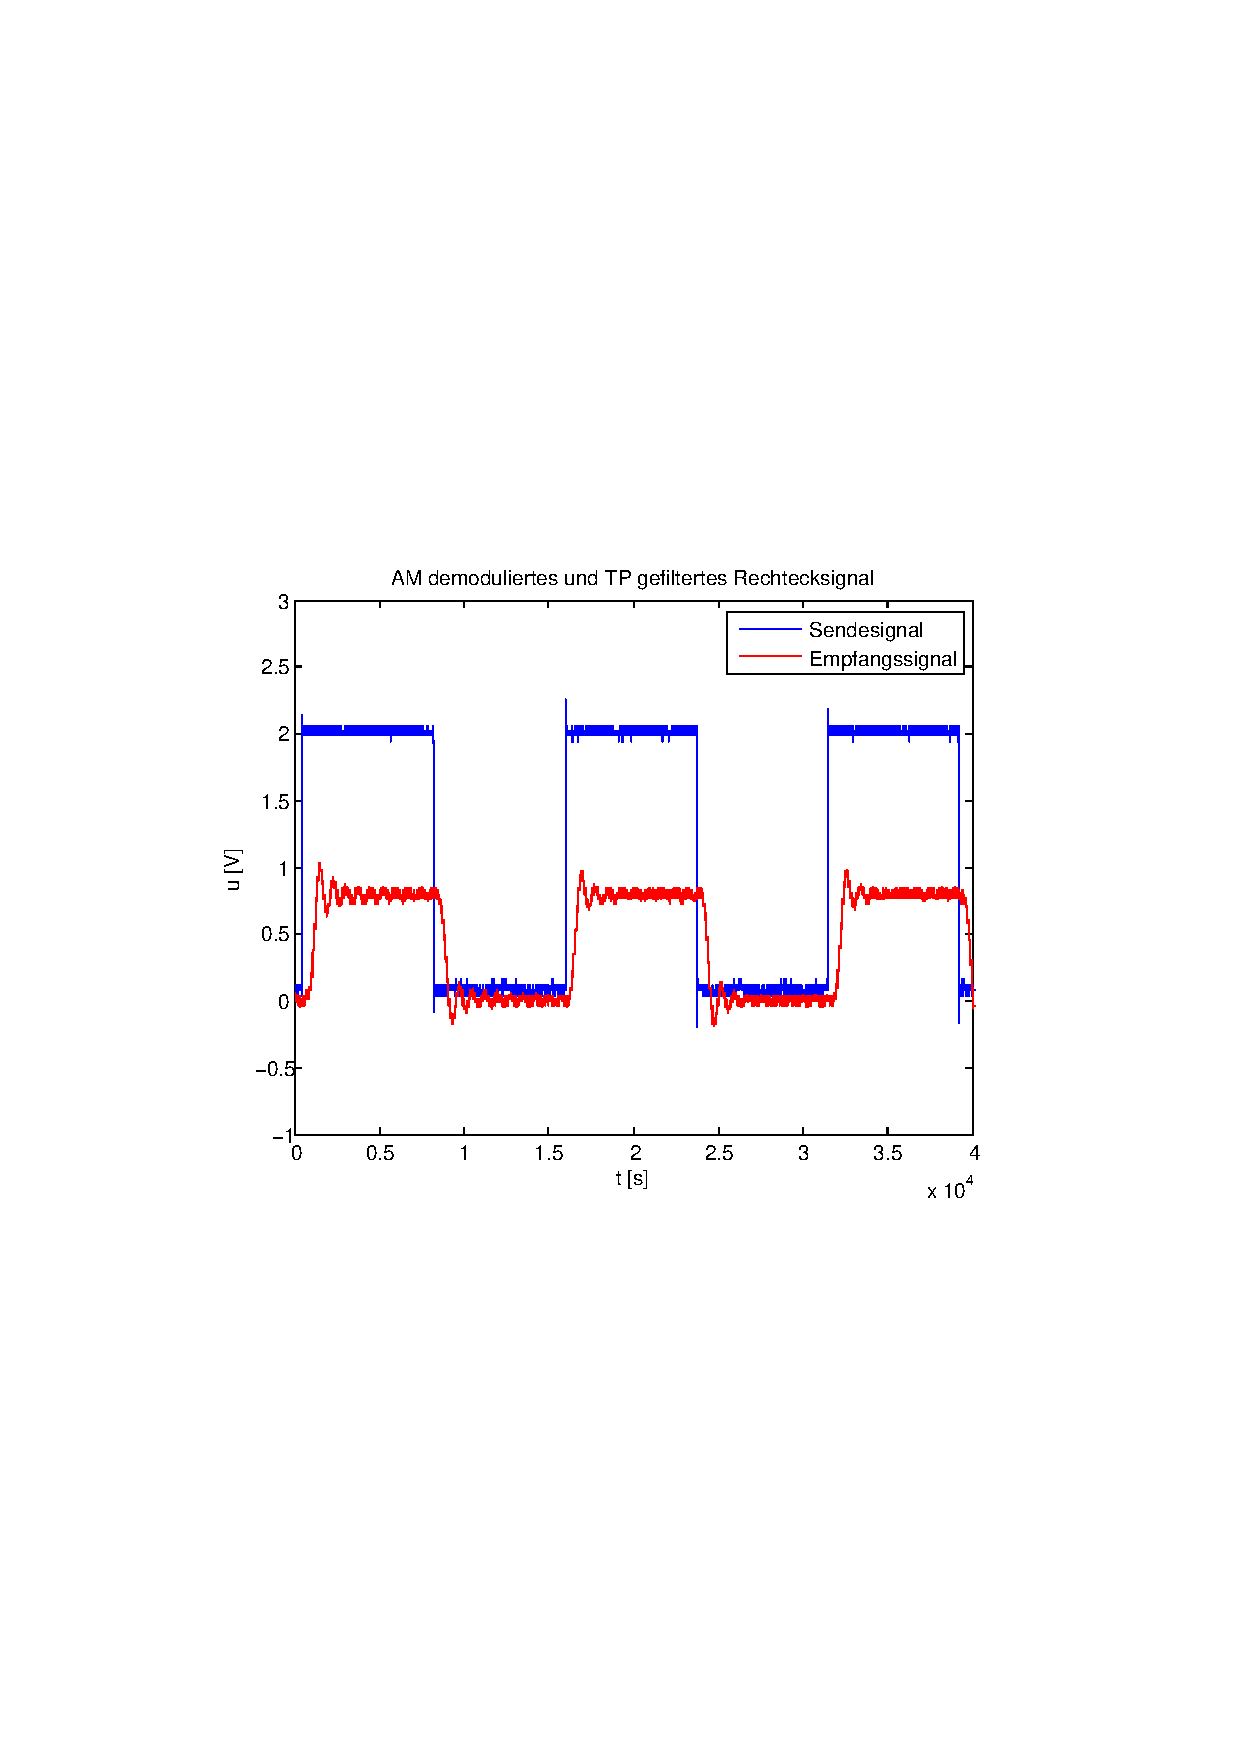
\includegraphics[scale=0.5, trim = 2cm 6.5cm 1.5cm 8.5cm,
                    clip]{./Bilder/synchDemodFilter_rechteck}
                        \caption{AM-demoduliertes und
                        TP-gefiltertes Rechtecksignal}
                \end{figure}
                
                Man kann nun sehen, dass die Amplituden der Empfangssignale
                deutlich kleiner sind als in der ungefilterten Demodulation,
                aber auch viel kleiner sind als die Amplituden Sendesignale.
                Die aufgetretenen Abweichungen kann man folgendermaßen erklären.
                
                Warum das so ist, weiß ich nicht mehr\ldots
                
                 
         
    \end{quote}
\end{quote}

%--------------------------------------------------------------------
%--------------------------------------------------------------------            



\section{Frequenzmodulation}
\begin{quote}
    \subsection{Theorie}
    \begin{quote}
        \TODO{Boris}
    \end{quote}
    
    \subsection{Vorbereitungsaufgabe}
    \begin{quote}
        Um ein Frequenzmoduliertes Signal zu simulieren, welches wir später mit einem gemessenen Signal zuvergleichen,
        erzeugen wir ein Cosinussignal mit einer Frequenz von $1kHz$ und einer Amplitude von $1V$. Anschließend
    \end{quote}
    
    \subsection{Durchführung}
    \begin{quote}
        \subsubsection{Signalerzeugung}
        \begin{quote}
        Als Nutzsignal für die Frequenzmodulation wird ein $3 kHz$-Sinus mit
        einer $1 V$-Amplitude verwendet. Die einfache Modulation verwirklichten
        wir anhand des VCO-Moduls. Dabei wurde der Schalter in der Mitte auf
        die Position LOW gesetzt (das Trägersignal kann damit eine
        Nutzsignalfrequenz zwischen $1 kHz$ und $17 kHz$ annehmbar modulieren),
        der FREQ-Controller auf die mittlere Position gestellt und GAIN auf
        $\approx \frac{2}{3}$ des Maximalwerts gedreht.\\
        Als nächstes wurde das Spektrum des FM-Signals untersucht und die
        Trägerfrequenz $f_c$ sowie die Proportionalitätskonstante $K_{FM}$
        bestimmt. Für die Proportionalitätskonstante gilf folgende Formel:
        
        \begin{equation*}
    	\begin{split}
    		K_{FM} &= \frac{2 \pi \Delta f_{max}}{A_u}\\
			\Delta f_{max} \approx \frac{1}{2} (\frac{1}{T_{min}} - \frac{1}{T_{max}})    		
    	\end{split}
    	\end{equation*}
    	
   		$T_{min}$ und $T_{max}$ bezeichnen dabei die zeitlich kürzeste und längste
   		Periodendauer des Sinussignals.\\
   		Für einen späteren Vergleich wird auch das Spektrum des FM-Signals
   		untersucht, bei der die Nutzfrequenz $f_u = 1 kHz$ und die Nutzamplitude
   		$A_u = 1 V$ beträgt.\\
   		Zusätzlich wurden noch die Nutzsignale mit den Amplituden $0.5 V\, 1 V$ und
   		$2 V$ mit den Frequenzen $50 Hz\, 100 Hz$ und $200 Hz$ frequenzmoduliert
   		und die Spektren des Ausgangs von dem VCO-Modul miteinander verglichen. 
        \end{quote}
        
        \subsubsection{FM-Demodulation}
        \begin{quote}
        Für die folgende FM-Demodulation wurde zunächst die Einstellungen des
        VCO-Moduls verändert. Der Schalter wurde auf HIGH gelegt (nun kann das
        Trägersignal höhere Nutzfrequenzen als $17 kHz$ modulieren), sowie der
        Trägerfrequenz-Drehknopf auf die Hälfte und der GAIN-Drehknopf auf $70
        \%$ eingestellt. Das neu FM-modulierte Sinussignal, mit ursprünglich
        $100 Hz$-Frequenz und $1 V$-Amplitude, wurde dann auf den Eingang des
        Comparator-Moduls gelegt und mit einer Referenzspannung von $0 V$
        verglichen.\\
        
        Die FM-Demodulation erfolgt in diesem Praktikum durch eine
        FM-PFM-Umwandlung (PFM = Pulsfrequenzmodulation). Dabei wandelt der
        Comparator das analoge Signal in ein Standard-Digitalsignal um. Dieses
        besteht aus einer polaren Rechteckfolge, welche dadurch entsteht, dass
        der Comparator jedesmal, wenn das Analogsignal (in diesem Fall der
        von uns verwendete Sinus) das Referenzsignal übersteigt, einen positiven
        Ausgangssignalpegel ausgibt. Wird das Analogsignal kleiner als die
        Referenzspannung wird der Ausgangssignalpegel negativ. Dieses digitale
        Signal wird in den Twin Pulse Generator (TPG) geführt, der aus jeder
        steigenden Flanke ein Rechteckimpuls verwirklicht. Dafür werden die
        Regler DELAY und WIDTH auf ihr Minimum gedreht. Die Pulse des
        entstandenen Rechtecksignals werden abschließend wieder zu einem kontinuierlichen 
        Signalpegel umgewandelt, indem sie durch einen Tiefpass
        (TP) geführt werden.\\
        
        In der Auswertung vergleichen wir zusätzlich die das Sinusquellsignal
        mit dem Comparator-Ausgang, das Sinusquellsignal mit dem Twin Pulse
        Generator-Ausgang und den Comparator-Ausgang mit dem Twin Pulse
        Generator-Ausgang.
         
        \end{quote}
        
    \end{quote}
    
    \subsection{Auswertung}
    \begin{quote}
    
        Nach der Frequenzmodulation des Sinusnutzsignals mit der Frequenz 
        $3 kHz$ und der Amplitude $1 V$ erhielten wir folgendes Zeitsignal.
    	
             \begin{figure}[H] \centering
                    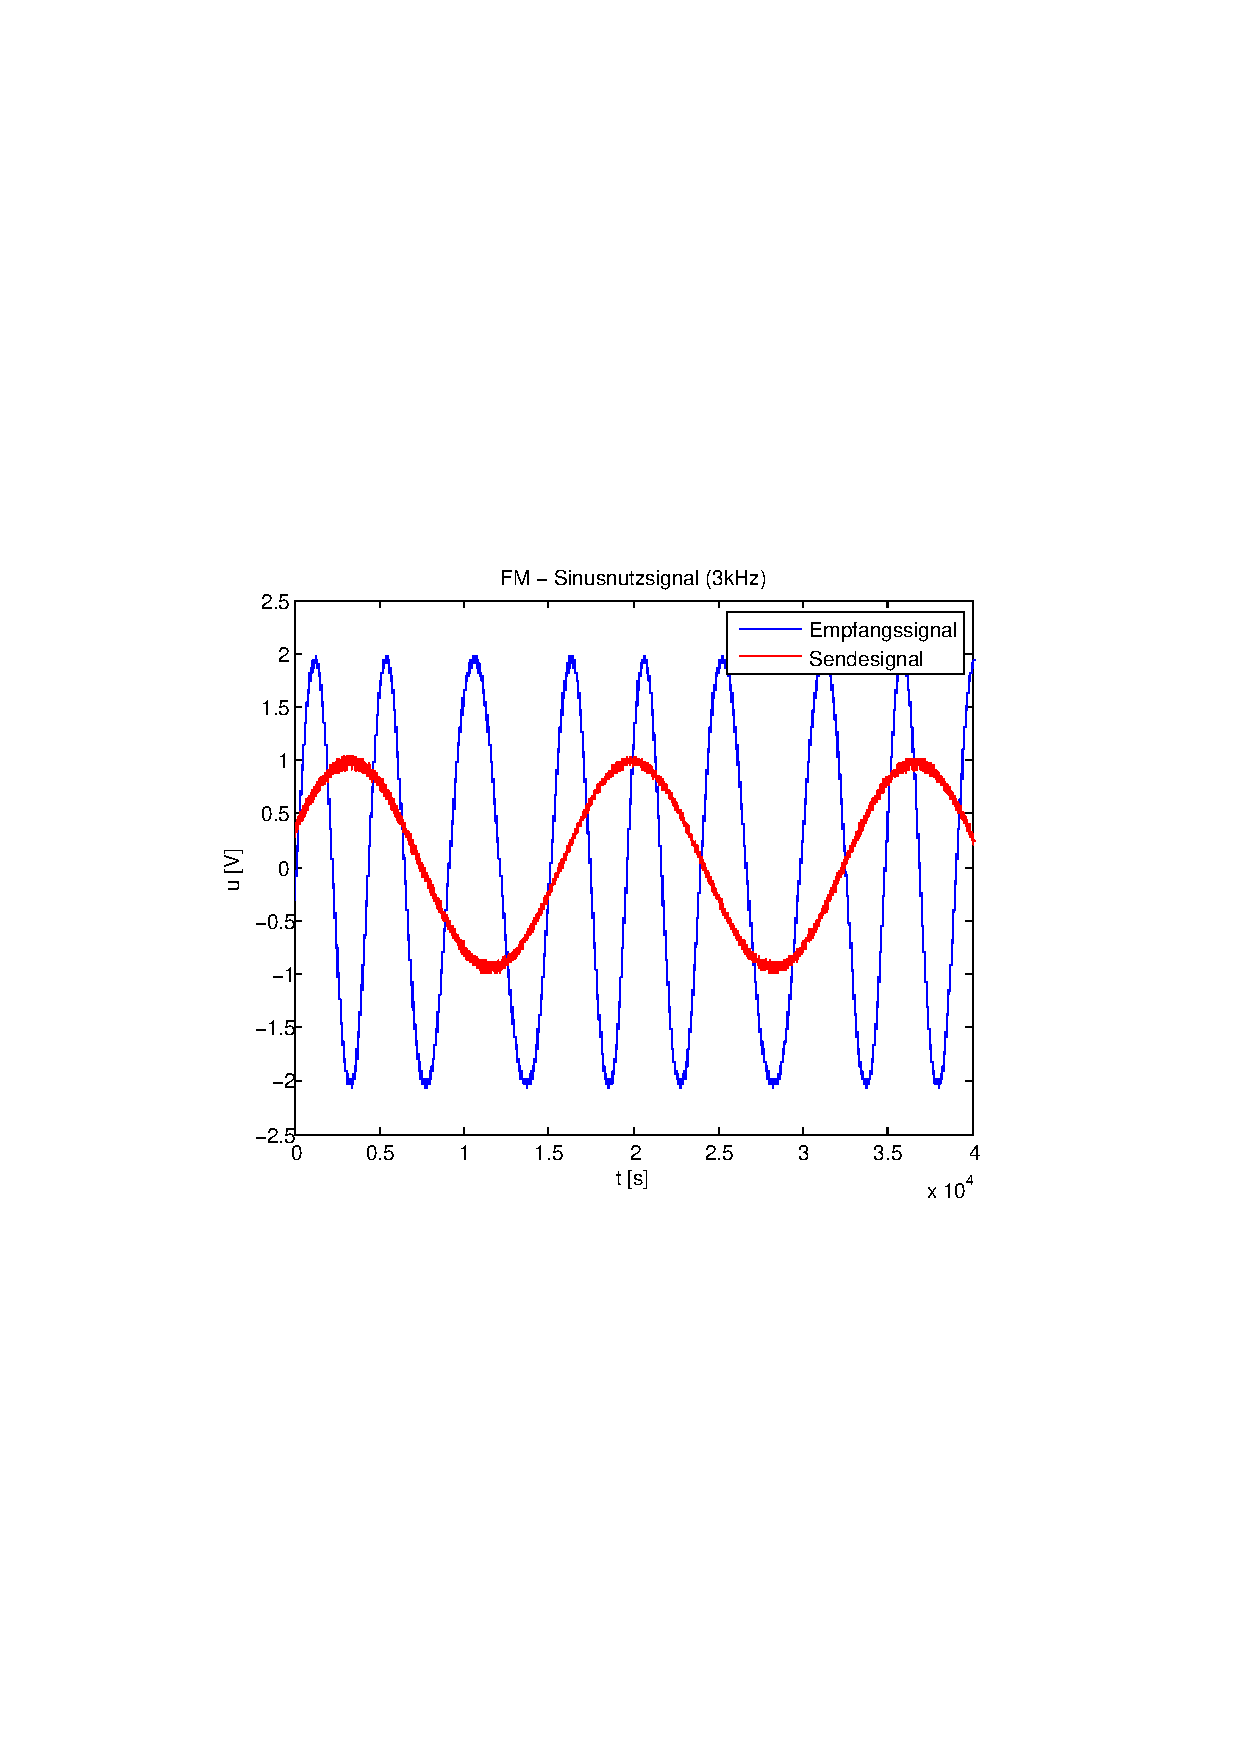
\includegraphics[scale=0.5, trim = 2cm 6.5cm 1.5cm 8.5cm,
                    clip]{./Bilder/fm_sinus(3kHz)}
                        \caption{frequenzmoduliertes Sinusnutzsignal (3kHz)}
                \end{figure}
        
        Das Verhältnis dieser beiden Signale wurde mit dem Oszilloskop genauer
        untersucht um die Proportionalitätskonstante berechnen zu können. Dafür
        zoomten wir einmal in einen passenden Bereich, wo die Amplitude des
        Nutzsignals hoch war und einmal in einen passenden Bereich, wo die
        Amplitude des Nutzsignals niedrig war.
        
         
                \begin{center}
            \begin{tabular}{ll}

            \hspace{-14em}
                \begin{minipage}{0.6\textwidth}

                    \begin{figure}[H]
                        \label{fig:}
                        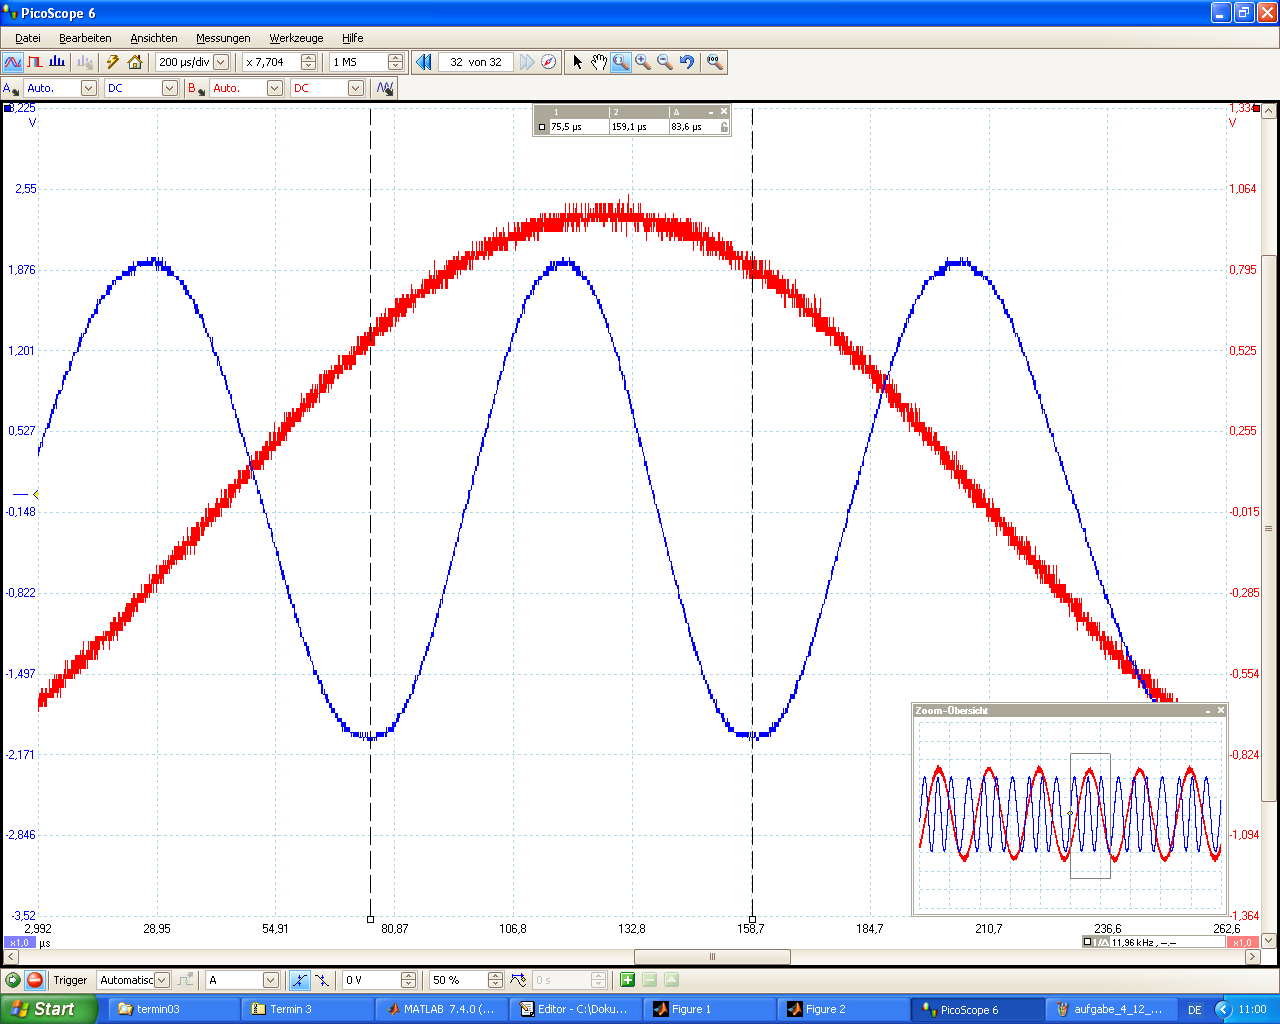
\includegraphics[scale=0.5, trim = 2cm 6.5cm 1.5cm
                        8.5cm, clip]{./Bilder/aufgabe_4_12_sinus_high-ampl}
                        %FIXME [width=640px, height=474px]
                        \caption{hohe Amplitude des Nutzsignals zur
                        Periodendauerbestimmung (Tmin) des FM-Empfangssignals}
                    \end{figure}

                \end{minipage}
                \begin{minipage}{0.6\textwidth}

                     \begin{figure}[H]
                        \label{fig:}
                        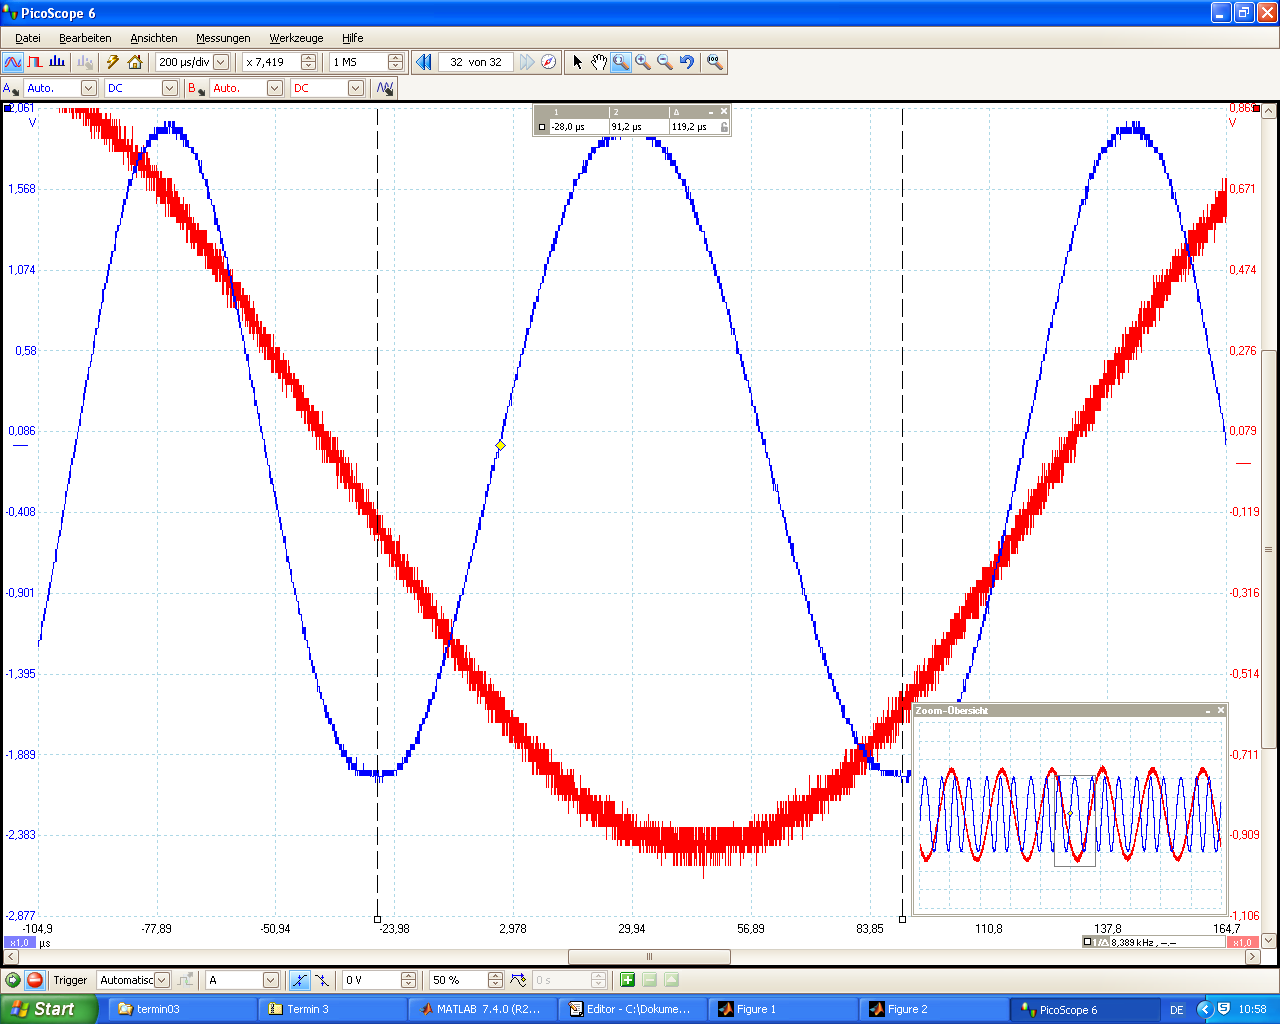
\includegraphics[scale=0.5, trim = 2cm 6.5cm 1.5cm
                        8.5cm, clip]{./Bilder/aufgabe_4_12_sinus_low-ampl}
                        %FIXME [width=640px, height=474px]
                        \caption{niedrige Amplitude des Nutzsignals zur
                        Periodendauerbestimmung (Tmax) des FM-Empfangssignals}
                    \end{figure}
               \vspace{-1.5em}

                \end{minipage}

            \end{tabular}
            \end{center}
        
        Bei der ersten Messung erhielten wir eine $T_{min}$ von ungefähr 
        $84\mu s$, bei der zweiten Messung waren es für $T_{max}$ ungefähr 
        $120\mu s$. Mit diesen Werten können wir zunächst das $\Delta f_{max}$
        berechnen, womit dich dann auch das $K_{FM}$ (mit $A_u = 1V$) berechnen
        lässt.
        
      \begin{equation*}
       \begin{split}
		\Delta f_{max} &\approx \frac{1}{2} (\frac{1}{84\mu s} - \frac{1}{120\mu s})\\
					   &\approx 1.786 kHz \\
		\\			
			
	    K_{FM} &= \frac{2 \pi \cdot 1.786 kHz}{1 V}\\
	    	   &= 11221.768    		
       \end{split}
     \end{equation*}
        
        Somit beträgt unser Proportionalitätsfaktor $K_{FM} = 11221.768$.\\
        
        Für die Berechnung der Trägerfrequenz wird folgendes getan\ldots 
        (müssen wir auf jeden Fall noch ergänzen) 
        
        Um einen Vergleich anstellen zu können, wurde auch das Spektrum des
        Sinussignals mit $1 kHz$ Frequenz aufgenommen. Die Ergebnisse folgen
        hier:
        
                \begin{center}
            \begin{tabular}{ll}

            \hspace{-14em}
                \begin{minipage}{0.6\textwidth}

                    \begin{figure}[H]
                        \label{fig:}
                        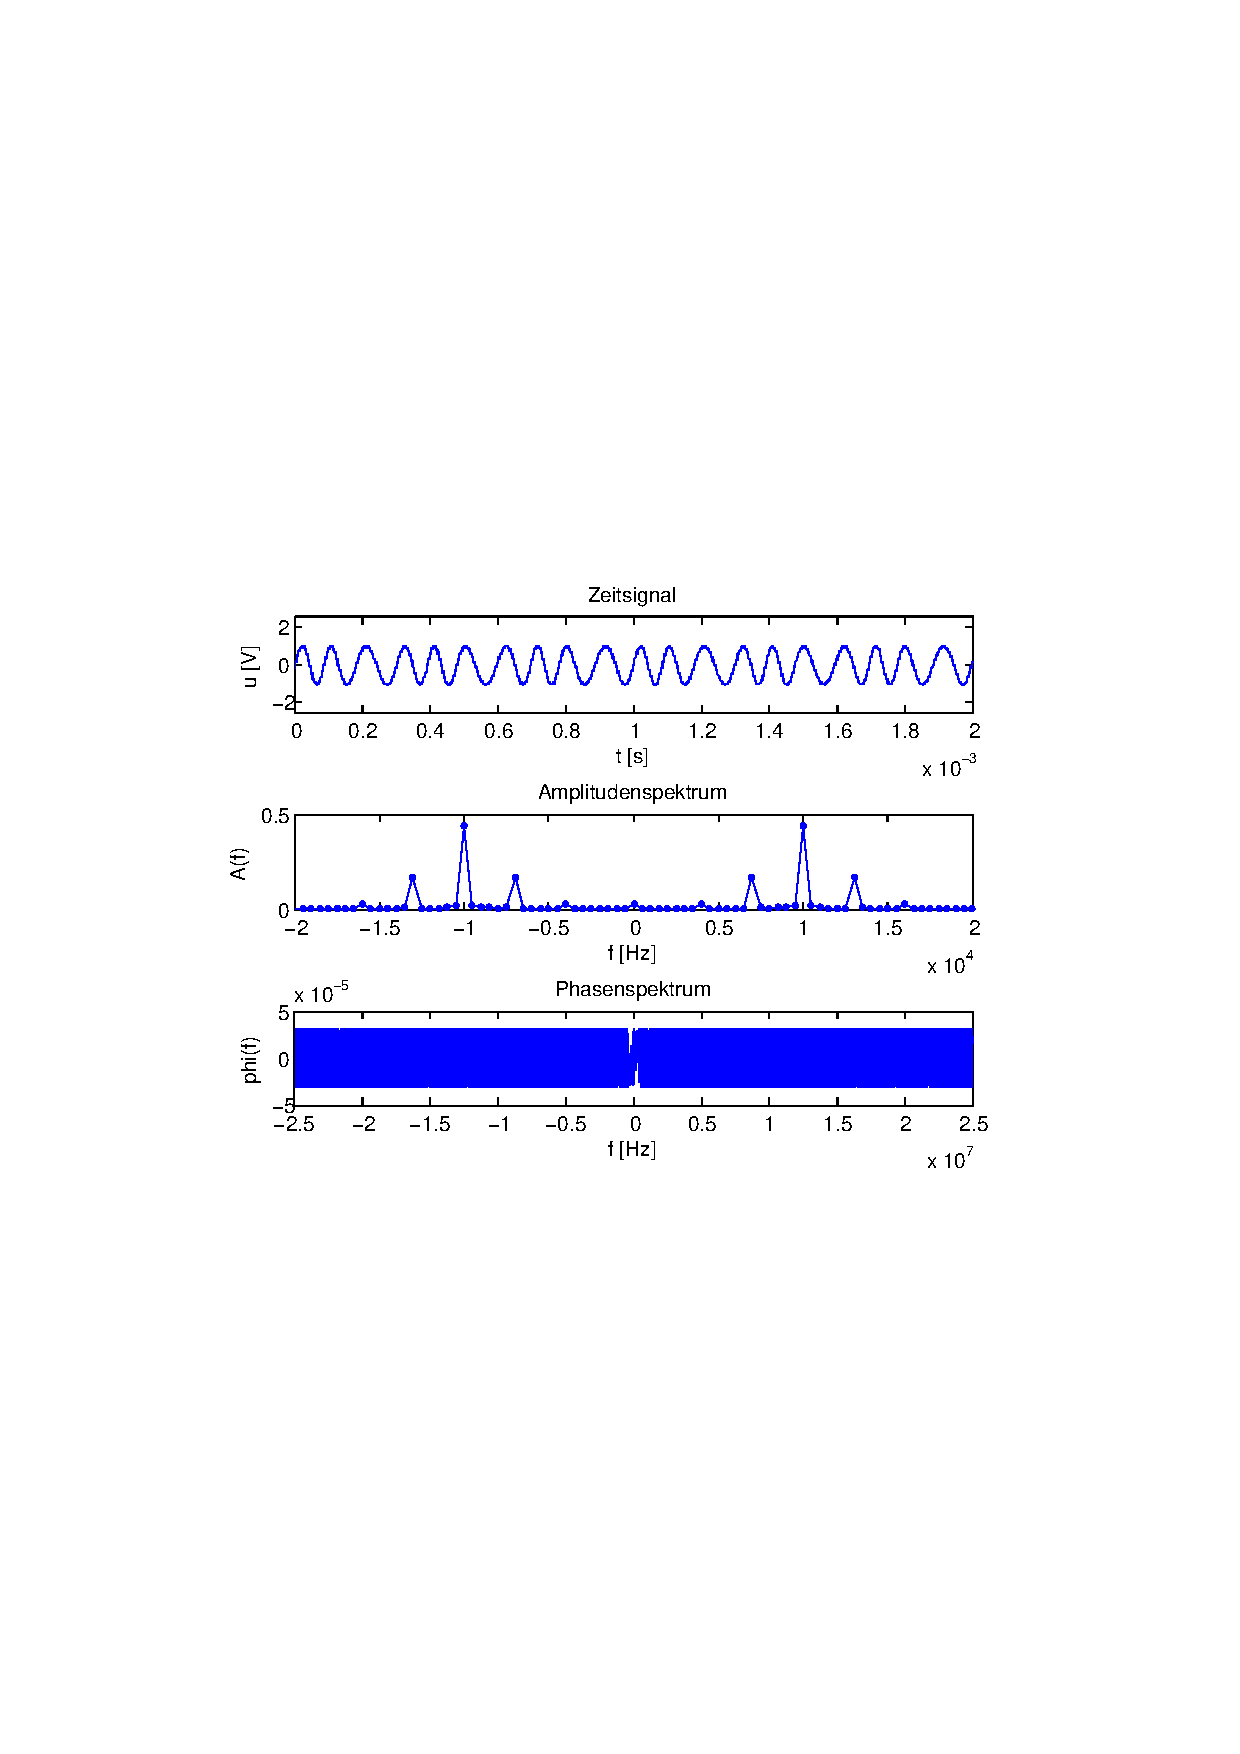
\includegraphics[scale=0.5, trim = 2cm 6.5cm 1.5cm
                        8.5cm, clip]{./Bilder/spektrum_sin3kHz}
                        %FIXME [width=640px, height=474px]
                        \caption{Spektrum für das Nutzsignal (3kHz, 1V)}
                    \end{figure}

                \end{minipage}
                \begin{minipage}{0.6\textwidth}

                     \begin{figure}[H]
                        \label{fig:}
                        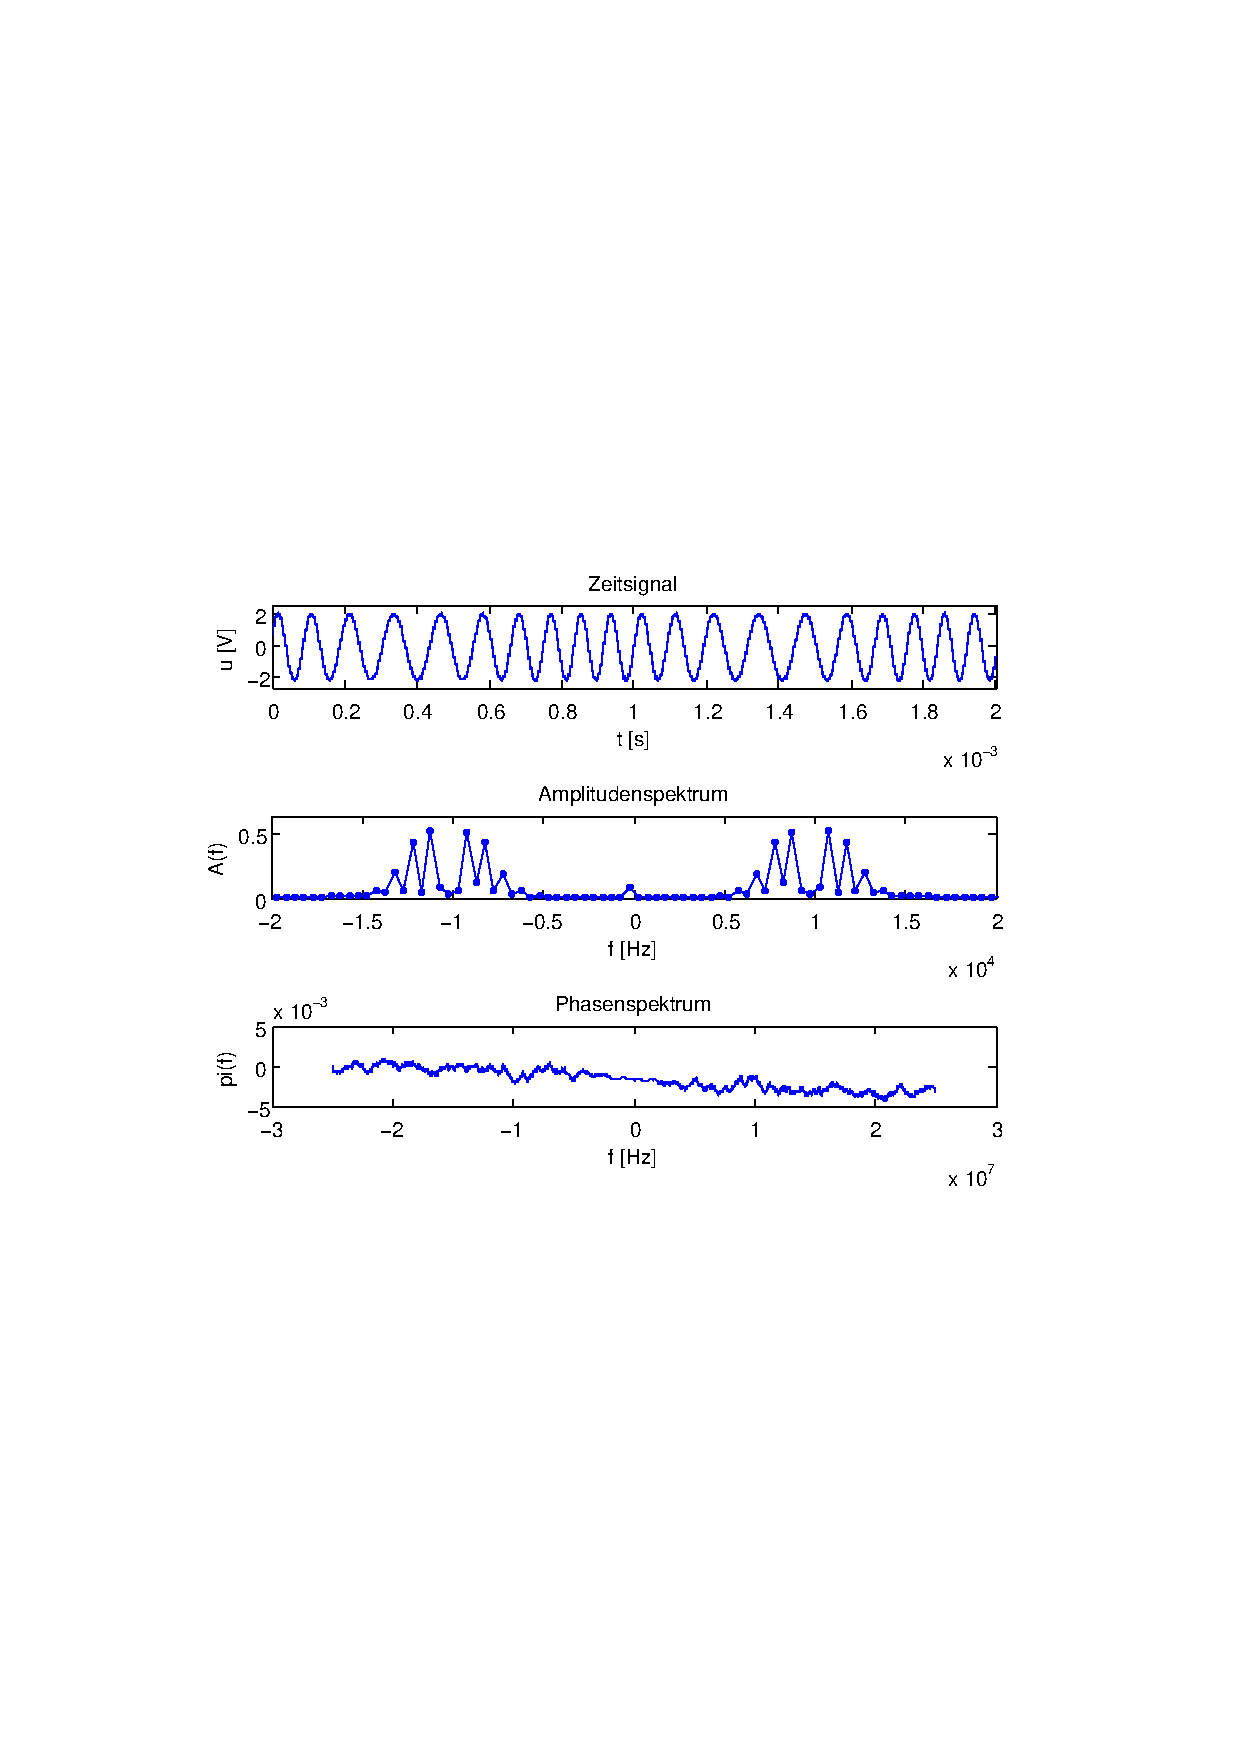
\includegraphics[scale=0.5, trim = 2cm 6.5cm 1.5cm
                        8.5cm, clip]{./Bilder/spektrum_sin1kHz}
                        %FIXME [width=640px, height=474px]
                        \caption{Spektrum für das Nutzsignal (1kHz, 1V)}
                    \end{figure}
               \vspace{-1.5em}

                \end{minipage}

            \end{tabular}
            \end{center}
        
        An den Spektren kann man sehen\ldots
        
        Um die Auswirkung von Frequenz und Amplitude genauer untersuchen zu
        können, führten wir noch weitere Sinusnutzsignal-Messungen durch mit den
        jeweiligen Amplituden $0.5V, 1V$ und $2V$, sowie den Frequenzen $50Hz,
        100Hz$ und $200Hz$. Folgende Spektren sind daraus entstanden:
        
               \begin{center}
            \begin{tabular}{ll}

            \hspace{-14em}
                \begin{minipage}{0.6\textwidth}

                    \begin{figure}[H]
                        \label{fig:}
                        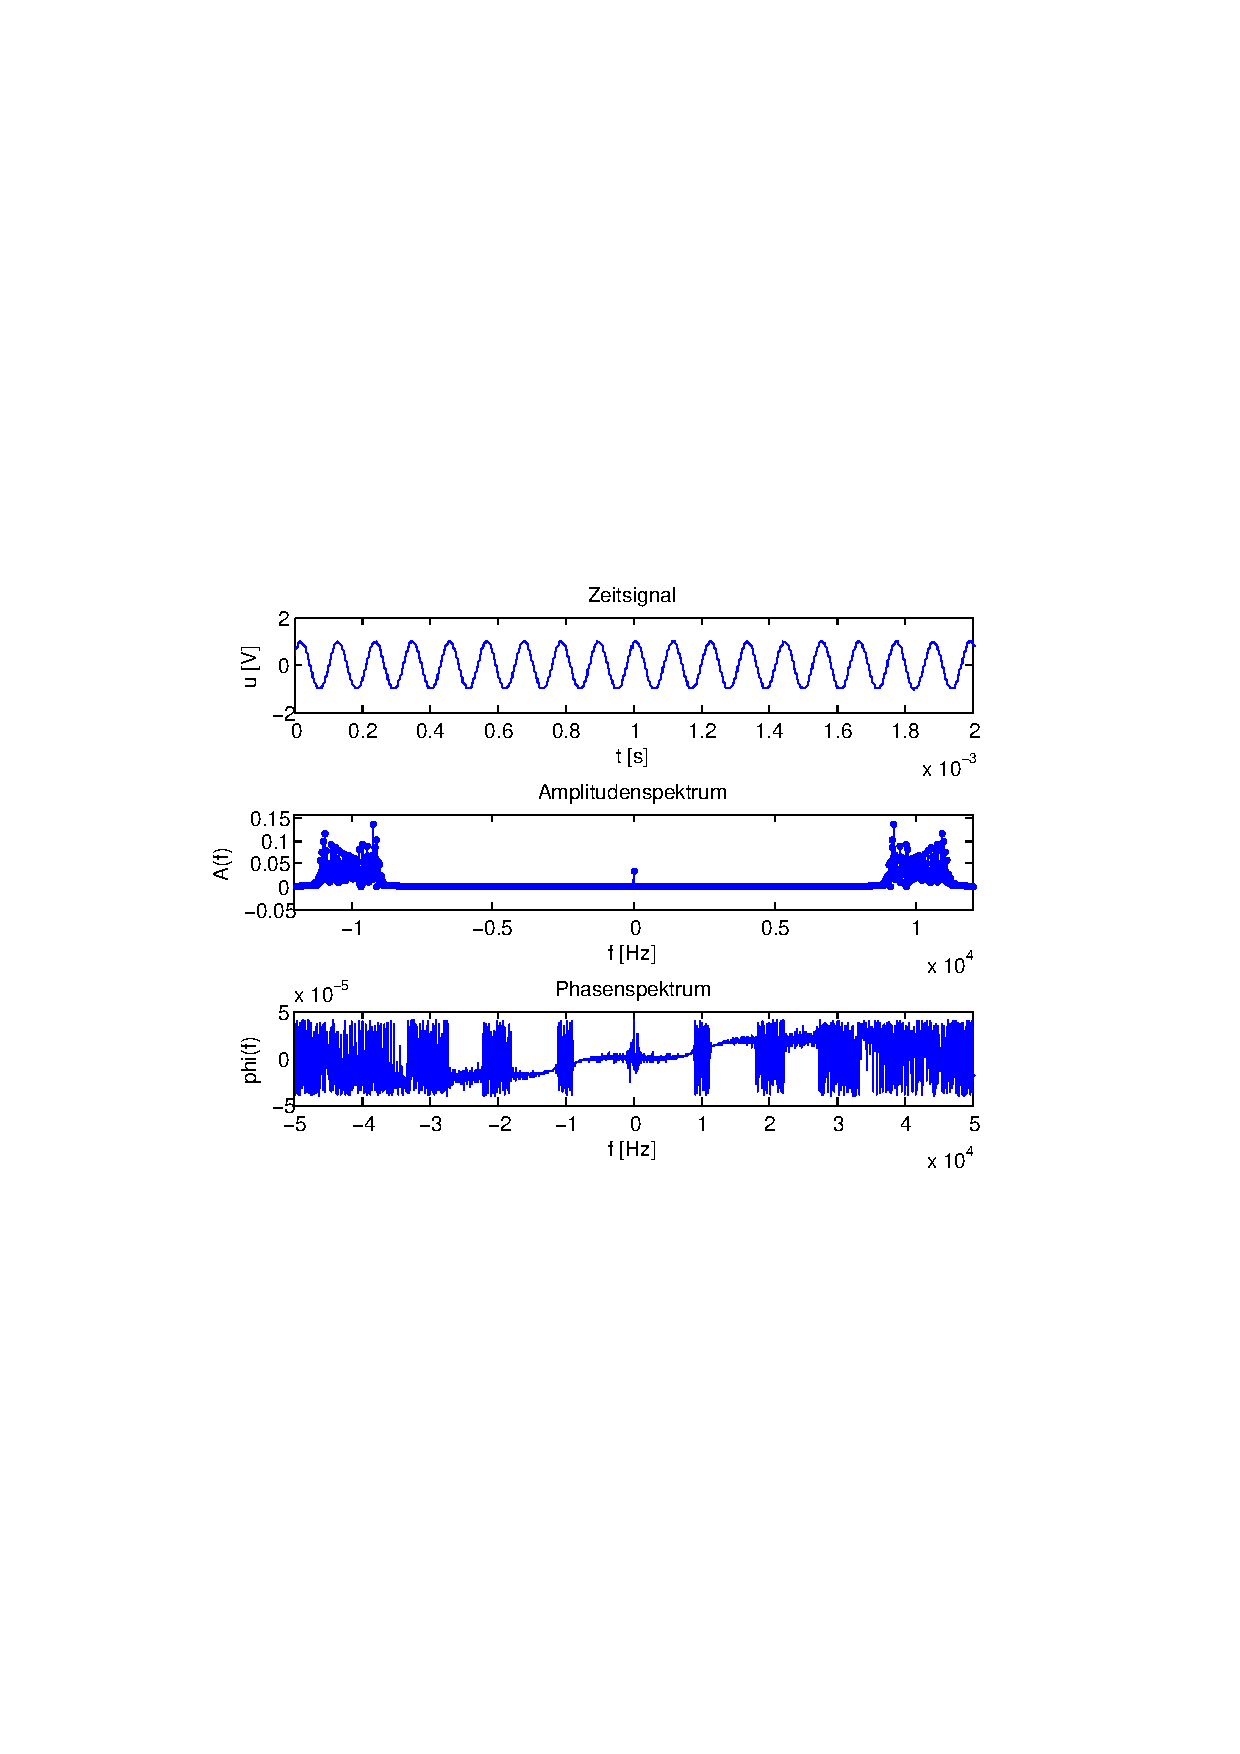
\includegraphics[scale=0.5, trim = 2cm 6.5cm 1.5cm
                        8.5cm, clip]{./Bilder/sin_a05_f50}
                        %FIXME [width=640px, height=474px]
                        \caption{Spektrum für Sinusnutzsignal (0.5V, 50Hz)}
                    \end{figure}

                \end{minipage}
                \begin{minipage}{0.6\textwidth}

                     \begin{figure}[H]
                        \label{fig:}
                        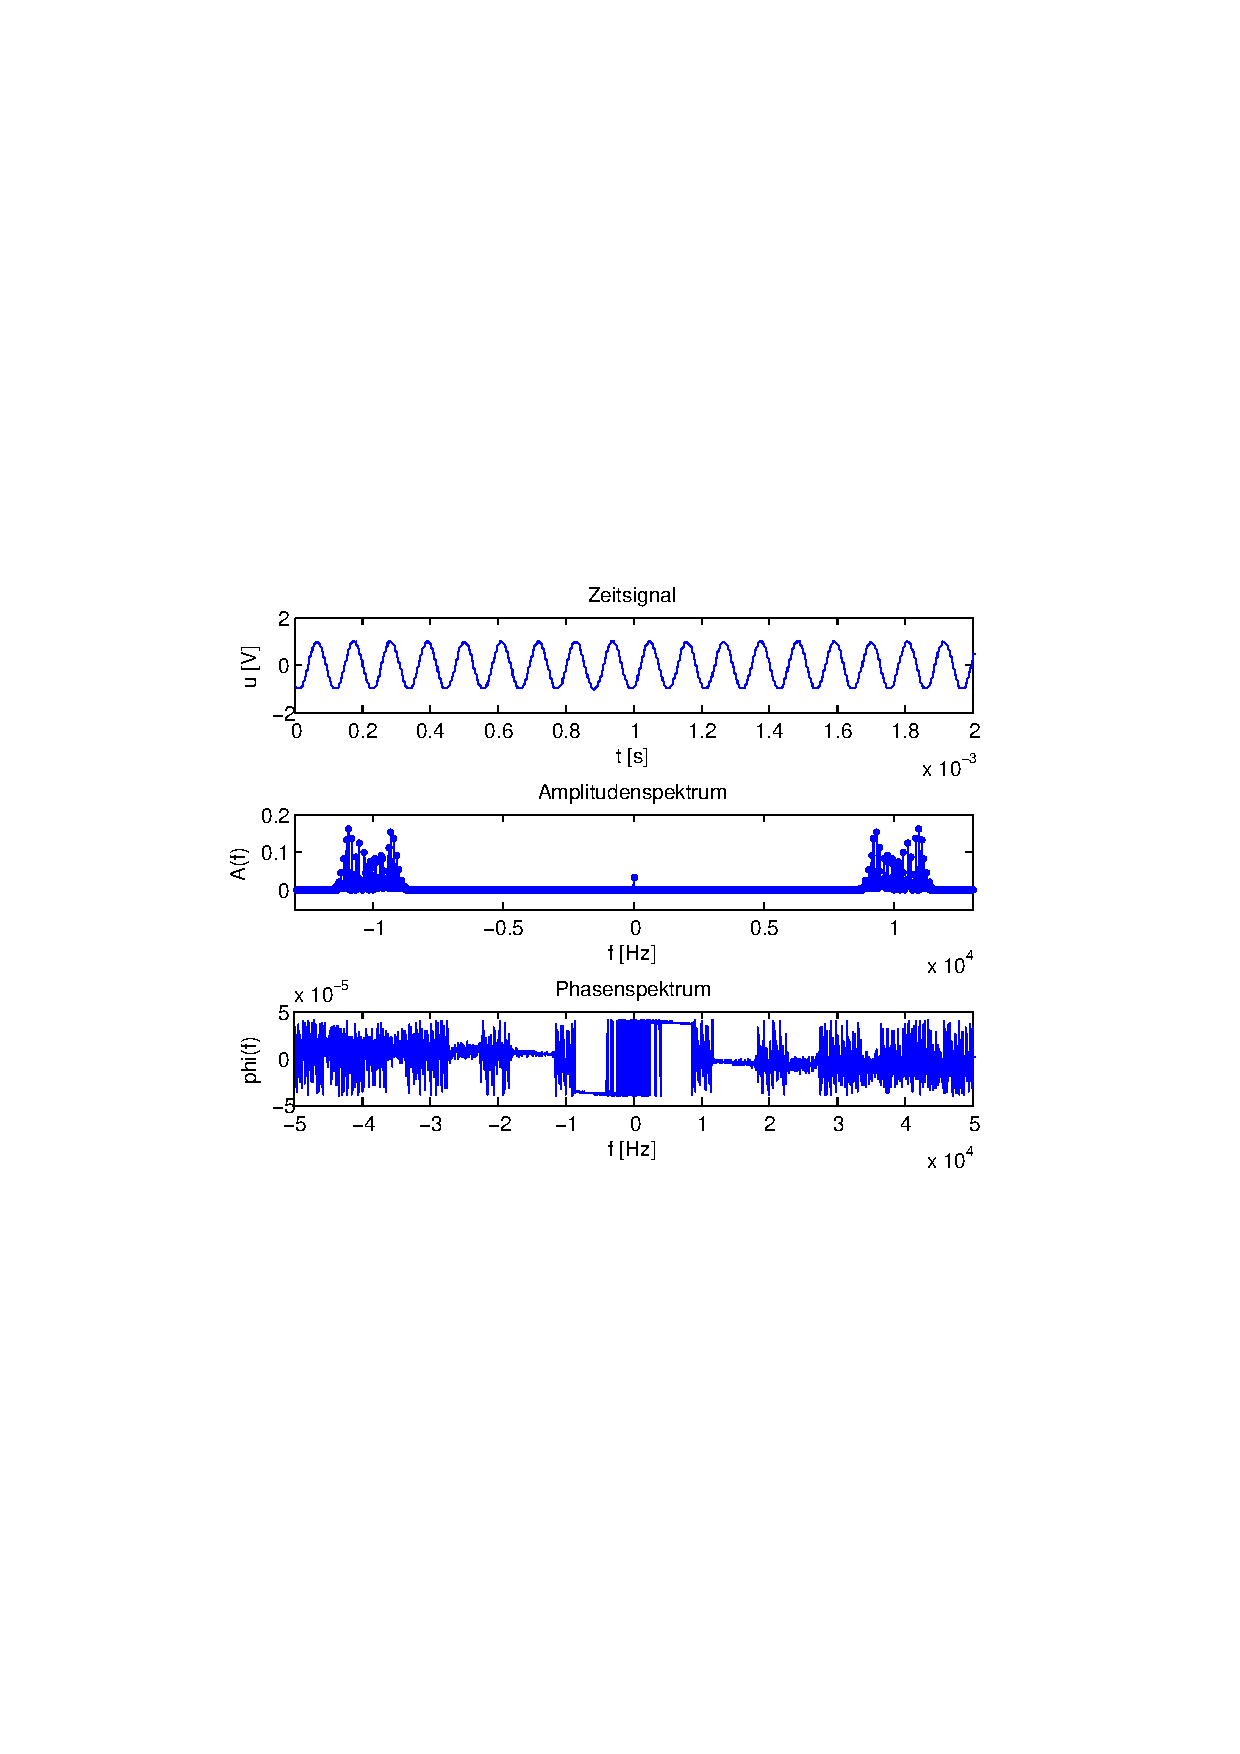
\includegraphics[scale=0.5, trim = 2cm 6.5cm 1.5cm
                        8.5cm, clip]{./Bilder/sin_a05_f100}
                        %FIXME [width=640px, height=474px]
                        \caption{Spektrum für Sinusnutzsignal (0.5V, 100Hz)}
                    \end{figure}
               \vspace{-1.5em}

                \end{minipage}

            \end{tabular}
            \end{center}
            
            %Erste Reihe mit 2 Bildern
            
                   \begin{center}
            \begin{tabular}{ll}

            \hspace{-14em}
                \begin{minipage}{0.6\textwidth}

                    \begin{figure}[H]
                        \label{fig:}
                        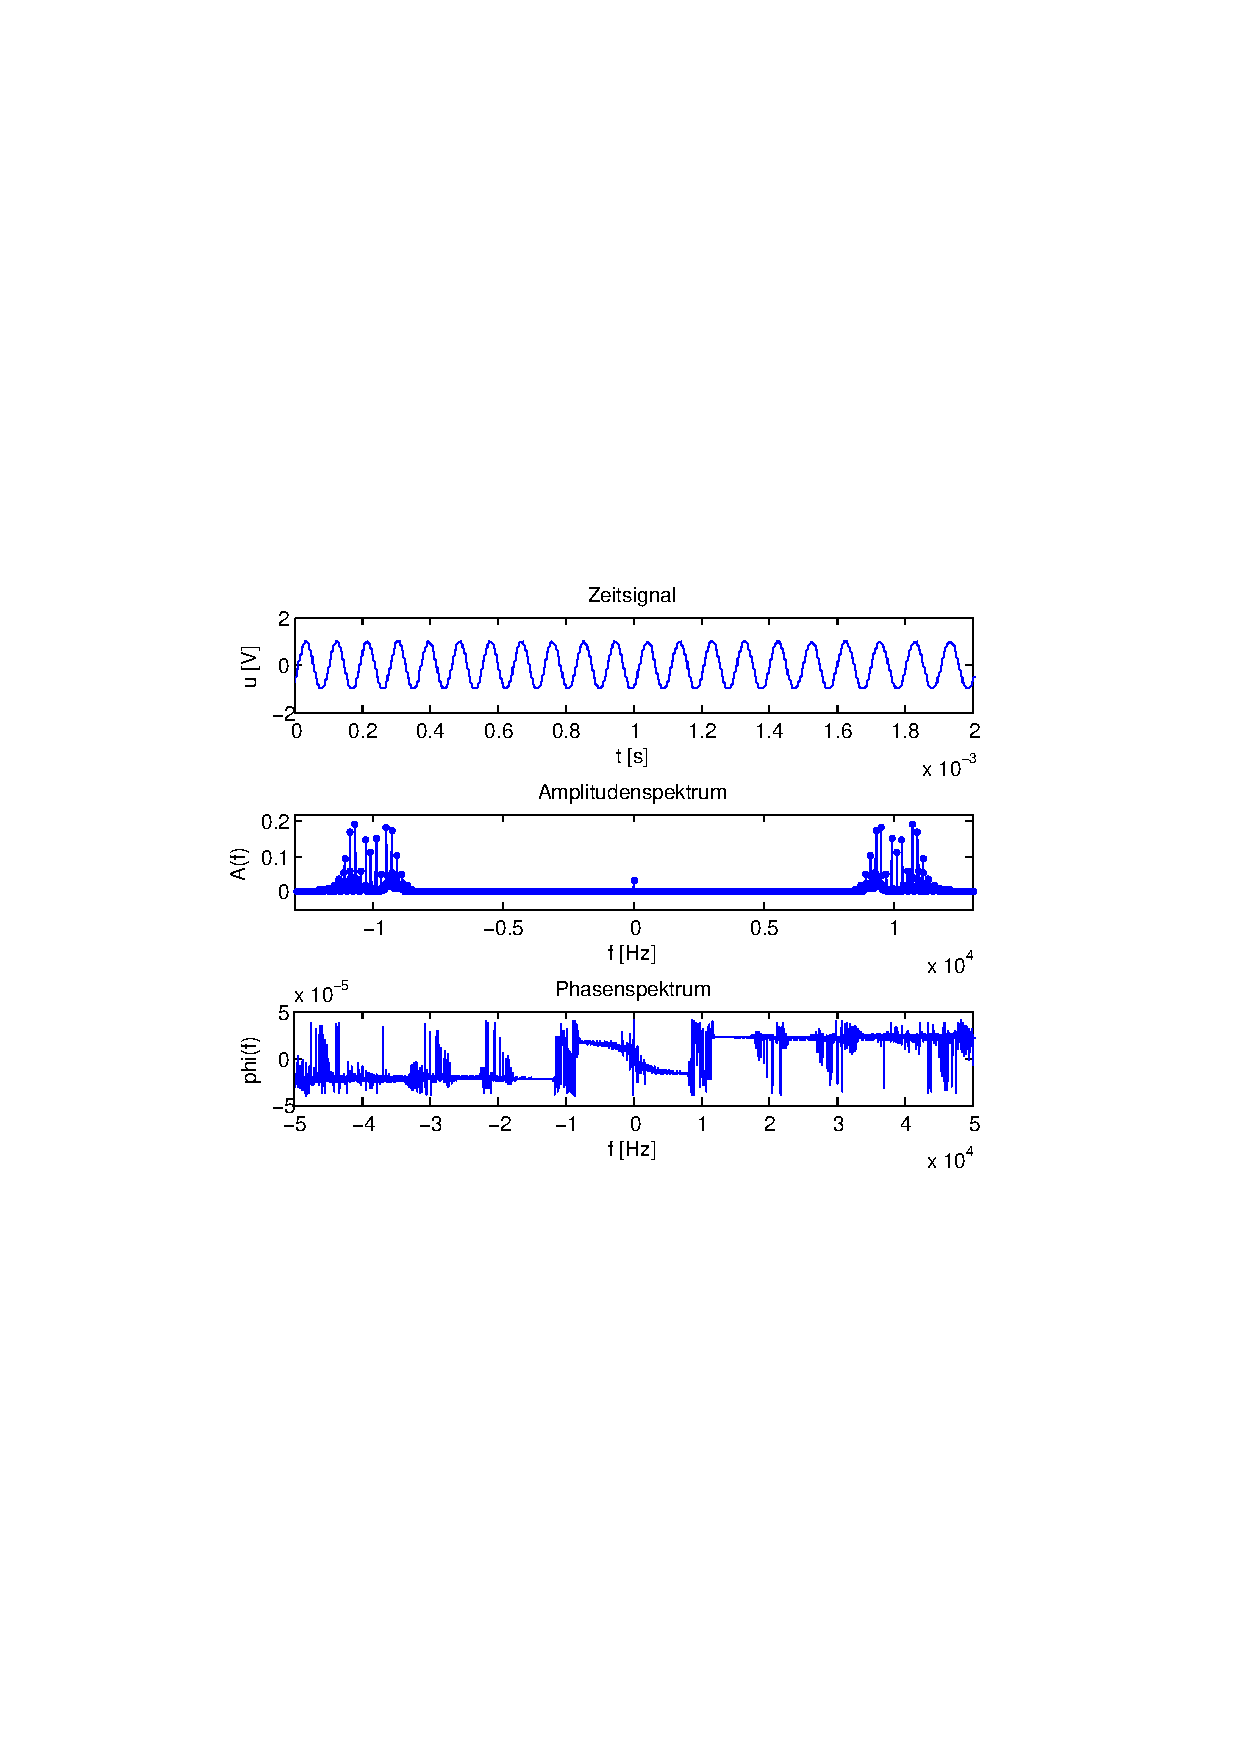
\includegraphics[scale=0.5, trim = 2cm 6.5cm 1.5cm
                        8.5cm, clip]{./Bilder/sin_a05_f200}
                        %FIXME [width=640px, height=474px]
                        \caption{Spektrum für moduliertes Sinusnutzsignal (0.5V,
                        200Hz)}
                    \end{figure}

                \end{minipage}
                \begin{minipage}{0.6\textwidth}

                     \begin{figure}[H]
                        \label{fig:}
                        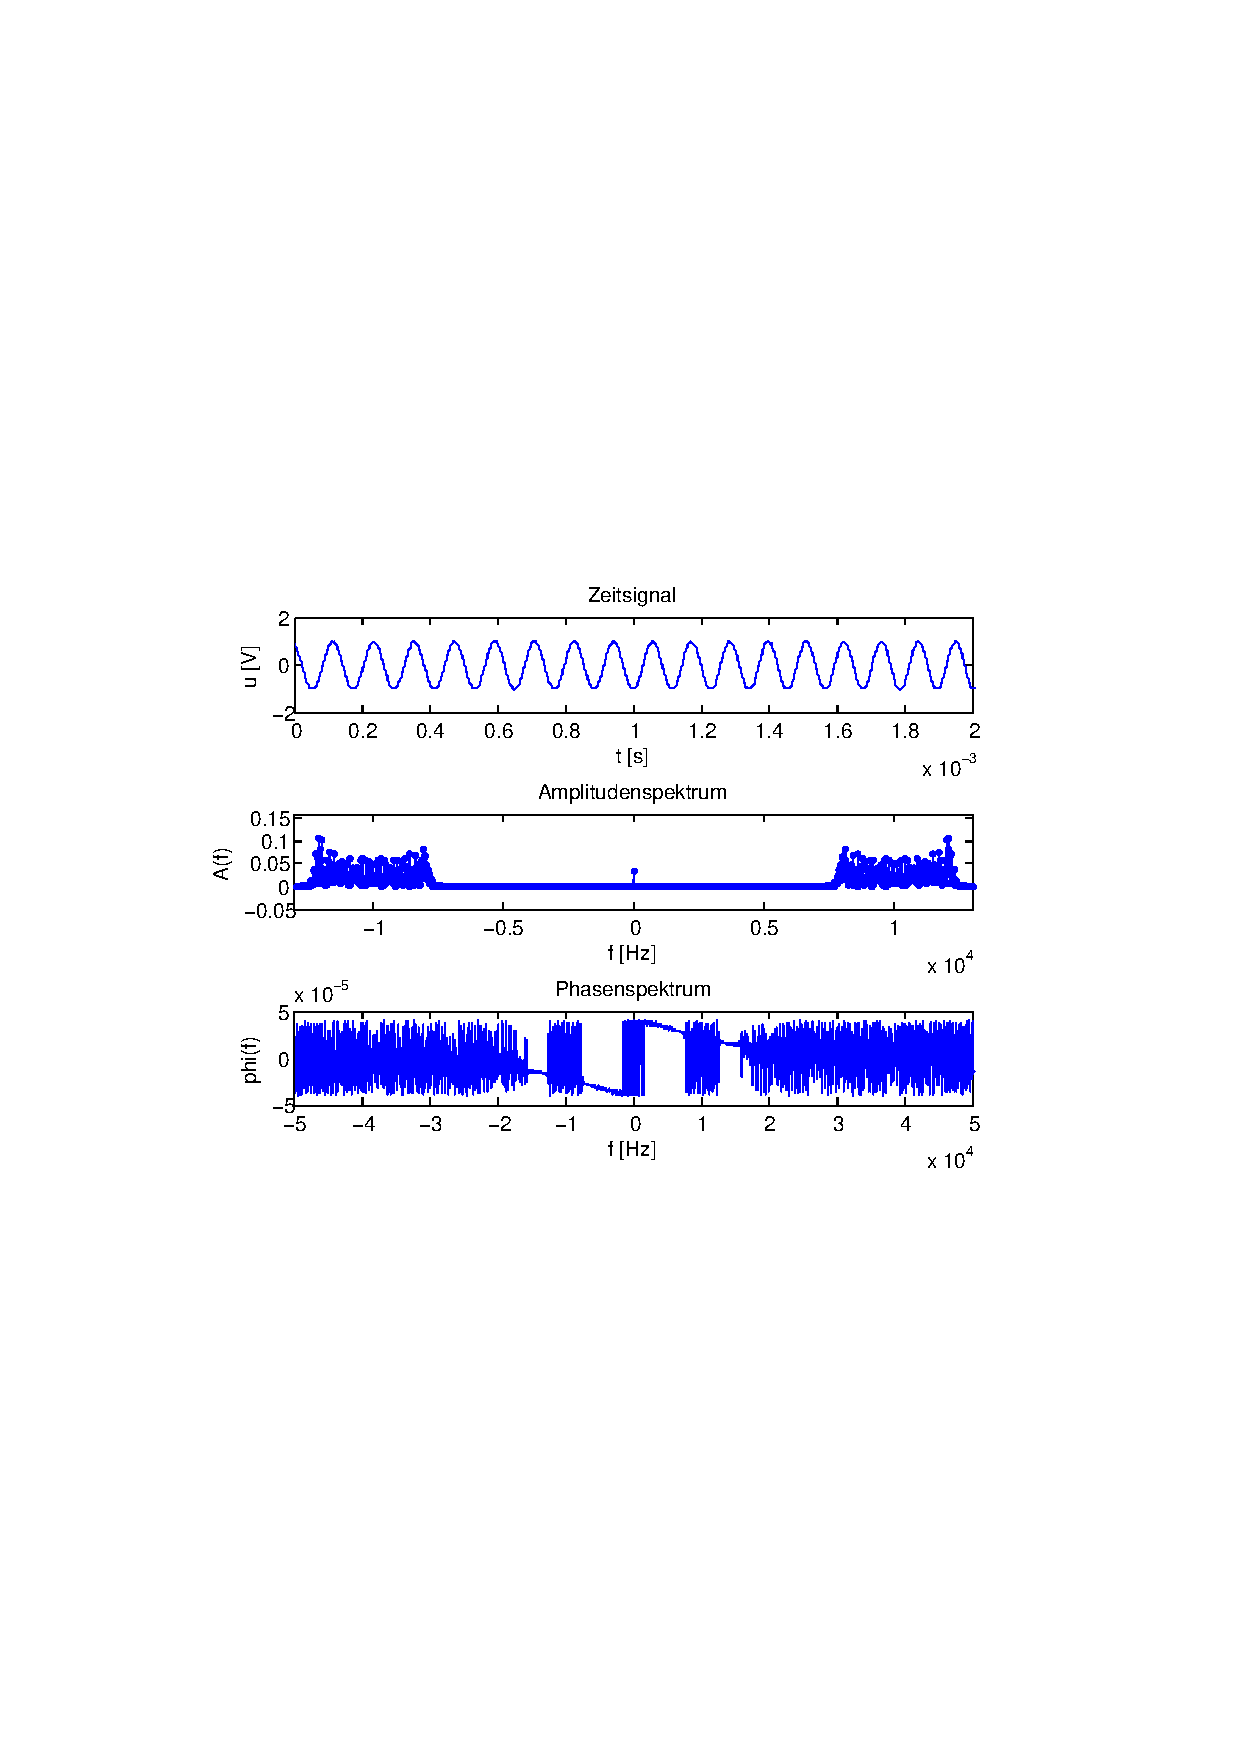
\includegraphics[scale=0.5, trim = 2cm 6.5cm 1.5cm
                        8.5cm, clip]{./Bilder/sin_a1_f50}
                        %FIXME [width=640px, height=474px]
                        \caption{Spektrum für moduliertes Sinusnutzsignal (1V,
                        50Hz)}
                    \end{figure}
               \vspace{-1.5em}

                \end{minipage}

            \end{tabular}
            \end{center}
        	
        	%Zweite Reihe mit 2 Bildern
        	   
        	       \begin{center}
            \begin{tabular}{ll}

            \hspace{-14em}
                \begin{minipage}{0.6\textwidth}

                    \begin{figure}[H]
                        \label{fig:}
                        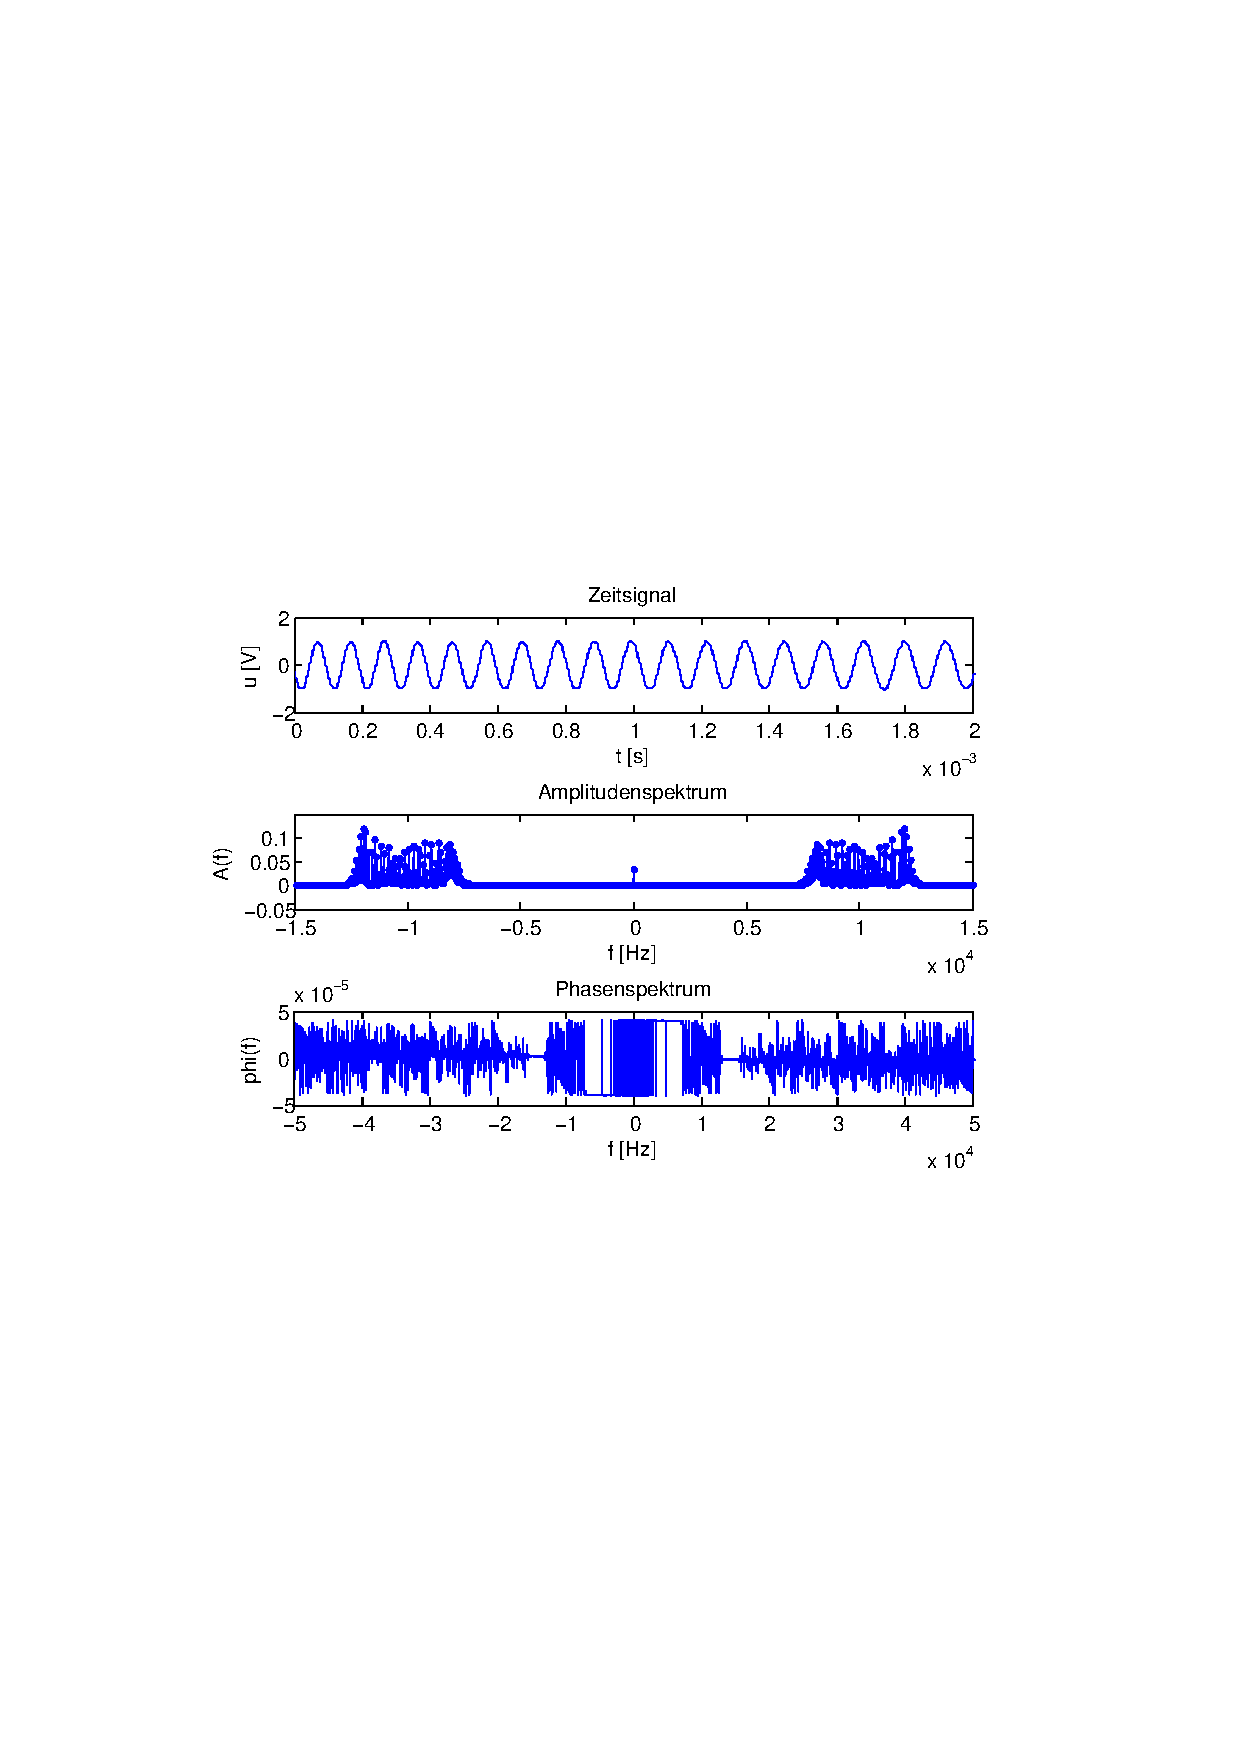
\includegraphics[scale=0.5, trim = 2cm 6.5cm 1.5cm
                        8.5cm, clip]{./Bilder/sin_a1_f100}
                        %FIXME [width=640px, height=474px]
                        \caption{Spektrum für moduliertes Sinusnutzsignal (1V,
                        100Hz)}
                    \end{figure}

                \end{minipage}
                \begin{minipage}{0.6\textwidth}

                     \begin{figure}[H]
                        \label{fig:}
                        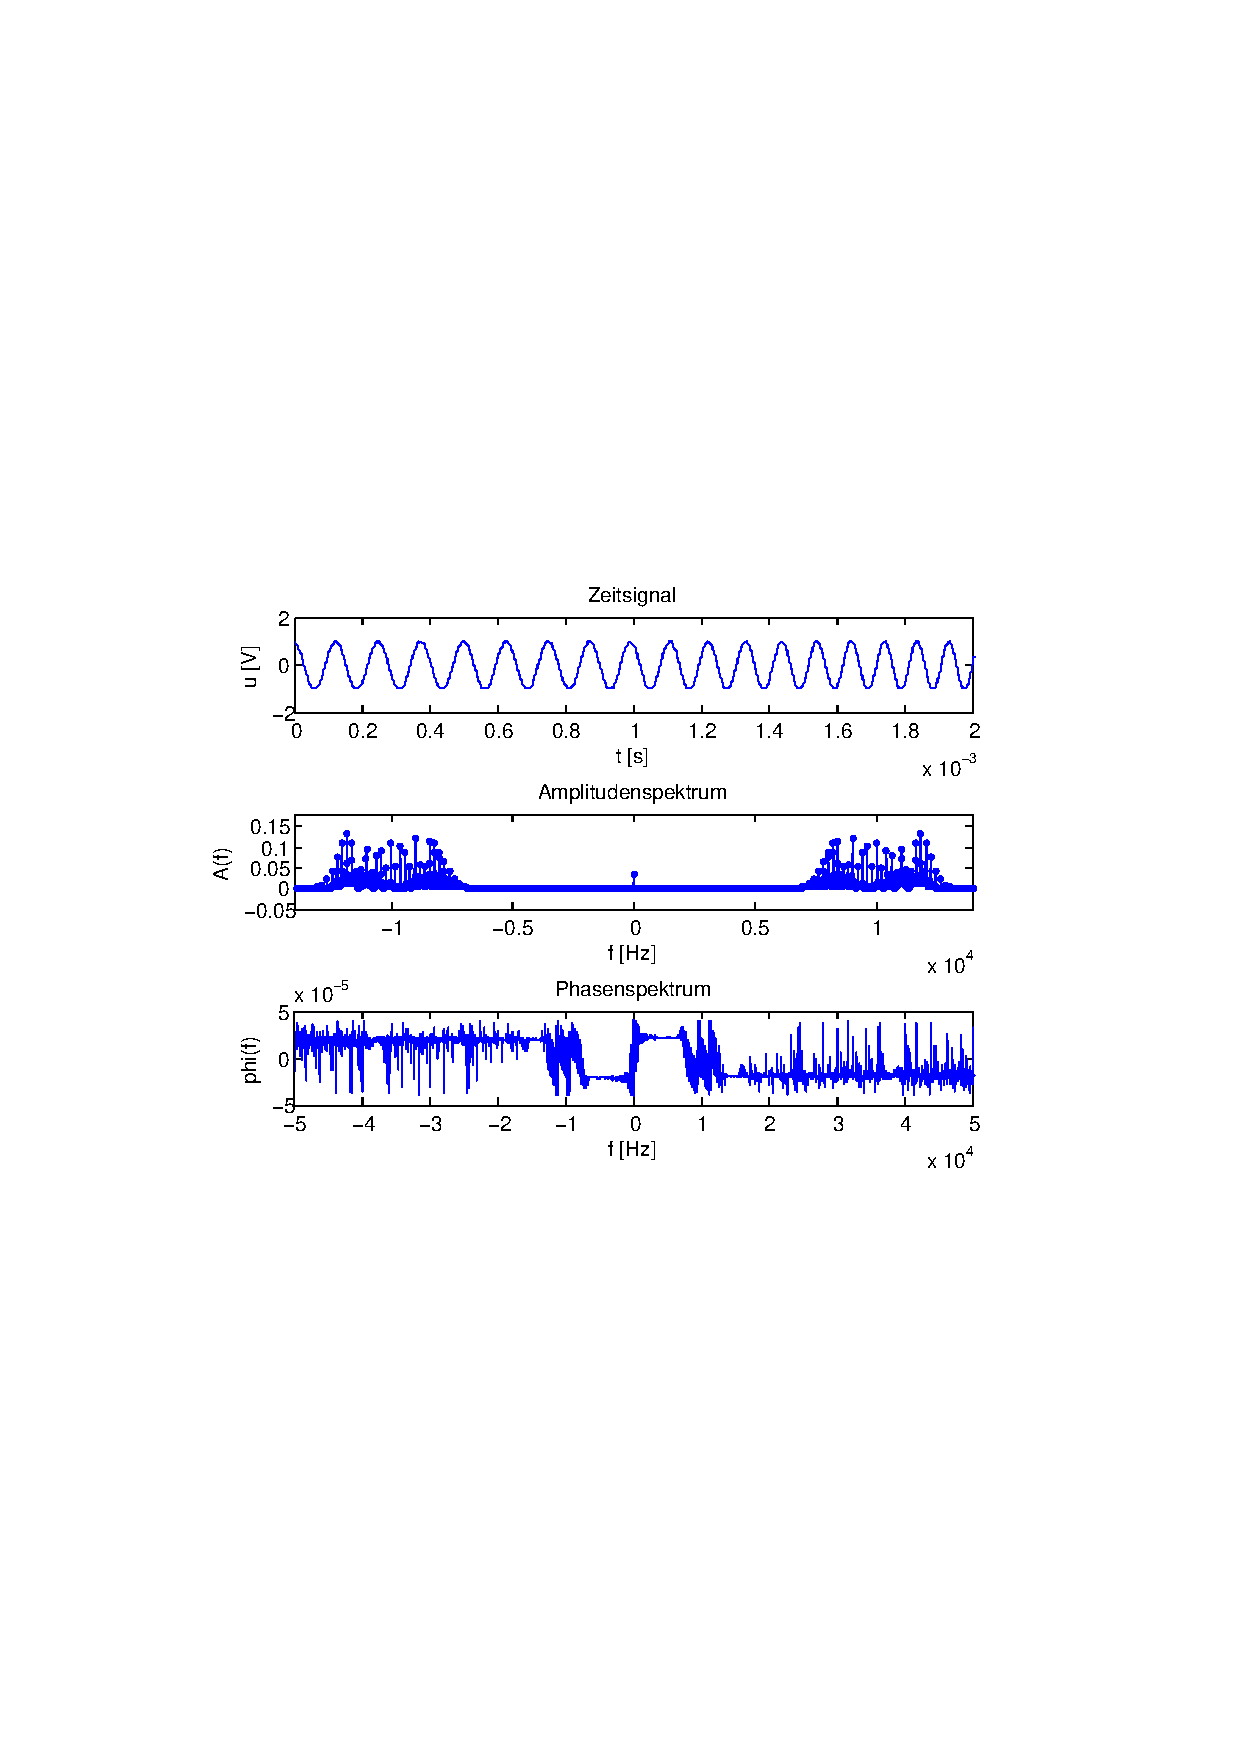
\includegraphics[scale=0.5, trim = 2cm 6.5cm 1.5cm
                        8.5cm, clip]{./Bilder/sin_a1_f200}
                        %FIXME [width=640px, height=474px]
                        \caption{Spektrum für moduliertes Sinusnutzsignal (1V,
                        200Hz)}
                    \end{figure}
               \vspace{-1.5em}

                \end{minipage}

            \end{tabular}
            \end{center}
        
        %Dreitte Reihe mit 2 Bildern
        
               \begin{center}
            \begin{tabular}{ll}

            \hspace{-14em}
                \begin{minipage}{0.6\textwidth}

                    \begin{figure}[H]
                        \label{fig:}
                        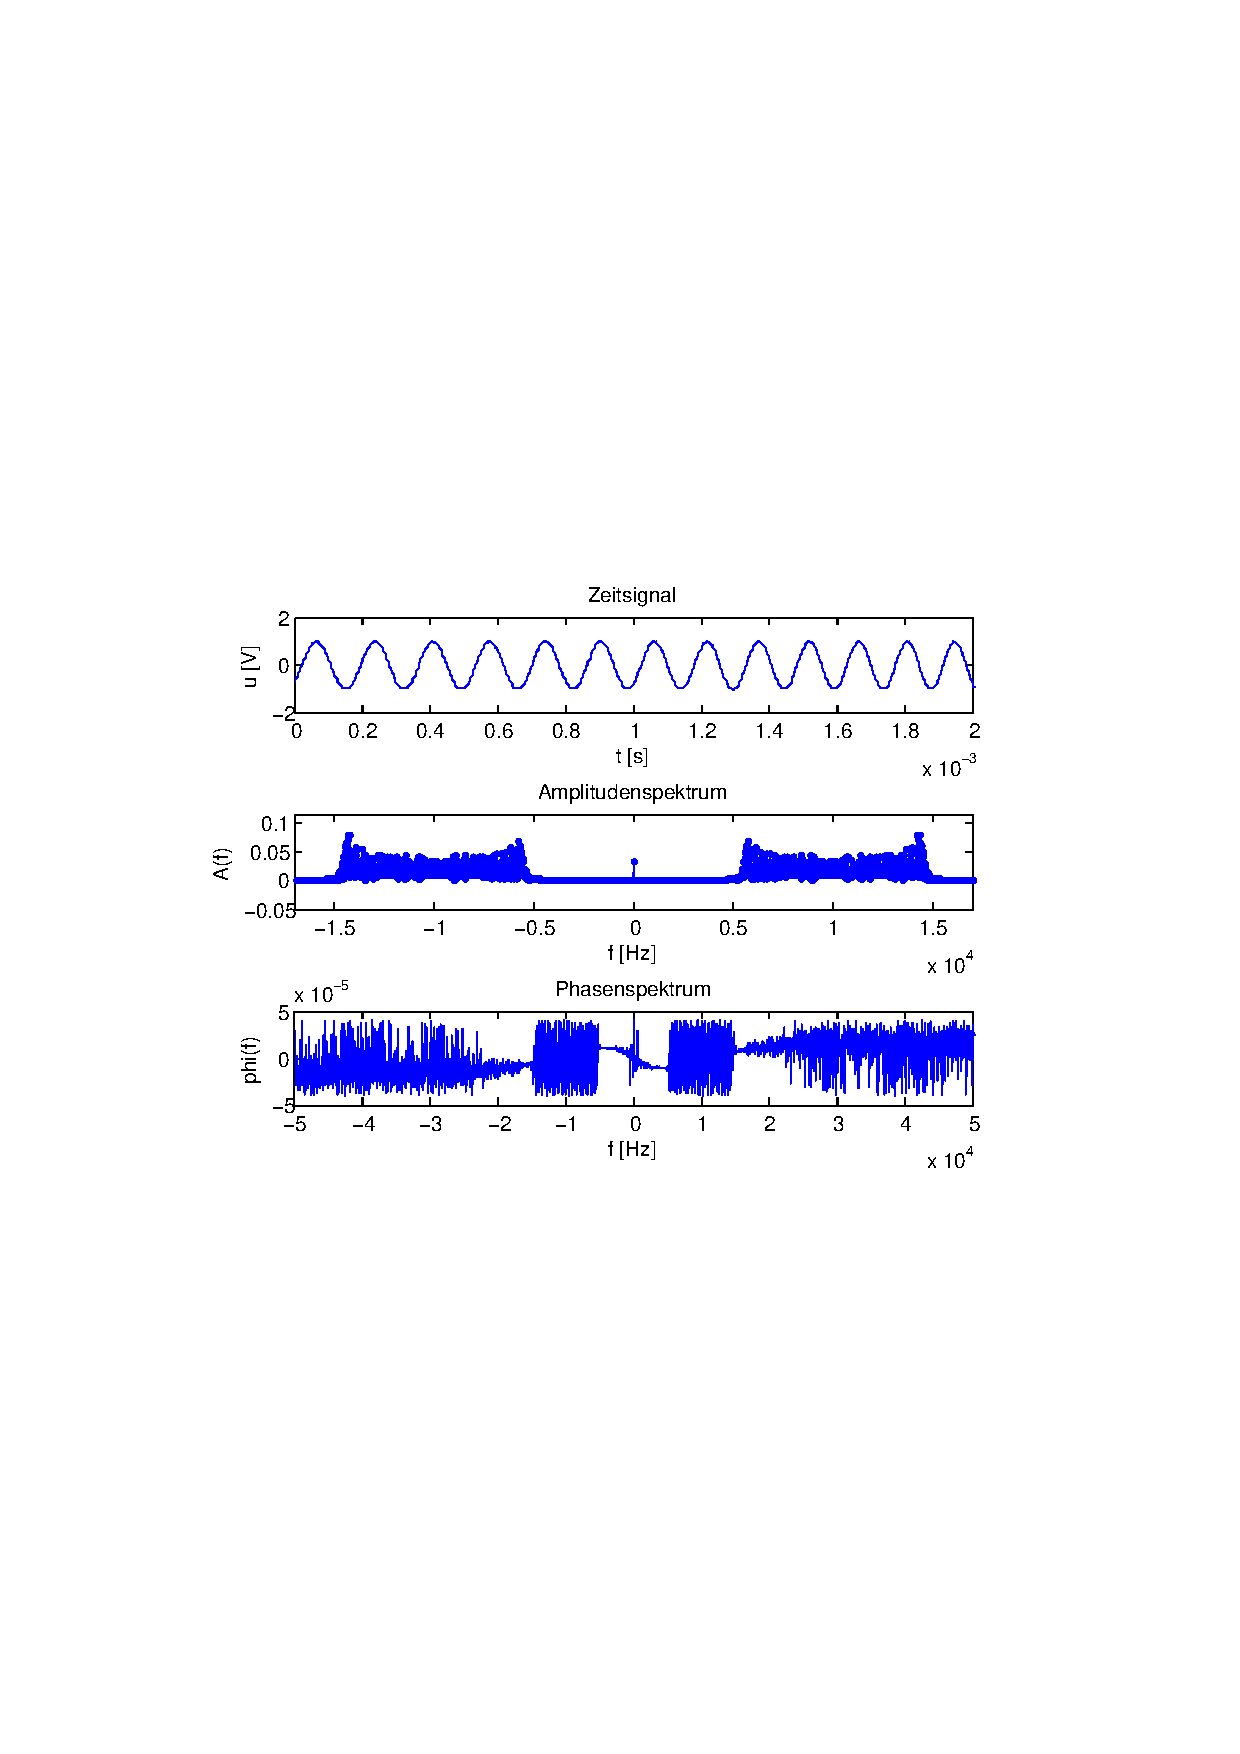
\includegraphics[scale=0.5, trim = 2cm 6.5cm 1.5cm
                        8.5cm, clip]{./Bilder/sin_a2_f50}
                        %FIXME [width=640px, height=474px]
                        \caption{Spektrum für moduliertes Sinusnutzsignal (2V,
                        50Hz)}
                    \end{figure}

                \end{minipage}
                \begin{minipage}{0.6\textwidth}

                     \begin{figure}[H]
                        \label{fig:}
                        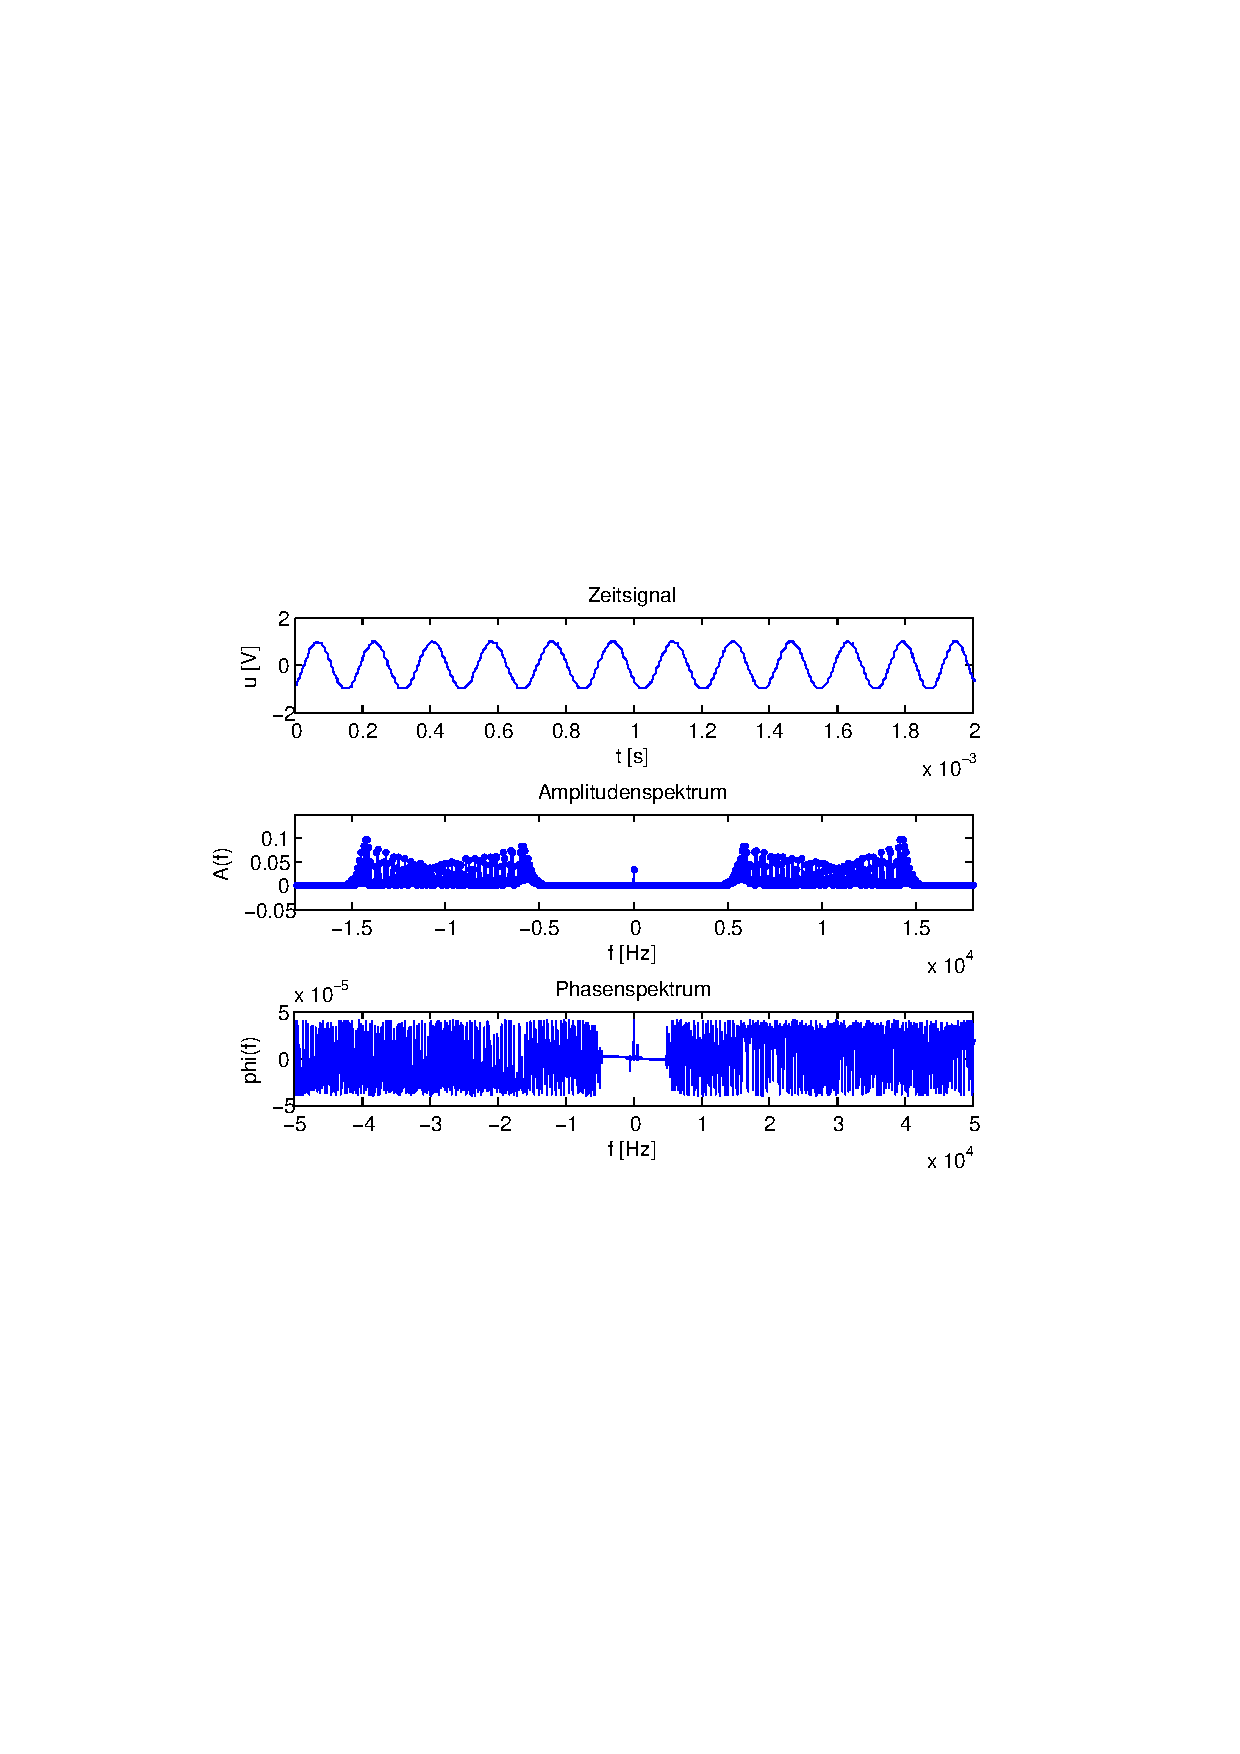
\includegraphics[scale=0.5, trim = 2cm 6.5cm 1.5cm
                        8.5cm, clip]{./Bilder/sin_a2_f100}
                        %FIXME [width=640px, height=474px]
                        \caption{Spektrum für moduliertes Sinusnutzsignal (2V,
                        100Hz)}
                    \end{figure}
               \vspace{-1.5em}

                \end{minipage}

            \end{tabular}
            \end{center}
            
            %Vierte Reihe mit nur einem Bild
            
             \begin{figure}[H] \centering
                    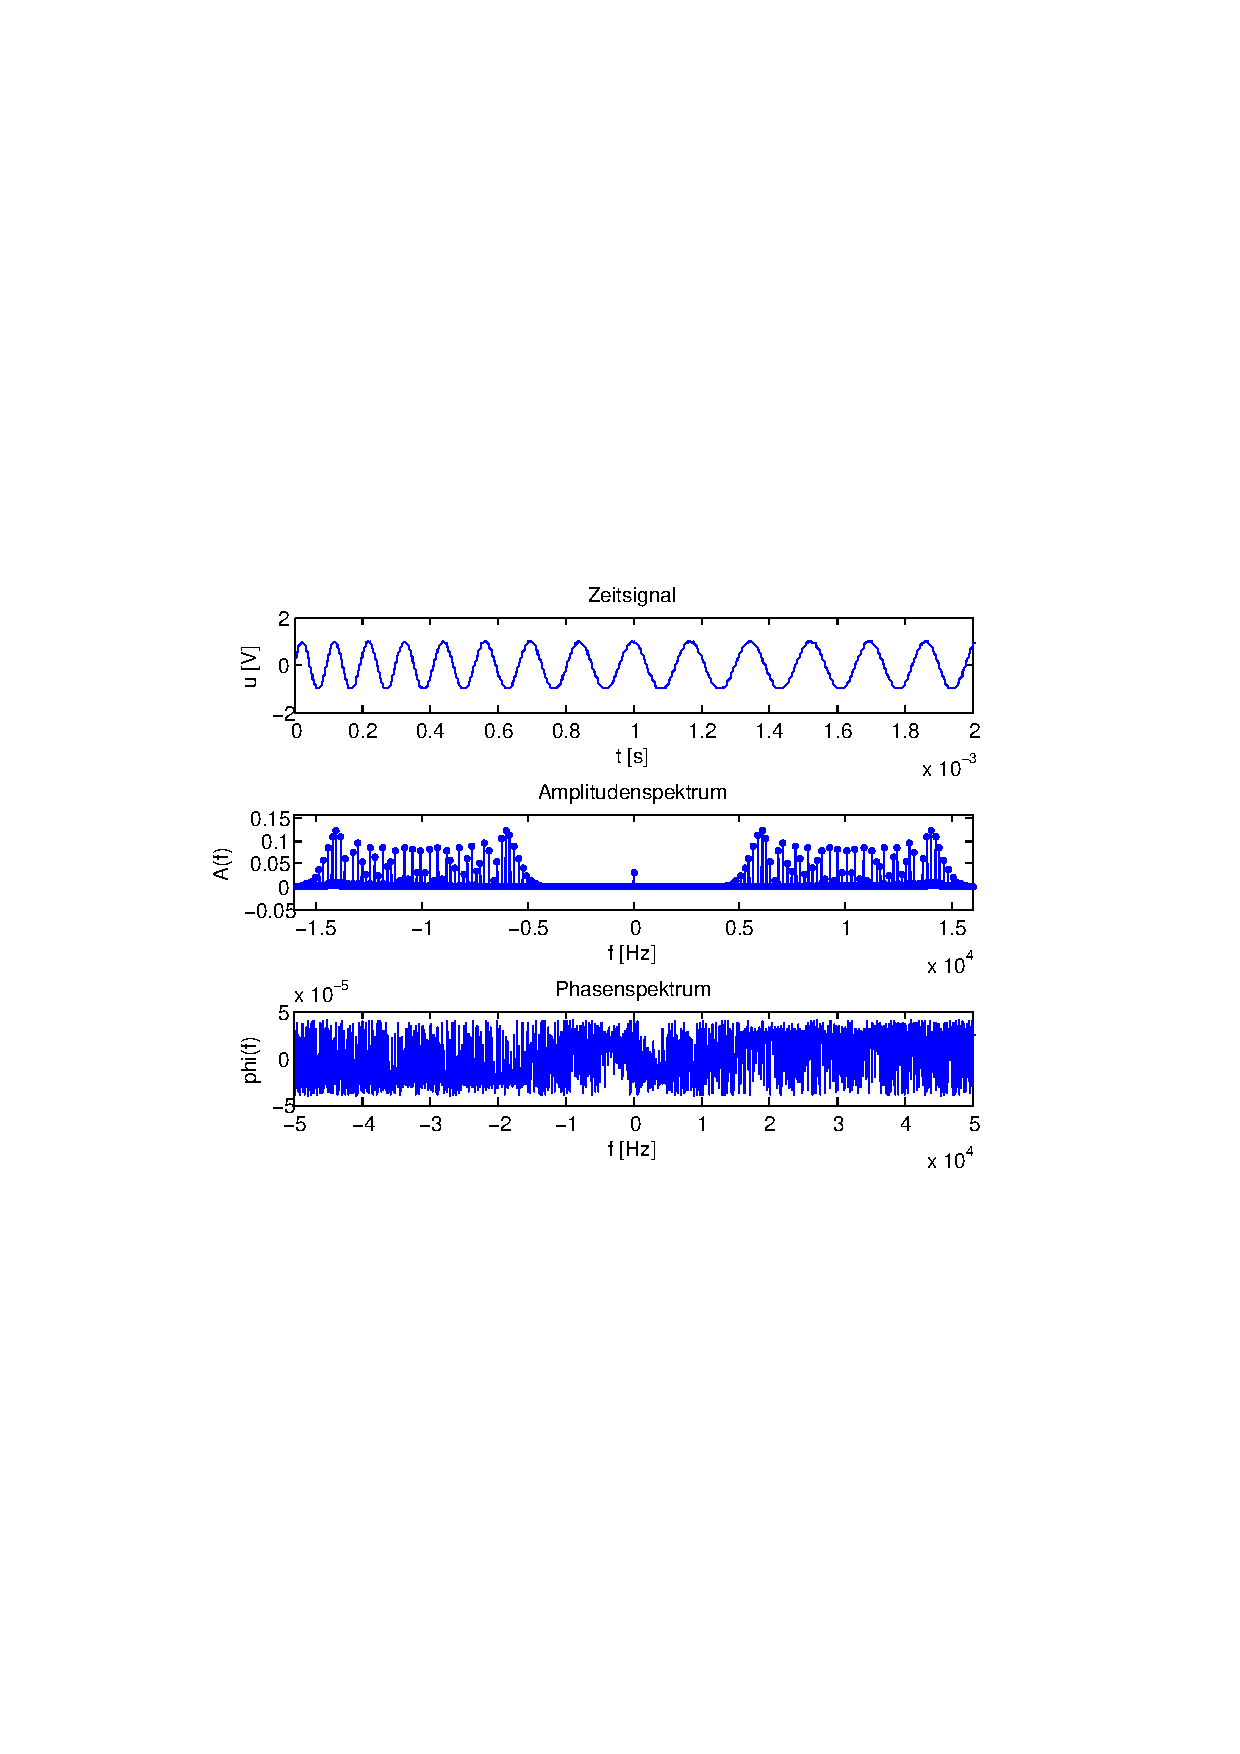
\includegraphics[scale=0.5, trim = 2cm 6.5cm 1.5cm 8.5cm,
                    clip]{./Bilder/sin_a2_f200}
                        \caption{Spektrum für moduliertes Sinusnutzsignal (2V,
                        200Hz)}
                \end{figure}
            
            
            An den Unterschiedlichen Spektren lässt sich eine Tendenz entdecken.
            Beispielsweise an den Spektren mit der Eingangssignalamplitude $0.5
            V$. Dabei öässt sich erkennen, dass die Amplitude der Impulse im
            Betragsspektrum höher mit wachsender Frequenz höher werden. An der
            Stelle in der Frequenzachse ändert sich dabei nichts. Die gleiche
            Beobachtung kann man auch mit der Messreihe der Nutzsignale mit der
            Amplitude $1V$ und $2V$ machen. Die wachsende Amplitude dagegen
            bewirkt, dass die auftretenden Impulsgruppen breiter werden und mehr
            Frequenzen benötigen. Somit kann man abschließend zusammenfassen,
            dass die steigende Amplitude des Nutzsignals im modulierten Spektrum
            zu einer höheren Amplitude und die wachsende Frequenz zu einem
            breiteren Freuquenzband führt.
            
            Bei der FM-Demodulation wurde das Comparator- und das Twin Pulse
            Generator-Modul eingesetzt. Die Funktion beider Module wurde bereits
            in der Durchführung ausreichend erläutert. Hier werden nun die
            Ausgänge der jeweiligen Module miteinander verglichen. Dabei gehen
            wir genauso vor, wie auch in der Durchführung.\\
            Als erstes wird bei fester Sendesignalfrequenz der Comparatorausgang
            betrachtet:
            
            
             \begin{figure}[H] \centering
                    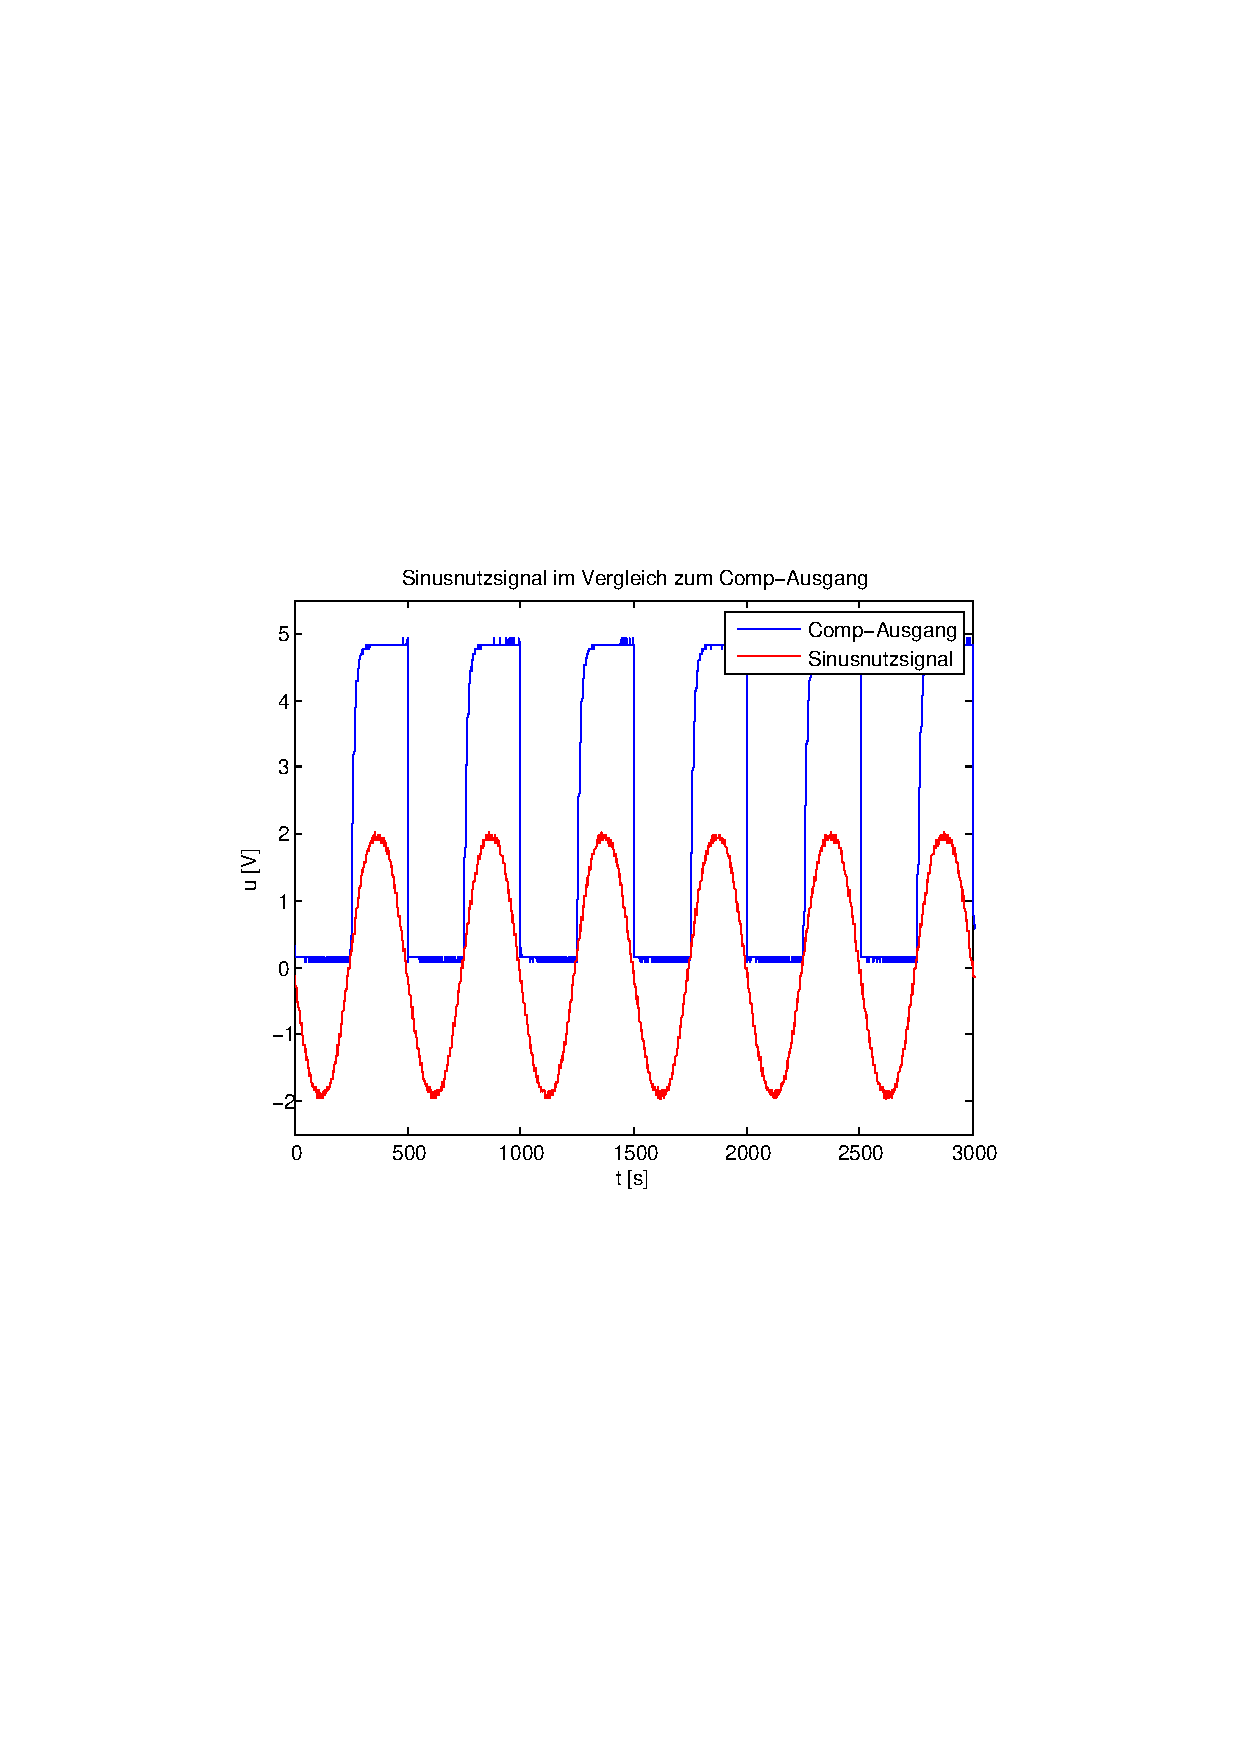
\includegraphics[scale=0.5, trim = 2cm 6.5cm 1.5cm 8.5cm,
                    clip]{./Bilder/sin_vs_comp}
                        \caption{Vergleich zwischen festem Sendesignal und
                        Signalverlauf am Comparator}
                \end{figure}
            
           Hier kann man sehr genau die Funktion des Comparator erkennen. Da wir
           einen Sinus ohne Offste verwenden und die verwendete Referenzspannung
           $0V$ beträgt, wird der Comp-Ausgang wie erwartet auf das high Signalm 
           gesetzt, sobald das Sendesignal vom negativen in den positiven
           Bereich übergeht. Im umgekehrten Fall wird der Comp-Ausgang auf low
           gesetzt. Somit entspricht diese Messung unseren Erwartungen.\\
           Als nächstes werden Sendesignal und TPG-Ausgang in den Vergleich
           gesetzt:
             
             \begin{figure}[H] \centering
                    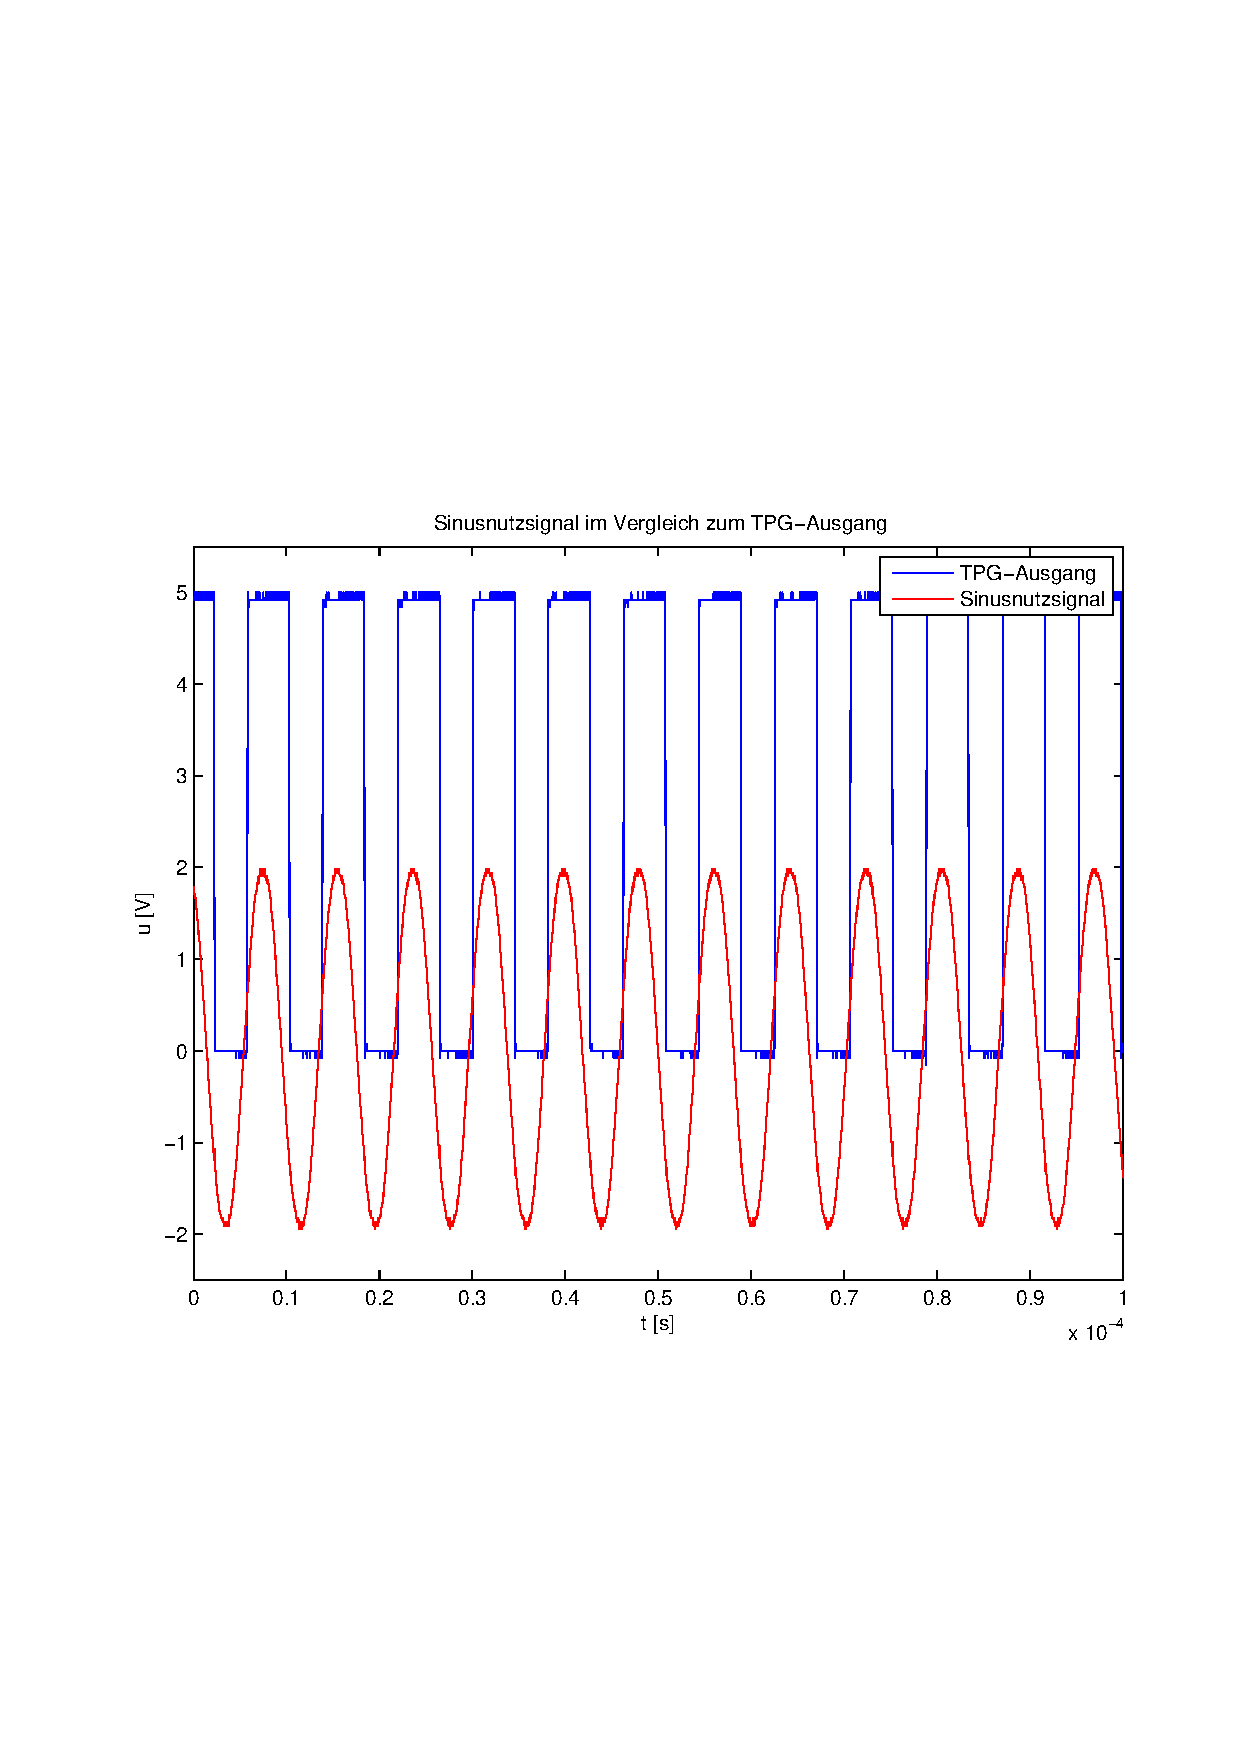
\includegraphics[scale=0.5, trim = 2cm 6.5cm 1.5cm 8.5cm,
                    clip]{./Bilder/sin_vs_tpg}
                        \caption{Vergleich zwischen festem Sendesignal und
                        Signalverlauf am TPG}
                \end{figure}
           
           An diesem Ergebnis können wir sehen, dass der TPG-Ausgang und der
           Comp-Ausgang fast das gleiche Signal liefern. Auch dies entspricht
           unseren Erwartungen, da der TPG bei jeder steigenden Flanke ein
           Rechteckimpuls ausgibt, also quasi aus einem Rechteck ein weiteres
           Rechteck macht. Ein kleiner Unterschied ist aber im Delay bemerkbar.
           Da der TPG erst nach dem Comparator vom Signal durchlaufen wird, ist
           dieses kleine Delay zwischen festem Sendesignal und dem
           TPG-Ausgangssignal nicht überraschend.\\
           
           Das der Comparator und der TPG fast das gleiche Signal ausgeben wird
           nochmal im Vergleich ihrer Ausgangssignale deutlich:
           
            
             \begin{figure}[H] \centering
                    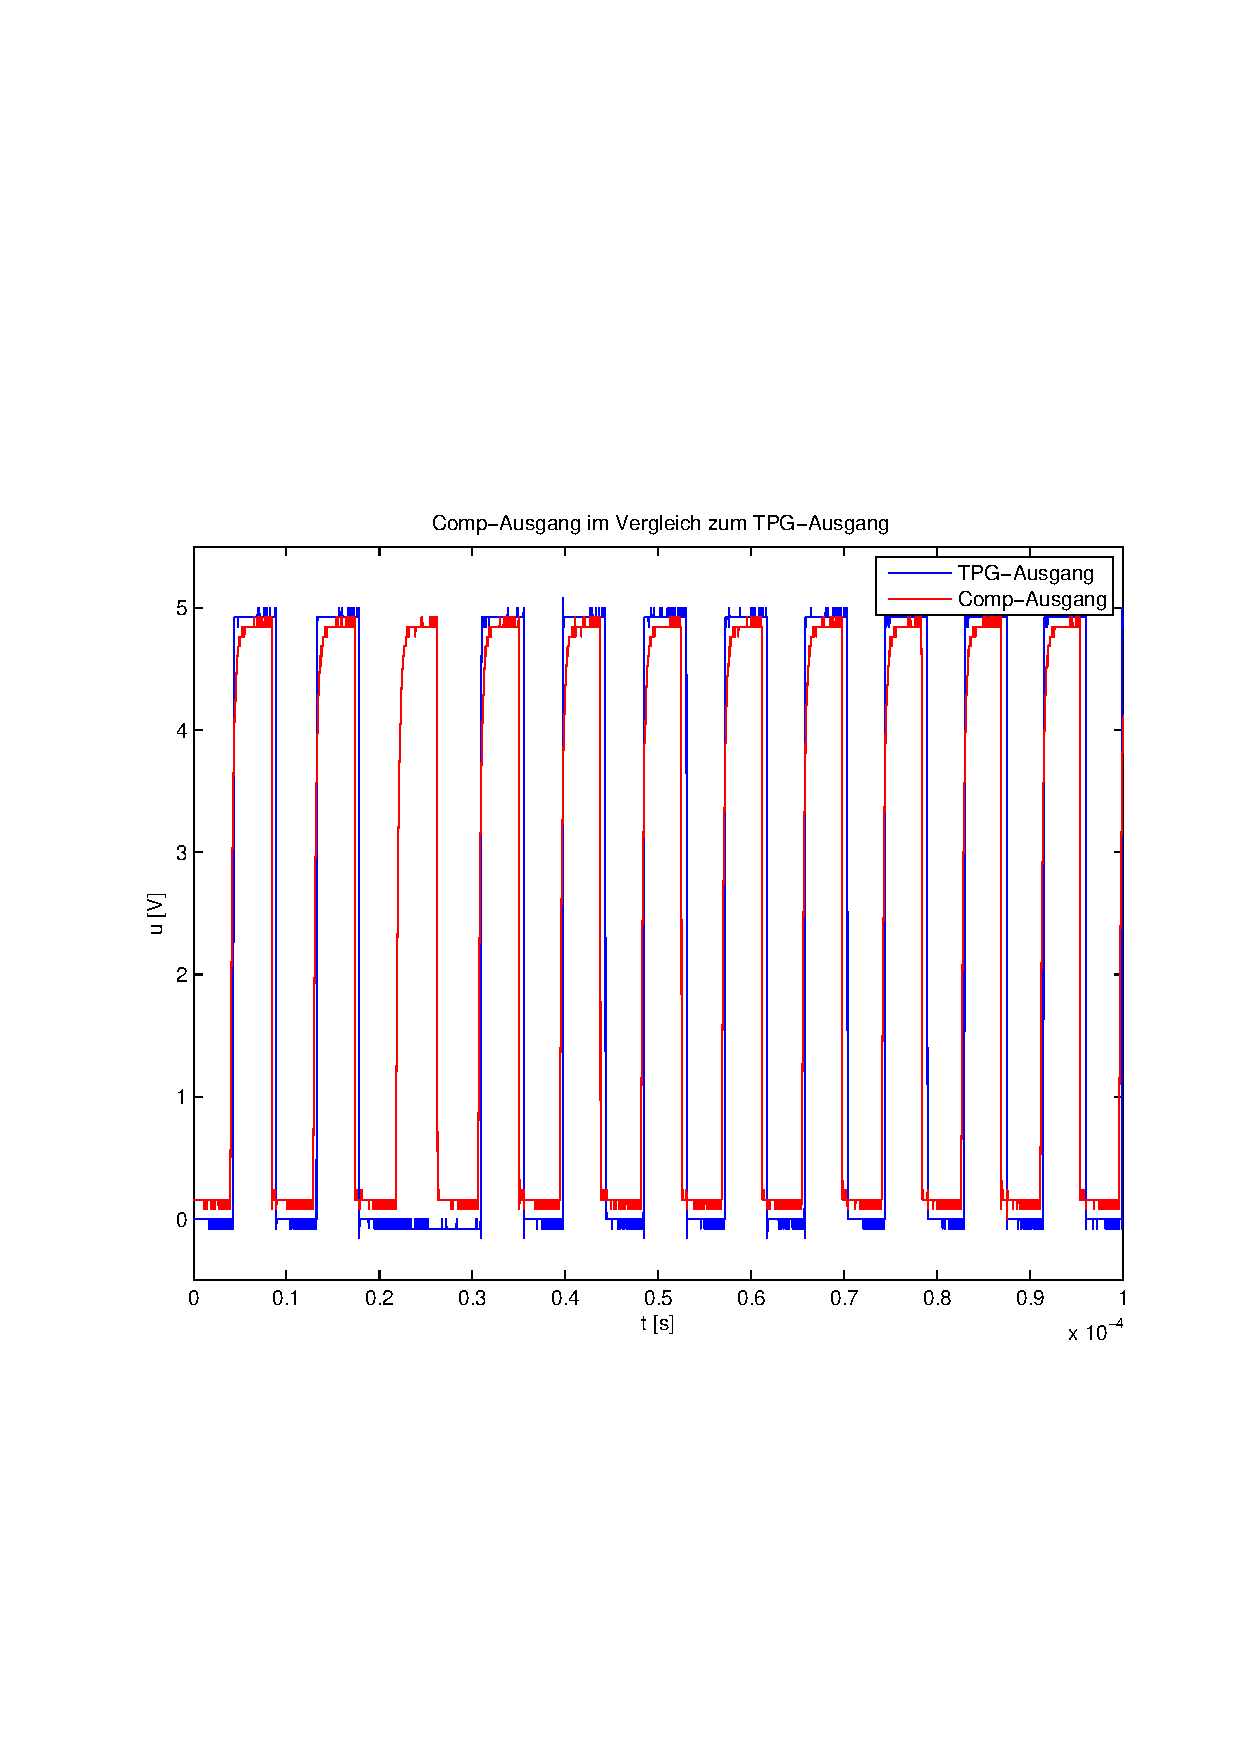
\includegraphics[scale=0.5, trim = 2cm 6.5cm 1.5cm 8.5cm,
                    clip]{./Bilder/comp_vs_tpg}
                        \caption{Vergleich zwischen Comparator- und
                        TPG-Ausgangssignal}
                \end{figure}
          
          Man kann deutlich sehen, dass beide Ausgänge einen sehr ähnlichen
          Verlauf haben, der TPG aber manchmal nicht mit dem Comp-Ausgang
          mitkommt und eine steigende Flanke überspringen kann, wodurch eine
          Störung in der Rechteckperiode entstehen kann.\\
          
          Zuletzt wurde das Sendesignal mit fester Frequenz in den Vergleich mit
          dem moduliert-demoduliertem Signal gesetzt. Das folgende Ergebnis kam
          heraus:
          
           
             \begin{figure}[H] \centering
                    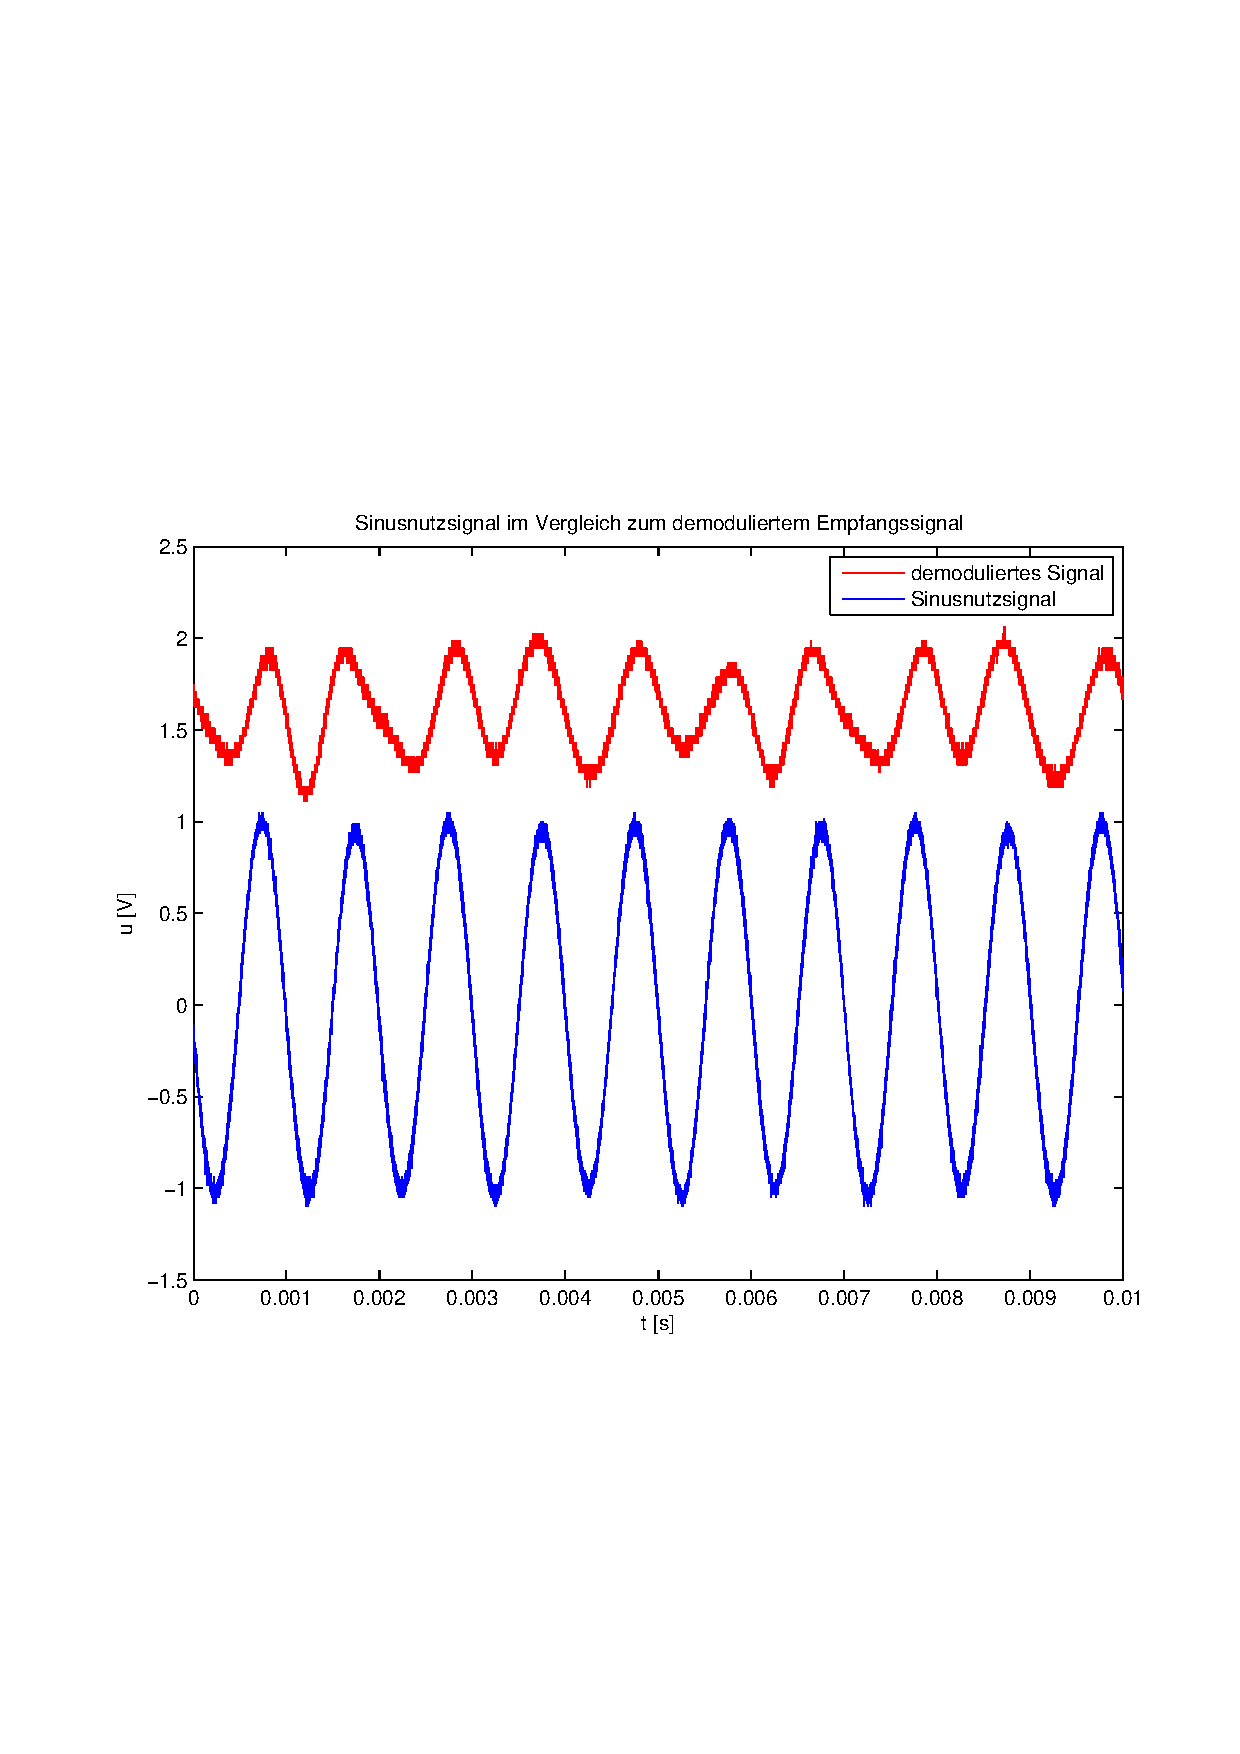
\includegraphics[scale=0.5, trim = 2cm 6.5cm 1.5cm 8.5cm,
                    clip]{./Bilder/sinus_fm_demod}
                        \caption{Vergleich zwischen festem Sendesignal und
                        demoduliertem Empfangssignal}
                \end{figure}
          
        Das demodulierte Signal besitzt einen Offset und keine sehr klaren
        Sinusverlauf. Daraus lässt sich schließen, dass die FM-PFM-Umwandlung
        für eine FM-Demodulation eines Sinussignals nicht sehr geeignet ist.\\
        (müssen wir hier mehr dazu schreiben??)
    \end{quote}	
\end{quote}

%--------------------------------------------------------------------
%--------------------------------------------------------------------    

\section{Zusammenfassung}
\begin{quote}
	
\end{quote}

%--------------------------------------------------------------------
%--------------------------------------------------------------------    


\begin{thebibliography}{999}
\bibitem {AMohnetraeger} Prof. Dr.-Ing. Sikora, Thomas; Prof. Dr.-Ing. Noll, Peter: Einführung in die
Nachrichtenübertragung, S.207
\bibitem {AMdemodulation} Prof. Dr.-Ing. Sikora, Thomas; Prof. Dr.-Ing. Noll, Peter: Einführung in die
Nachrichtenübertragung, S.209
\bibitem {AMohneUeber} Prof. Dr.-Ing. Sikora, Thomas; Prof. Dr.-Ing. Noll, Peter: Einführung in die
Nachrichtenübertragung, S.206
\bibitem {AMmitUeber} Prof. Dr.-Ing. Sikora, Thomas; Prof. Dr.-Ing. Noll, Peter: Einführung in die
Nachrichtenübertragung, S.215



%Name, Vorname.; evtl. Name2, Vorname2.: Titel des Dokumentes
%oder Buches, Zeitschrift/Verlag/URL (Auflage, Erscheinungsort, -jahr), ggf. Seitenzahlen
% \bibitem {PasevalscheTheorem} \url{https://de.wikipedia.org/wiki/Parsevalsches_Theorem}, Zugriff
% 23.05.2012
\end{thebibliography}

\end{document}
